\documentclass[10pt,a4paper]{book}
%----------------------------------------------------------
% This is a sample document for the standard LaTeX Book Class
% Class options
%       --  Body text point size:
%                        10pt (default), 11pt, 12pt
%       --  Paper size:  letterpaper (8.5x11 inch, default)
%                        a4paper, a5paper, b5paper,
%                        legalpaper, executivepaper
%       --  Orientation (portrait is the default):
%                        landscape
%       --  Printside:   oneside, twoside (default)
%       --  Quality:     final(default), draft
%       --  Title page:  titlepage, notitlepage
%       --  Columns:     onecolumn (default), twocolumn
%       --  Start chapter on left:
%                        openright(no, default), openany
%       --  Equation numbering (equation numbers on right is the default):
%                        leqno
%       --  Displayed equations (centered is the default):
%                        fleqn (flush left)
%       --  Open bibliography style (closed bibliography is the default):
%                        openbib
% For instance the command
%          \documentclass[a4paper,12pt,reqno]{book}
% ensures that the paper size is a4, fonts are typeset at the size 12p
% and the equation numbers are on the right side.


\usepackage[left=2.5cm, right=2cm, top=2cm, bottom=2cm]{geometry}
\usepackage[latin1]{inputenc}
\usepackage[T1]{fontenc}
\usepackage{pdflscape}
\usepackage[colorlinks,pdfpagelabels,pdfstartview = FitH,bookmarksopen = true,bookmarksnumbered = true,linkcolor = black,plainpages = false,hypertexnames = false,citecolor = black] {hyperref}

\usepackage{amsmath}
\usepackage{amsfonts}
\usepackage{amssymb}
\usepackage{amsthm}
\usepackage{upgreek}


\usepackage{graphicx}
\usepackage{color}
\usepackage{tikz}
	\usetikzlibrary{shapes,arrows}
\usepackage{dirtree}

\usepackage{tabularx}
%\usepackage{ltablex}
\usepackage{multicol}

\usepackage{listings}
\usepackage{blindtext}

\usepackage{float}
\usepackage[section]{placeins}
\usepackage{wrapfig}
\usepackage{caption}
\usepackage{subcaption}


%\usepackage[printonlyused,withpage]{acronym}
\usepackage{makeidx}
\usepackage{cite}
\usepackage[acronym,shortcuts,toc]{glossaries}

%%%%%%%%%%% Personal commands %%%%%%%%%%%%%%%%%

\newcommand{\software}{{\scshape TOM }}
\newcommand{\matlab}{{\scshape MATLAB }}
\newcommand{\omen}{{\scshape OMEN }}

\theoremstyle{remark}
\newtheorem*{REMARK}{Remark}
\newtheorem*{EXAMPLE}{Example}

%%%%%%%%%%%%%%%%%%%%%%%%%%%%%%%%%%%%%%%%%%%%%%%


\lstset{language=Matlab}
\setlength\parindent{0pt}

\makeindex
\makeglossaries

\definecolor{mygreen}{rgb}{0,0.6,0}
\definecolor{mygray}{rgb}{0.5,0.5,0.5}
\definecolor{mymauve}{rgb}{0.58,0,0.82}

\lstset{ %
  backgroundcolor=\color{white},   % choose the background color; you must add \usepackage{color} or \usepackage{xcolor}
%  basicstyle=\footnotesize,        % the size of the fonts that are used for the code
  breakatwhitespace=false,         % sets if automatic breaks should only happen at whitespace
  breaklines=true,                 % sets automatic line breaking
  captionpos=b,                    % sets the caption-position to bottom
  commentstyle=\color{mygreen},    % comment style
  deletekeywords={...},            % if you want to delete keywords from the given language
  escapeinside={\%*}{*)},          % if you want to add LaTeX within your code
  extendedchars=true,              % lets you use non-ASCII characters; for 8-bits encodings only, does not work with UTF-8
  frame=single,                    % adds a frame around the code
  keepspaces=true,                 % keeps spaces in text, useful for keeping indentation of code (possibly needs columns=flexible)
  keywordstyle=\color{blue},       % keyword style
  language=Matlab,                 % the language of the code
  morekeywords={*,...},            % if you want to add more keywords to the set
  numbers=left,                    % where to put the line-numbers; possible values are (none, left, right)
  numbersep=5pt,                   % how far the line-numbers are from the code
  numberstyle=\tiny\color{mygray}, % the style that is used for the line-numbers
  rulecolor=\color{black},         % if not set, the frame-color may be changed on line-breaks within not-black text (e.g. comments (green here))
  showspaces=false,                % show spaces everywhere adding particular underscores; it overrides 'showstringspaces'
  showstringspaces=false,          % underline spaces within strings only
  showtabs=false,                  % show tabs within strings adding particular underscores
  stepnumber=2,                    % the step between two line-numbers. If it's 1, each line will be numbered
  stringstyle=\color{mymauve},     % string literal style
  tabsize=2,                       % sets default tabsize to 2 spaces
  title=\lstname                   % show the filename of files included with \lstinputlisting; also try caption instead of title
}

%\includeonly{Chapters/SolarCell, Chapters/Analysis, Chapters/matlab}

\newacronym{GUI}{GUI}{Graphical User Interface}
\newacronym{CQD}{CQD}{Colloidal Quantum Dot}

\begin{document}
	\frontmatter
	\newcommand{\trtitle}{Simulation of Quantum Dots}
\newcommand{\trtype}{Group project}
\newcommand{\trprofone}{Prof. Vanessa Wood}
\newcommand{\trproftwo}{Prof. Mathieu Luisier}
\newcommand{\trresearchgroup}{Laboratory for Nanoelectronics}
\newcommand{\trinstitute}{Integrated Systems Laboratory}
\newcommand{\trdepartment}{Department of Information Technology \& Electrical Engineering}
\newcommand{\truni}{ETH Zurich}
\newcommand{\trdate}{\today}

\thispagestyle{empty}


\includegraphics[scale=0.8]{Fig/eth_logo_black.pdf}

\rule{\textwidth}{0.4pt}

\vspace{2.5cm}
\begin{center}
  \textbf{\LARGE \trtitle}
\end{center}
\vspace{2cm}

\begin{center}
  \textbf{\trtype}	\\
  \trresearchgroup	\\
  \trprofone				\\
  \trinstitute			\\
  \trdepartment			\\
  \truni						\\[0.5cm]
  Handed in by			\\
  \textbf{Christian Funck \& Matthias Dittberner}	\\[0.5cm]
  Date							\\
  \trdate						\\
\end{center}

\vspace{1cm}

\begin{center}
	\begin{tabular}{ll}
		Supervisor: & \trprofone	\\
								& \trproftwo	\\
	\end{tabular}
\end{center}

\vfill

%\begin{tabularx}{\textwidth}{lr}
\begin{tabular*}{\textwidth}{@{\extracolsep{\fill} } lr}
%\begin{tabular}{@{}p{0.5\textwidth}>{\raggedright\arraybackslash}{p{0.5\textwidth}}}
	Christian Funck					&	Matthias Dittberner				\\
	Plattenstrasse 71				&	Luegislandstrasse 269			\\
	8032 Zurich							&	8051 Zurich								\\
	09-920-177							& 09-913-450								\\
	cfunck@student.ethz.ch	&	mdittber@student.ethz.ch	\\
\end{tabular*}

\rule{\textwidth}{0.4pt}
	
	\cleardoublepage\pdfbookmark{\contentsname}{toc}		% Add Table of Contents to the PDF bookmarks
	\tableofcontents
	\newpage


	\mainmatter

	\chapter{The Quantum Dot} \label{sec:QuantumDot} \index{Quantum Dot}

	Quantum dots are atomic structures (usually spherical) that have a size of about 1-10nm in diameter. They are often referred to as \glspl{NC}, though this
	term is more general and includes also other shapes and morphologies, which might extend to several $\mu$m, such as rods, wires etc.
	Figure \ref{fig:QDshapes} gives some examples of possible shapes and morphologies, that are possible with nowadays technologies.
	
	\glspl{QD} are possible with various materials such as metals, semiconductors and compounds. According to their size and material,
	a \glspl{QD} can contain just a few or millions of atoms. A 10nm cube of GaAs contains for example 40,000 atoms \cite{SalehTeich}.
	
	The properties of \glspl{QD} are strongly dependent on their size. Figure \ref{fig:QDTheory} illustrates this effect for a semiconductor \gls{QD}.
	Under ultraviolet excitation, the \glspl{QD} emit light according to their size and therefore band gap.
	
	\begin{figure}[htbp]
		\begin{minipage}[t]{0.49\textwidth}
			\centering
			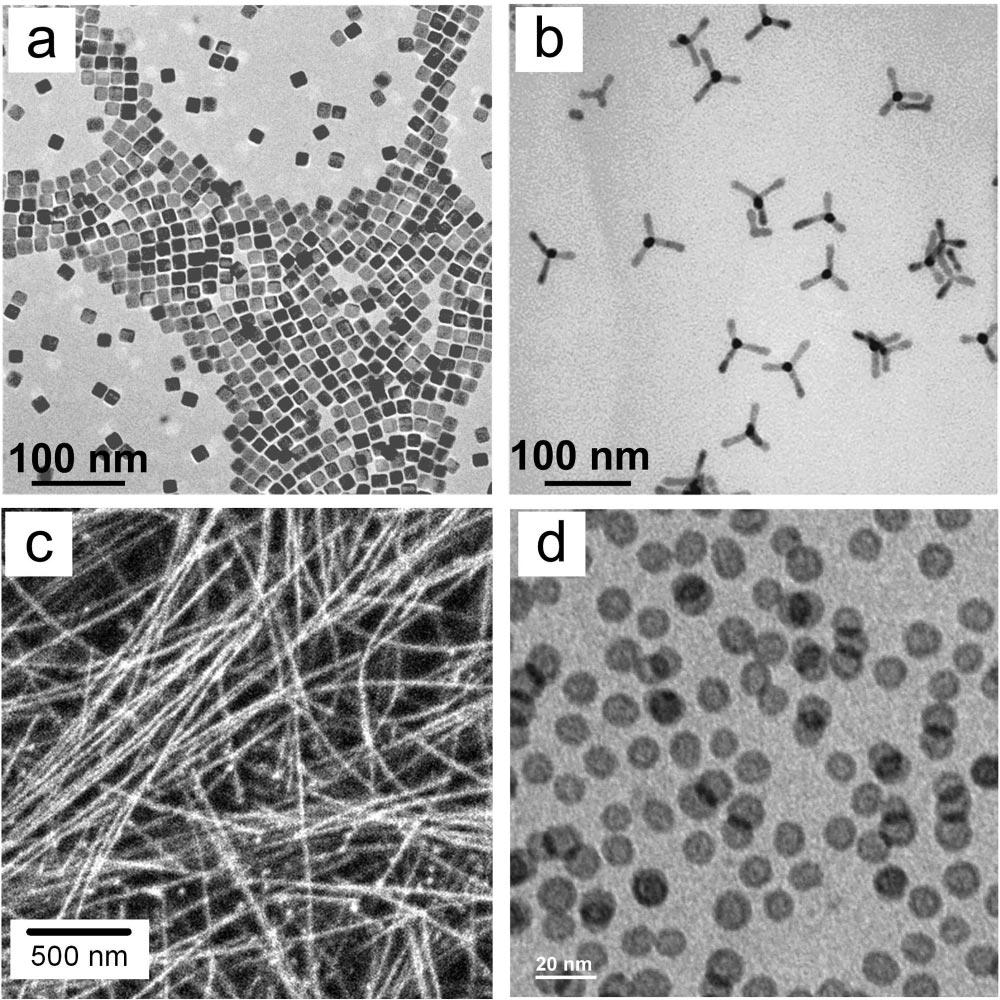
\includegraphics[width=\textwidth]{Fig/QDshapes.jpg}
			\caption{Examples of inorganic nanomaterials with different
							 shapes and morphologies synthesized by colloidal chemistry:
							 (a) PbSe cubes; (b) CdTe tetrapods; (c) PbSe nanowires and
							 (d) hollow iron oxide nanoparticles.
							 {\scshape Source:} \cite[p.394]{Talapin}}
			\label{fig:QDshapes}
		\end{minipage}
		\hfill
		\begin{minipage}[t]{0.49\textwidth}
			\centering
			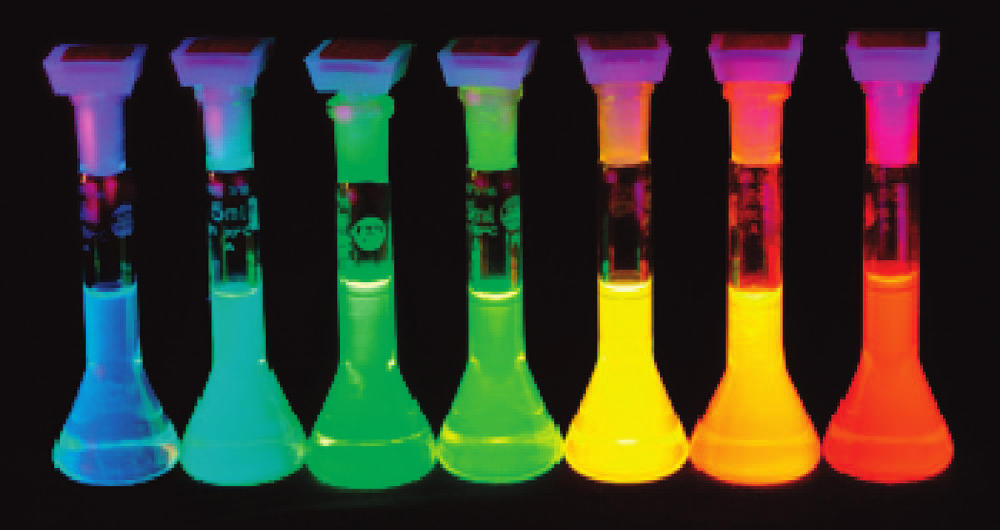
\includegraphics[width=\textwidth]{Fig/QDcolor.jpg}
			\caption{This photograph shows the size-dependent \gls{PL} of the quantum dots. The particles with the smallest ($\sim$1.7nm)
							 CdSe cores emit blue and those with the largest cores ($\sim$5nm) emit red.
							 {\scshape Source:} \cite[p.393]{Talapin}}
			\label{fig:QDcolor}
		\end{minipage}
	\end{figure}			

	\paragraph{Basic physics of the Quantum Dot}
		For bulk materials the band gap \index{Band gap} is a fixed parameter, that specifies the type of material. But when a particle gets smaller and reaches
		a size of about 10nm this will not be the case anymore. The band gap is than depending on the size of this particle (\glspl{NC}). As
		the mobility of the charge carriers (electrons, holes) is very limited in all three dimensions in the quantum dot, the energy levels
		are not continuous, but instead discrete.
		This phenomenon is called the {\it quantum size effect}.
		
		The band gap \index{Band gap} of a spherical \gls{QD} of radius $R$ is then approximately:
		\begin{equation}
			E_{g} \approx E_{g,0} + \frac{\hbar^2 \pi^2}{2 m_{eh} R^2}
			\label{eq:Bandgap}
		\end{equation}
		where $E_{g,0}$ denotes the band gap of the bulk material and $m_{eh}$ is obtained through the effective masses of electrons and holes $m_{e,p}$:
		\begin{equation}
			m_{eh} = \frac{m_e m_h}{m_e + m_h}
			\label{eq:QuantumBox}
		\end{equation}
		
		\begin{figure}[htbp]
			\centering
			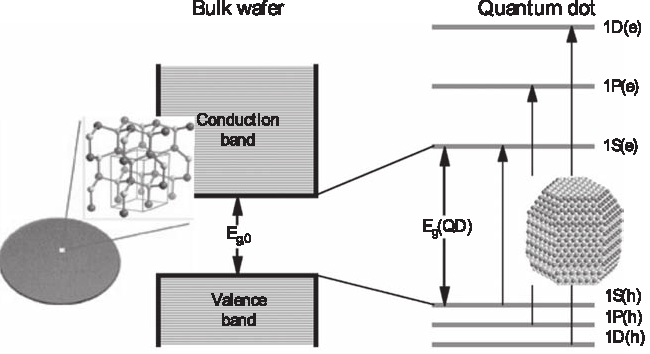
\includegraphics[width=0.4\textwidth]{Fig/QDTheory.pdf}
			\caption{The left illustration shows the band structure of a bulk semiconductor with energy band gap $E_{g,0}$,
							 whereas the the right one illustrates the discrete energy levels of a \gls{QD} and its energy gap $E_{g}(QD)$.
							 {\scshape Source:} \cite[p.3]{Klimov}}
			\label{fig:QDTheory}
		\end{figure}
		
		
		We will see later in chapter \ref{sec:BandGapAnalysis} that the \gls{QD} absorption spectrum \index{Absorption spectrum} as shown in figure \ref{fig:QDTheory}(c) is not really discrete; as it is
		not possible to fabricate \glspl{QD} that are perfectly equal in size, this results in a broadening of the spectrum.
		The energy gap increases for decreasing \gls{QD} sizes, because more energy is required to confine the electron to a smaller volume.
		This is caused by Heisenberg's uncertainty principle \index{Heisenberg uncertainty principle}, which says, that if we want to locate a particle of effective mass $m$ (for example an electron),
		on an x-axis within an interval	$\Delta x$, we can only make an uncertain prediction of its impulse. If the spatial region gets smaller, the uncertainty
		of the impulse will	increase.
		\begin{equation}
			\Delta p_{x} \sim \frac{\hbar}{\Delta x}
		\end{equation}
		This adds to the kinetic energy of the free particle, which is called the confinement \index{Confinement} energy \index{Confinement!Energy}, that has an significant impact, if it gets bigger
		than the thermal energy of the particle.
		\begin{equation}
			E_{confinement} = \frac{(\Delta p_{x})^2}{2 m} \sim \frac{\hbar^2}{2 m (\Delta x)^2} > \frac{1}{2} k_{B} T
		\end{equation}
		From this we can conclude, that the quantum size effect is relevant if
		\begin{equation}
			\Delta x < \sqrt{\frac{\hbar^2}{m k_{B} T}}
		\end{equation}
		Table \ref{tbl:ConfinedStr} shows 4 possible confinement structures\index{Confinement!Structure}, which are illustrated in Figure \ref{fig:ConfinedStr} with their
		characteristic energy levels \index{Energy level} in	the conduction band.

		\begin{figure}[htbp]		
		\centering
		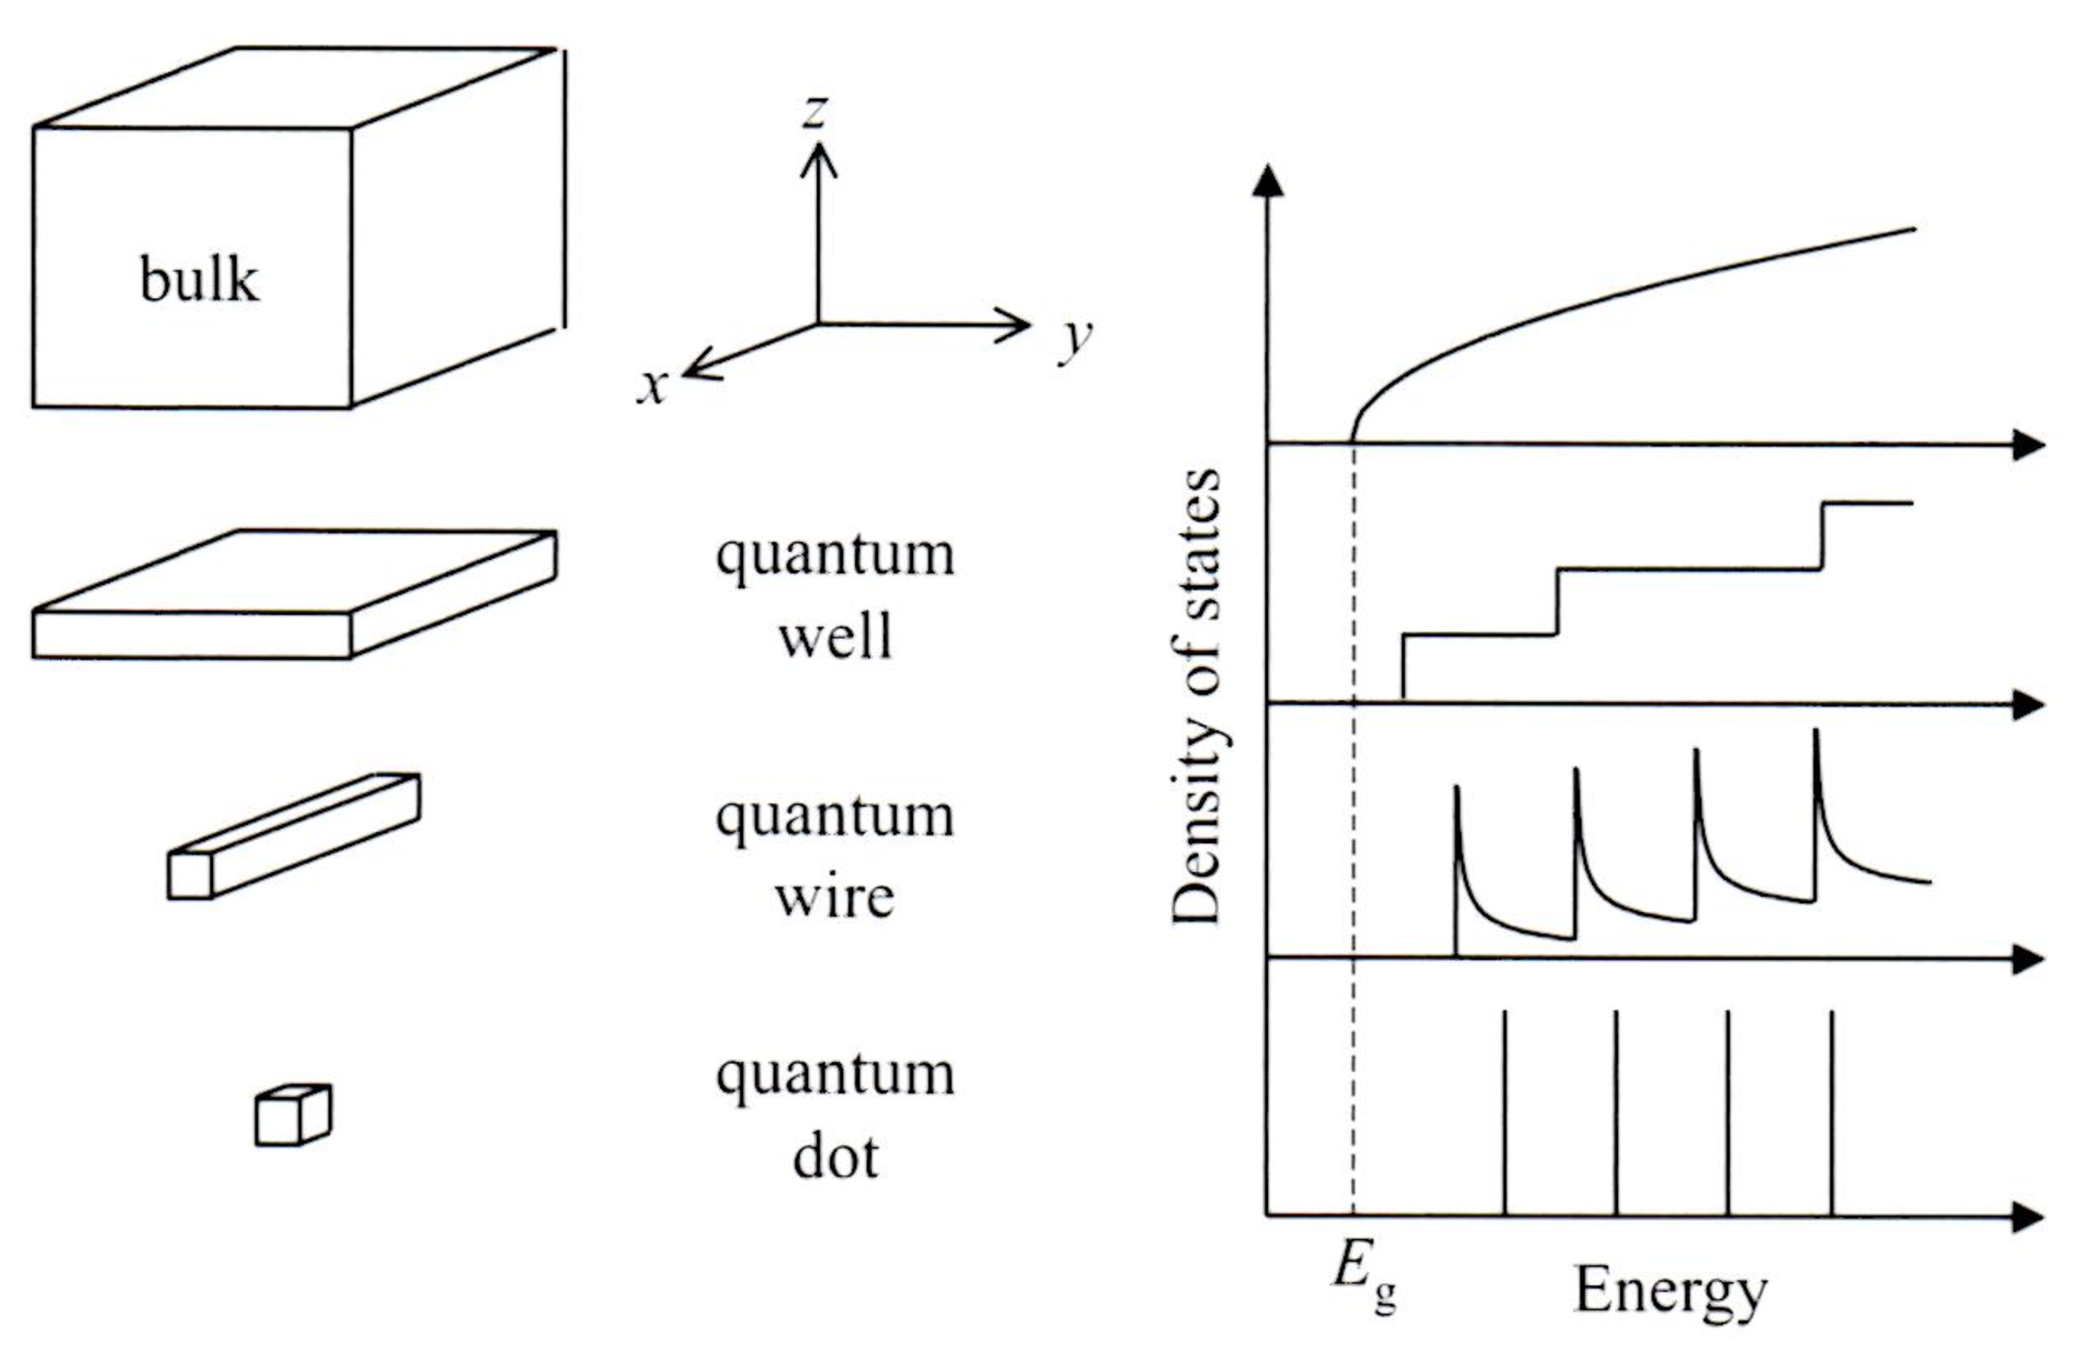
\includegraphics[width=0.5\textwidth]{Fig/ConfinedStructures.pdf}
		\caption{Schematic representation of quantum wells, wires and dots (left).
						 The generic shape of the density of states function for electrons in the
						 conduction band of a semiconductor with band gap $E_{g}$ is shown for each
						 type of the structure (right).
						 {\scshape Source:} \cite[p.143]{Fox}}
		\label{fig:ConfinedStr}
	\end{figure}
		
		\begin{table}[htbp]
		\centering
			\begin{tabular}{lccc}
				Structure											&	Quantum				&	\# of free		&	Electron						\\
																			&	confinement		&	dimensions		&	density of states		\\
				\hline
				Bulk													&	none					&	3							&	$\propto E^{1/2}$		\\
				Quantum well/superlattice			&	1-D						&	2							&	$\propto E^{0}$			\\
				Quantum wire									&	2-D						&	1							&	$\propto E^{-1/2}$	\\
				Quantum dot/box								&	3-D						&	0							&	discrete						\\
			\end{tabular}
			\caption{Number of degrees of freedom tabulated against the dimensionality of the quantum confinement.
							 The final column shows the functional form of the density of states for free electrons.
							 {\scshape Source:} \cite[p.142]{Fox}}
			\label{tbl:ConfinedStr}
		\end{table}
	
	\paragraph{Fabrication techniques of \gls{QD}}
	
		A lot of different ways to make \glspl{QD} have been developed. Research efforts are made to create
		more efficient \glspl{QD} and new shapes and morphologies. As \glspl{QD} are more and more interesting for various commercial applications,
		low costs play an important factor. The colloidal chemistry has made a major contribution, as it offers low energy
		synthesis of \glspl{NC}/\glspl{QD} using very simple and affordable laboratory equipment.		
		In the next chapter we will briefly discuss the mentioned technique, by giving a short overview
		that avoids the use of chemical terms as much as possible, rather than a detailed disquisition, as this is a research field on its own.
		
		Some other methods are listed below.
	
		\begin{tabularx}{\textwidth}{Xl}
			{\bf Physical methods}														&	{\bf Characterization}										\\
			Molecular-beam-epitaxy (MBE)											& High-energy-input, expensive apparatus,
																													used	for \glspl{QD}											\\
			Metalorganic-chemical-vapor-decomposition (MOCVD)	&	High-energy-input, used for \glspl{QD}		\\
			Vapor-liquid-solid (VLS)													&	High-energy-input, used for quantum wires	\\
			Electron-beam lithography													&			\\
																												&			\\
			{\bf Chemical methods}														&	{\bf Characterization}										\\
			Colloidal chemical synthesis of crystalline
			semiconductor nanoparticles												& Low-energy-input, wet chemistry,
																													used for various structures								\\
		\end{tabularx}
	
		
		
	\paragraph{Applications}
		
		In biology and chemistry \glspl{QD} are used as spectral tags that are attached to molecules, making their position visible for identification
		under optical illumination. In the past, one used organic dyes, but compared to \glspl{QD} the sharpness of emission lines is not as good.
		
		In electronics, \glspl{QD} are used to increase the efficiency of lasers \cite{SemiconductorCD}, everyday light sources and solar cells.
		Furthermore they are used	in broadband \gls{LED}, memory elements, flexible displays, photodetectors.
		
		We have to add that a lot of these applications are still developed in research institutions and are not yet available for commercial use.
		
		Although the applications seem impressive and will probably motivate new technologies, there are reasonable concerns about these nanoscale
		particles. Some of the materials are toxic and through the small sizes it is unclear what might happen if the particles end up in living
		organisms or generally speaking, into the the environment.
		For more interested readers, we recommend the following paper for further reading: \citeauthor{Hardman} \citetitle{Hardman} \cite{Hardman}.
	\chapter{QD Solar Cells}

This chapter gives a brief overview over the fundamental principles of photovoltaic cells and QD solar cells in particular, then focusing on the example of PbS cells to give some specific information.

\section{Solar Cell Principles}

% FIGURE
\begin{figure}
	\centering
	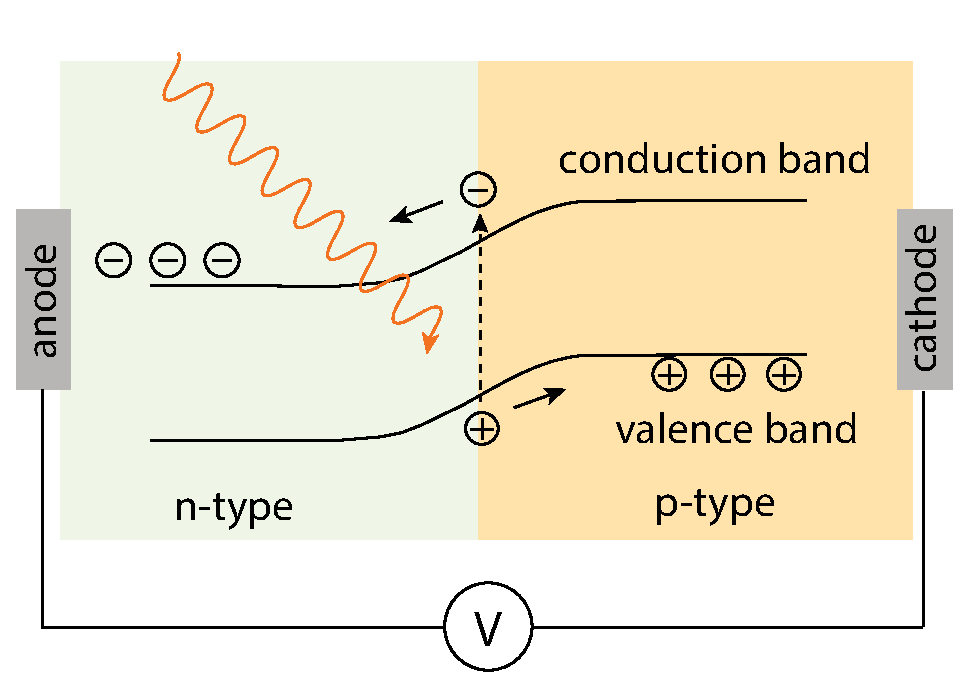
\includegraphics[width=200px]{Fig/SolarCell/pnSolarCell}
	\caption{Principle of a solar cell using a p-n semiconductor junction.}
	\label{fig:pnSolarCell}
\end{figure}

\begin{figure}
	\centering
	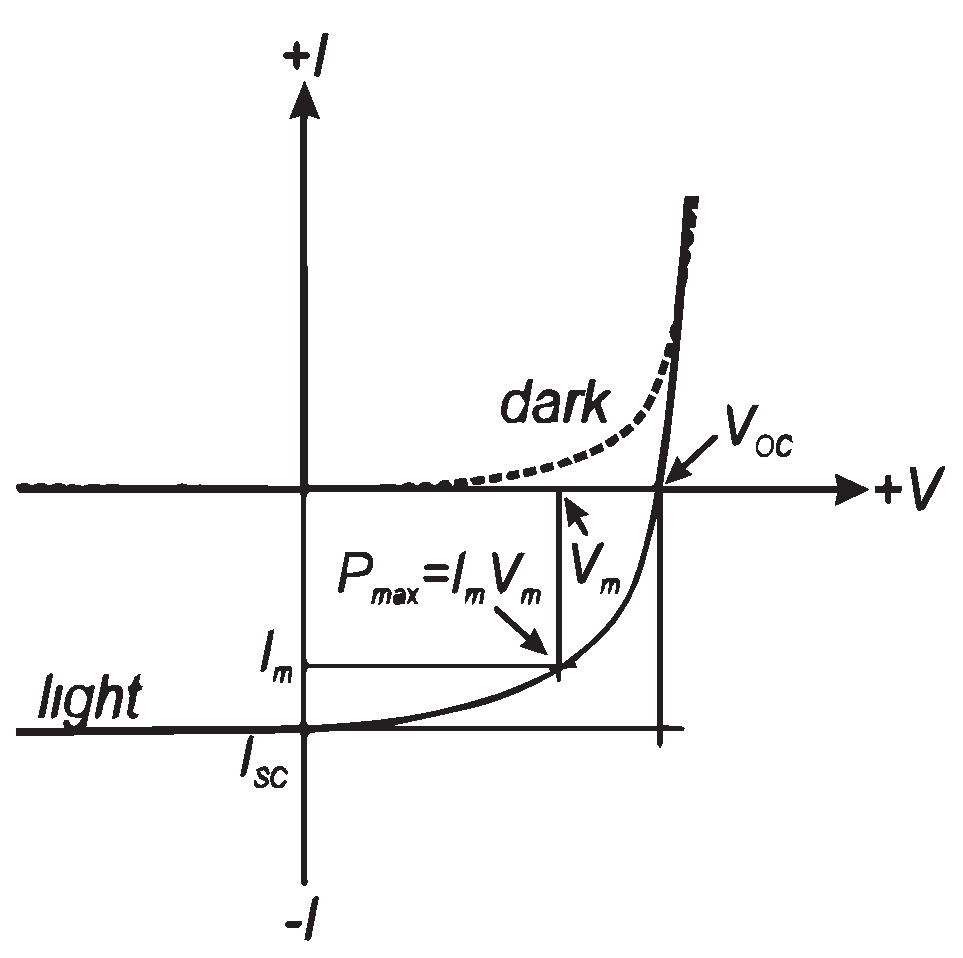
\includegraphics[width=200px]{Fig/SolarCell/IVsolarCell}
	\caption{Typical I-V characteristics of a solar cell. \scshape{Source:} \cite[p.427]{Talapin}}
	\label{fig:IVsolarCell}
\end{figure}

% TEXT
The basic idea of a solar cell is to convert light into electrical power. Light is absorbed in a material, thus generating an electron-hole pair. The generated electrons and holes must then be separted and conducted to electrodes attached to the material. The accumulation of carriers at the electrodes generates a potential difference, and a current will flow between the electrodes, if a load is connected.

The carrier separation can be achieved by an electirc field inside the material. Different types of solar cells exist based on different approaches. The typical silicon solar cell uses a semiconductor p-n junction: When a photon (with energy greater than the band gap) is absorbed in the semiconductor, an electron is promoted from the valence to the conduction band. Near the junction, these photogenerated electrons and holes are swept away to different sides, due to the built-in electric field of the p-n junction (fig.~\ref{fig:pnSolarCell}). 

Other approaches are also widely used, for example Schottky contacts (metal-semiconductor interface) or semiconductor-liquid interfaces.\\

The electrical behaviour of a photovoltaic cell can be well described by its I-V characteristics (fig.~\ref{fig:IVsolarCell}). In the dark, the cell behaves like a diode (in the case of a p-n junction solar cell this seems fairly obvious). Under illumination, the curve is shifted vertically downwards. It crosses now the fourth quadrant, where the electrical power $P=IV$ is negative, which indicates that power is delivered to the load.\\

To characterise the solar cell, there are some common parameters, which are mentioned in the following paragraph. The open-circuit voltage $V_{OC}$ is the maximum voltage provided by the cell. It is directly related to the energy band structure and thus to the built-in potential. The short-circuit current $I_{SC}$ gives the maximum current, which flows if the electrodes are connected. $I_{SC}$ is proportional to the carrier density under illumination and to the carrier mobility, which are therefore important parameters to maximize.

An often used quantity is the \textit{fill factor (FF)}, which is the ratio between the maximum power $P_M=I_M V_M$ and the product $I_{SC} V_{OC}$. It describes how well behaved the I-V characteristics is (the more the curve approaches a rechtangular shape, the better).

Of practical importance for comparing solar cells is the power conversion efficiency $\eta$, giving the ratio of optical power which is converted into electrical power. 
\[\eta = \frac{P_{max}}{P_{in}} = FF\frac{I_{SC}V_{OC}}{P_{in}}\]
Usually an optical source called AM1.5 is used, whose spectral intensity distribution matches that of sunlight reaching the earth's surface at an angle of $48.2^{\circ}$. \cite[pp.426-433]{Talapin}

\section{Solar Cells using QDs}

Semiconductor nanocrystal solids, can be used for solar cells. Thus nanocrystals (NC) made of CdSe, CdTe, PbSe, PbS and many more can be used for this purpose. Like with bulk semiconductors, heterojunction solar cells are possible (using materials with different band gaps), such as CdSe-CdTe cells \cite[p.430]{Talapin}. Similarly, using Schottky-contacs is also an option.\\

Using NC solids made of QDs offers several advantages. One big advantage is the possibilty of choosing the size of the band gap by controlling the size of the QDs, which can be done easily during the synthesis of CQDs. Controlling the band gap means essentially choosing the spectrum which can be absorbed, and consequently cells, which can make use of a broad spectrum, can be engineered.

Furthermore QD solar cells are easy to fabricate and that at low costs. Large-scale production would also be possible \cite[p.447]{Talapin}.

Using NC solids, there are promising perspectives for more advanced techniques, in order to increase efficiency. These invlove e.g.~carrier multiplication (the absorption of one highly energetic photon causes the creation of multiple electron-hole pairs) or hot carrier solar cells (electrons in higher energy states in the conduction band are extracted before they relax to the band edge and lose some energy).\\

However, there are some problems which have to be overcome. One is the (air-) stability and lifespan of QD based photovoltaic cells. In many cases, the devices lose dramatically in efficiency after some time, which can be as short as hours or even minutes \cite[p.26]{Tang2011}. Another problem is the currently rather low efficiency of the cells (maxium acchieved efficiency of around 7\% for a PbS cell \cite[p.1]{Ip2012}). One issue leading to reduced efficiency is the presence of undesired states in the band gap (mid-gap or trap states). These arise due to `dangling' (unbound) bonds of surface atoms, and are significant in a QD, since its surface to volume ratio is high. So-called \textit{passivation} of the surface is thus very important. 

Furthermore, for furture large-scale production, the materials used in the production process should be cheap,  available in large quantities and preferably non-toxic, which contrasts with some NC materials that contain toxic elements like Cd or Pb.

\subsection{Example of a PbS QD Solar Cell}

% FIGURES

\begin{figure}
	\centering
	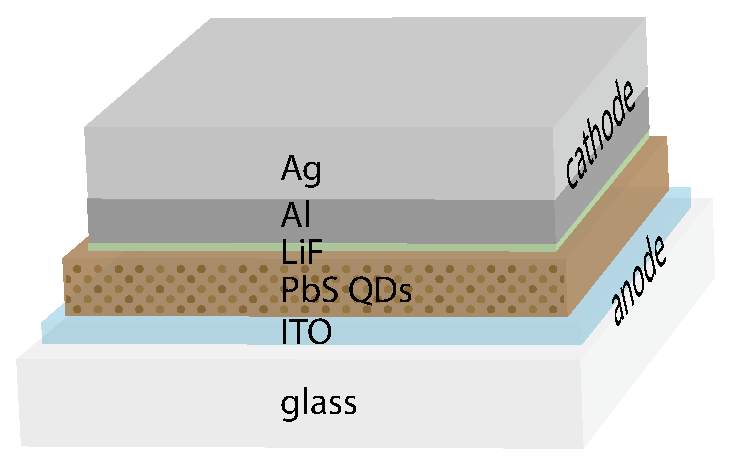
\includegraphics[width=200px]{Fig/SolarCell/PbSsolarCellStructure}
	\caption{Structure of a PbS solar cell.}
	\label{fig:PbSsolarCellStructure}
\end{figure}

% TEXT

Since the structure and fabrication methods of QD solar cell are quite diverse, we will focus here on a PbS QD solar cell, as they were produced at ETH at the Laboratory for Nanoelectronics \cite{MS_Michael}. Due to the small band gap of PbS (0.37eV for bulk PbS), the solar cell is able to convert power from the near infrared spectrum. This is of interest, since roughly 50\% of the solar energy that reaches the earth is in the infrared spectrum.

\subsubsection{Structure}

The principle part of the cell is a Schottky junction of PbS and Al, with a thin protection layer (1 nm) of LiF in between. The Schottky barrier is responsible for the electric field which separates the photogenerated carriers. The Al Cathode is covered by a layer of silver, for better air stability. The transparent anode is formed of a layer of indium tin oxide (ITO), on top of the PbS (fig.~\ref{fig:PbSsolarCellStructure}).

\subsubsection{Fabrication Process}

The main steps involved in the fabrication are described below, as they were carried out in reference \cite[pp. 13-19]{MS_Michael}.

We start with a glass substrate, which is coated with ITO using lithography. The sample has then to be cleaned (using solvents, and afterwards by $O_2$ plasma treatment to remove organic residuals). 

In the next step, the active layer, i.e.~the PbS QDs, is deposited. This can be done by dip coating, where the substrate is immersed in a PbS-hexane solution, and taken out after a few seconds, leaving a thin film of the solution on the sample. Alternatively, spin coating can be used, where several drops of the PbS-Hexane solution are dropped on the substrate, which is then rotated to spread the drops, leading to a film of homogeneous thickness. 

Now the long ligands surrounding the QDs have to be exchanged for short ligands, in order to improve inter-particle coupling (and thus e.g.~carrier mobility). For this purpose, the substrate is immersed into a suitable compound: Ethandithiol, benzenedithiol (both organic), and ammonium thiocyanate ($NH_4SCN$, inorganic) can be used.

The sample is then rinsed in acetonitrile and or hexane. In order to obtain a PbS film of desired thickness, the steps of spin (respectively dip) coating, ligand exchange and rinsing have to be repeated several times.

In a last step, the cathode, i.e.~the three layers of LiF, Al and Ag are evaporated on the substrate.
	
	\chapter{Analysis of PbS QD simulation data}

In this chapter we will take a look at the simulation data, which are based on a tight-binding model used by \omen. The parameters used for the simulation can be found in appendix \ref{sec:SimPar} on page \pageref{sec:SimPar}. We will make an analysis of the energy levels and wave functions of PbS QDs and draw some conclusions.\\

\begin{REMARK} 
There are a few practical aspects to note concerning the simulation of PbS QDs with OMEN: Since \omen will consider in its calculation 18 orbitals for the atoms, one must keep in mind that the simulation uses significantly more computing resources than a simulation of a CdSe-CdS QD for instance. Especially the memory usage during the calculation can easily exceed 10GB for larger QDs. The size of the generated simulation data for one QD can also amount to more than a few 100MB. It has to be kept in mind, that the number of atoms scales with the third potence of the radius. Another problem is the high degeneracy of energy levels. This makes it necessary to simulate a higher number of modes, thus increasing the usage of resources further.
\end{REMARK}

\section{Energy levels}
%ENERGY LEVELS

%FIGURES
\begin{figure}
	\centering
	\begin{subfigure}{60px}
		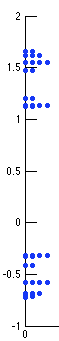
\includegraphics[height=150px]{Fig/Plots/r1b.png}
		\caption{}
	\end{subfigure}    
	\begin{subfigure}{60px}
		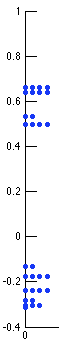
\includegraphics[height=150px]{Fig/Plots/r3b.png}
		\caption{}
	\end{subfigure}
	\begin{subfigure}{60px}
		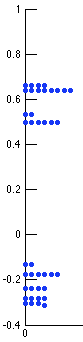
\includegraphics[height=150px]{Fig/Plots/r3a.png}
		\caption{}
	\end{subfigure}
	\begin{subfigure}{60px}
		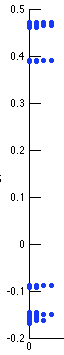
\includegraphics[height=150px]{Fig/Plots/r5b.png}
		\caption{}
	\end{subfigure}    
	\begin{subfigure}{60px}
		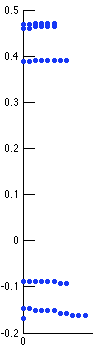
\includegraphics[height=150px]{Fig/Plots/r5a.png}
		\caption{}
	\end{subfigure}
	\caption{Energy levels for different sized QDs: 2nm (a), 6nm (b) and (c), 10nm (d) and (e). Vertical axis in eV. Multiple dots on the horizontal axis signify degeneracy. In plots (c) and (e) energies within 0.03eV are plotted as degenerate, for better visibility.}
	\label{fig:e-levels}	
\end{figure}

\begin{figure}
	\centering
	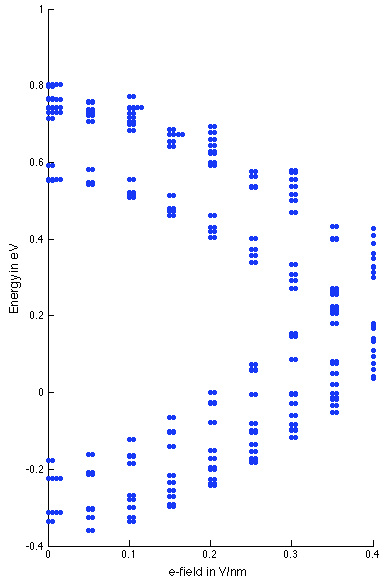
\includegraphics[width=200px]{Fig/Plots/r25v.png}
	\caption{Energy states (including degeneracy) for different electric fields.}
	\label{fig:EvsVolt}
\end{figure}


% TEXT
\begin{REMARK}
In the following discussion, the terms conduction band, band edge and so on are used. Although there are no energy bands present in a QD, but rather discrete energy levels, these terms nevertheless make sense, since the states above the band gap are similar to conduction band states, and those below to valence band states, respectively. Indeed, if the QD gets bigger, we finally reach the limit where we can treat it as a bulk material. The term \textit{conduction band} refers in this context to the discrete energy states above the band gap.
\end{REMARK}
	
Taking a look at the eigenenergies close to the bandedge, one can see that there are 8 closely spaced modes, for conduction and valence band respectively. Generally, closest to the band edge there is a twofold degenerate energy level, followed by a fourfold degenerate level and then again a twofold degenerate level. (For a few simulations the order is different, for example the fourfold degenerate energy level is closest to the band edge.)
	
As the size of the QDs increases, the energy levels get closer to each other, resulting in higher degeneracy. This is shown in figure~\ref{fig:e-levels} (a),(b),(d), where the energy levels (including degeneracy) are shown for 2, 6 and 10nm QDs. Since some levels are very closely spaced, they are not clearly distinguishable form each other. For this reason, the tolerance, within which an energy level is shown as degenerate, was increased in figure~\ref{fig:e-levels} (c),(e). An effective eightfold degeneracy for the 10nm QD is now clearly visible.
	
In the presence of an electric field, this degeneracy is broken, leading to more energy levels, which are all, interestingly, twofold degenerate. This is shown in figure~\ref{fig:EvsVolt} for a 5nm QD, where the energy levels are plotted against an applied electric field. One can clearly see how the band gap gets smaller, as is discussed later on.
\FloatBarrier

\section{Band gap} \label{sec:BandGapAnalysis}
	All band gaps of our PbS simulations are plotted in figure \ref{fig:BandGap}. Furthermore, we have fitted the $1/R^2$ dependence of
	equation \ref{eq:Bandgap} to all band gaps where no voltage was applied.
	As we can see from the graph, the bulk band gap of \gls{PbS} should approximately be 0.46eV, which means a pretty big deviation
	from experimentally determined values of 0.37eV at 302K (see appendix \ref{sec:PbS}). We have made the same observations while comparing
	other experimental values with simulation data. As experimental data, \gls{TEM} images, absorption and \gls{PL} spectra (see figure \ref{fig:PbS_TEM},
	\ref{fig:Abs_PbS} and \ref{fig:PL_PbS}) were available. From the \gls{TEM} images, average particle sizes were measured and compared
	with approximately equivalently sizes from simulations. The results are listed in table \ref{tbl:BandGap}. Significant deviations
	can be noticed between experimental and simulated data, which are reasoned in three significant error sources, that explain the deviations.
	First of all, the synthesis does not deliver perfect spherical and homogeneous \glspl{QD}, which causes the broadening of the spectra.
	Second: it is very difficult to determine the size of the \glspl{QD} from the \gls{TEM} images, especially without
	sophisticated software. This might lead to comparison of experimental and simulated values, which actually do not belong to each other.
	Third: comparing measurements of the real physical world with simulations. There might be errors in the measurement
	apparatus, impurities in the \glspl{QD} and disregarded effects in the simulation, which have an impact in reality.
	
	\begin{table}[t]
		\centering
		\begin{tabularx}{\textwidth}{Xc|c|c|c}
															& \multicolumn{4}{c}{Experimental \diameter - Simulated \diameter}														\\
															&	$\sim$ 2.97nm	- 3nm		&	$\sim$ 3.21nm - 3nm &	$\sim$ 3.95nm	-	4nm		&	$\sim$ 4.97nm - 5nm		\\
															&	PbS - 261				& PbS - 61						&	PbS - 190							&	PbS - 220							\\
			\hline
			Energy at \gls{PL} peak	&	1.4529eV 							&	1.2256eV 						&	n/a										&	1.0040eV 							\\
															&	(853nm)								&	(1012nm)						&												&	(1235nm)							\\
			Band gap experimental		&	1.7487eV 							&	1.5194eV 						&	1.2808eV 							&	1.0489eV 							\\
															&	(709nm)								&	(816nm)							&	(968nm)								&	(1182nm)							\\
			Band gap simulated			&	0.9929eV							&	0.9929eV						&	0.8645eV							&	0.7296eV							\\ \\
		\end{tabularx}
		\caption{Comparison of experimental and simulated band gaps.}
		\label{tbl:BandGap}
	\end{table}
	
	\begin{figure}[t]
		\centering
		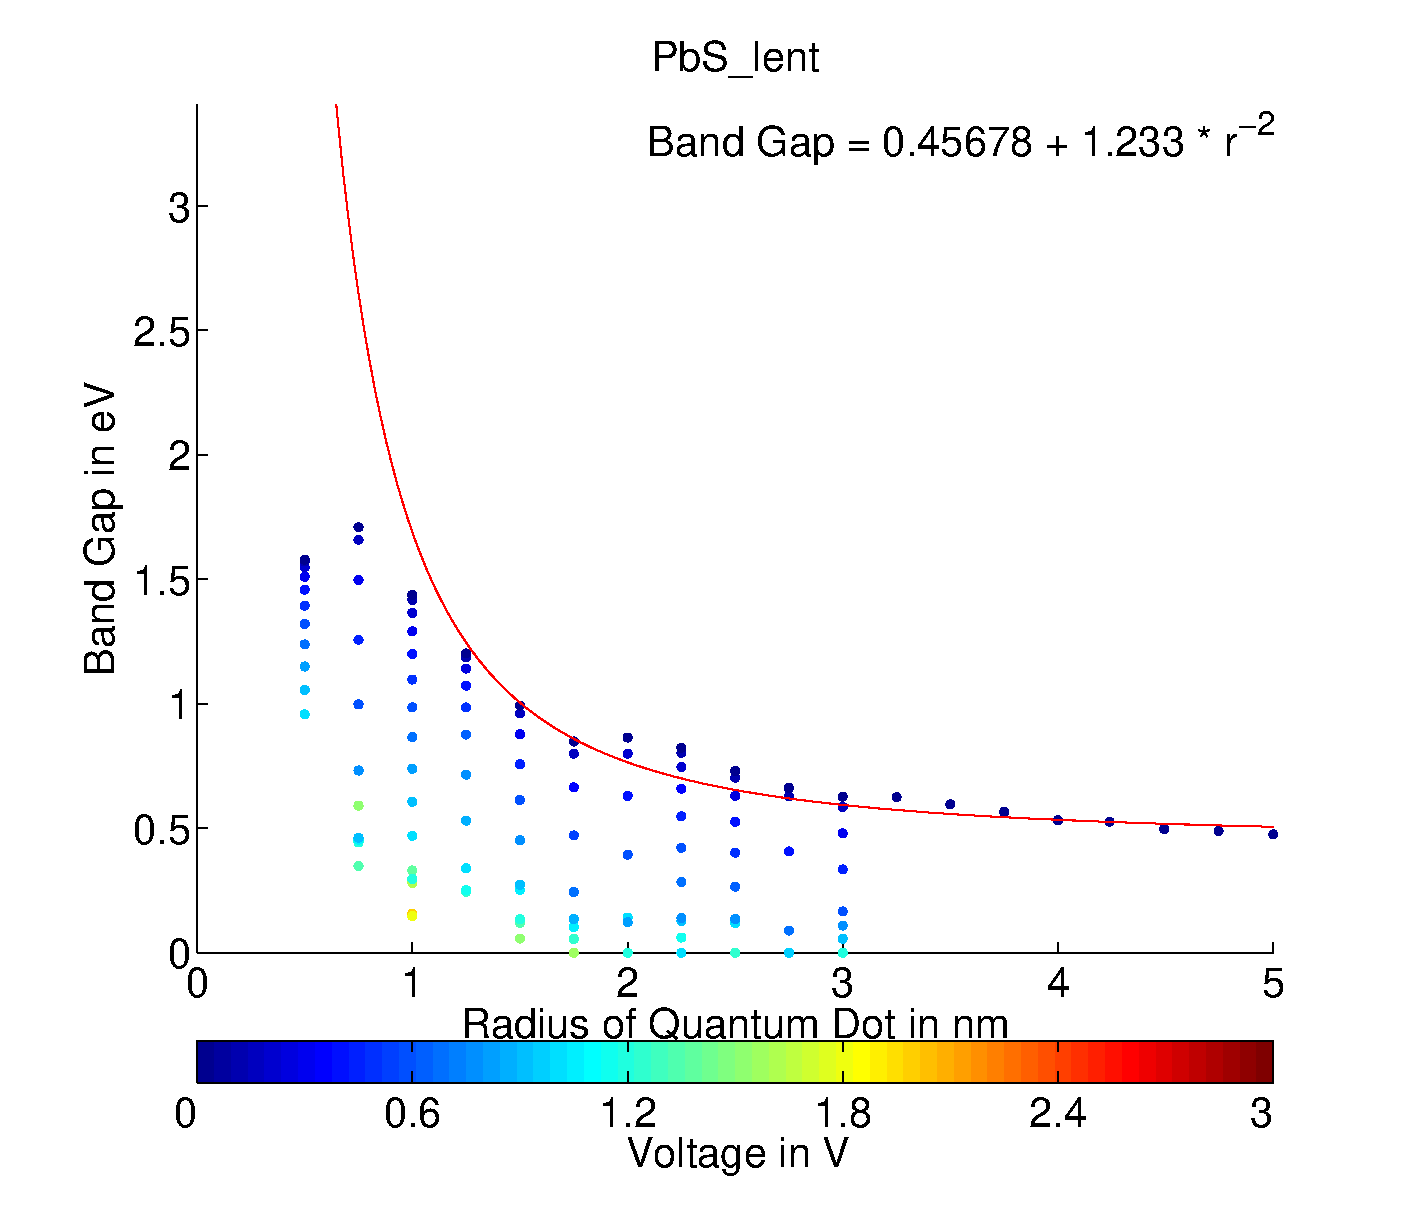
\includegraphics[width=0.8\textwidth]{Fig/Plots/BandGap.eps}
		\caption{PbS band gaps against radius of all simulated \glspl{QD}. The color indicates the applied voltage.}
		\label{fig:BandGap}
	\end{figure}
	
	\begin{figure}[htpb]
		\centering
		\begin{subfigure}{0.23\textwidth}
			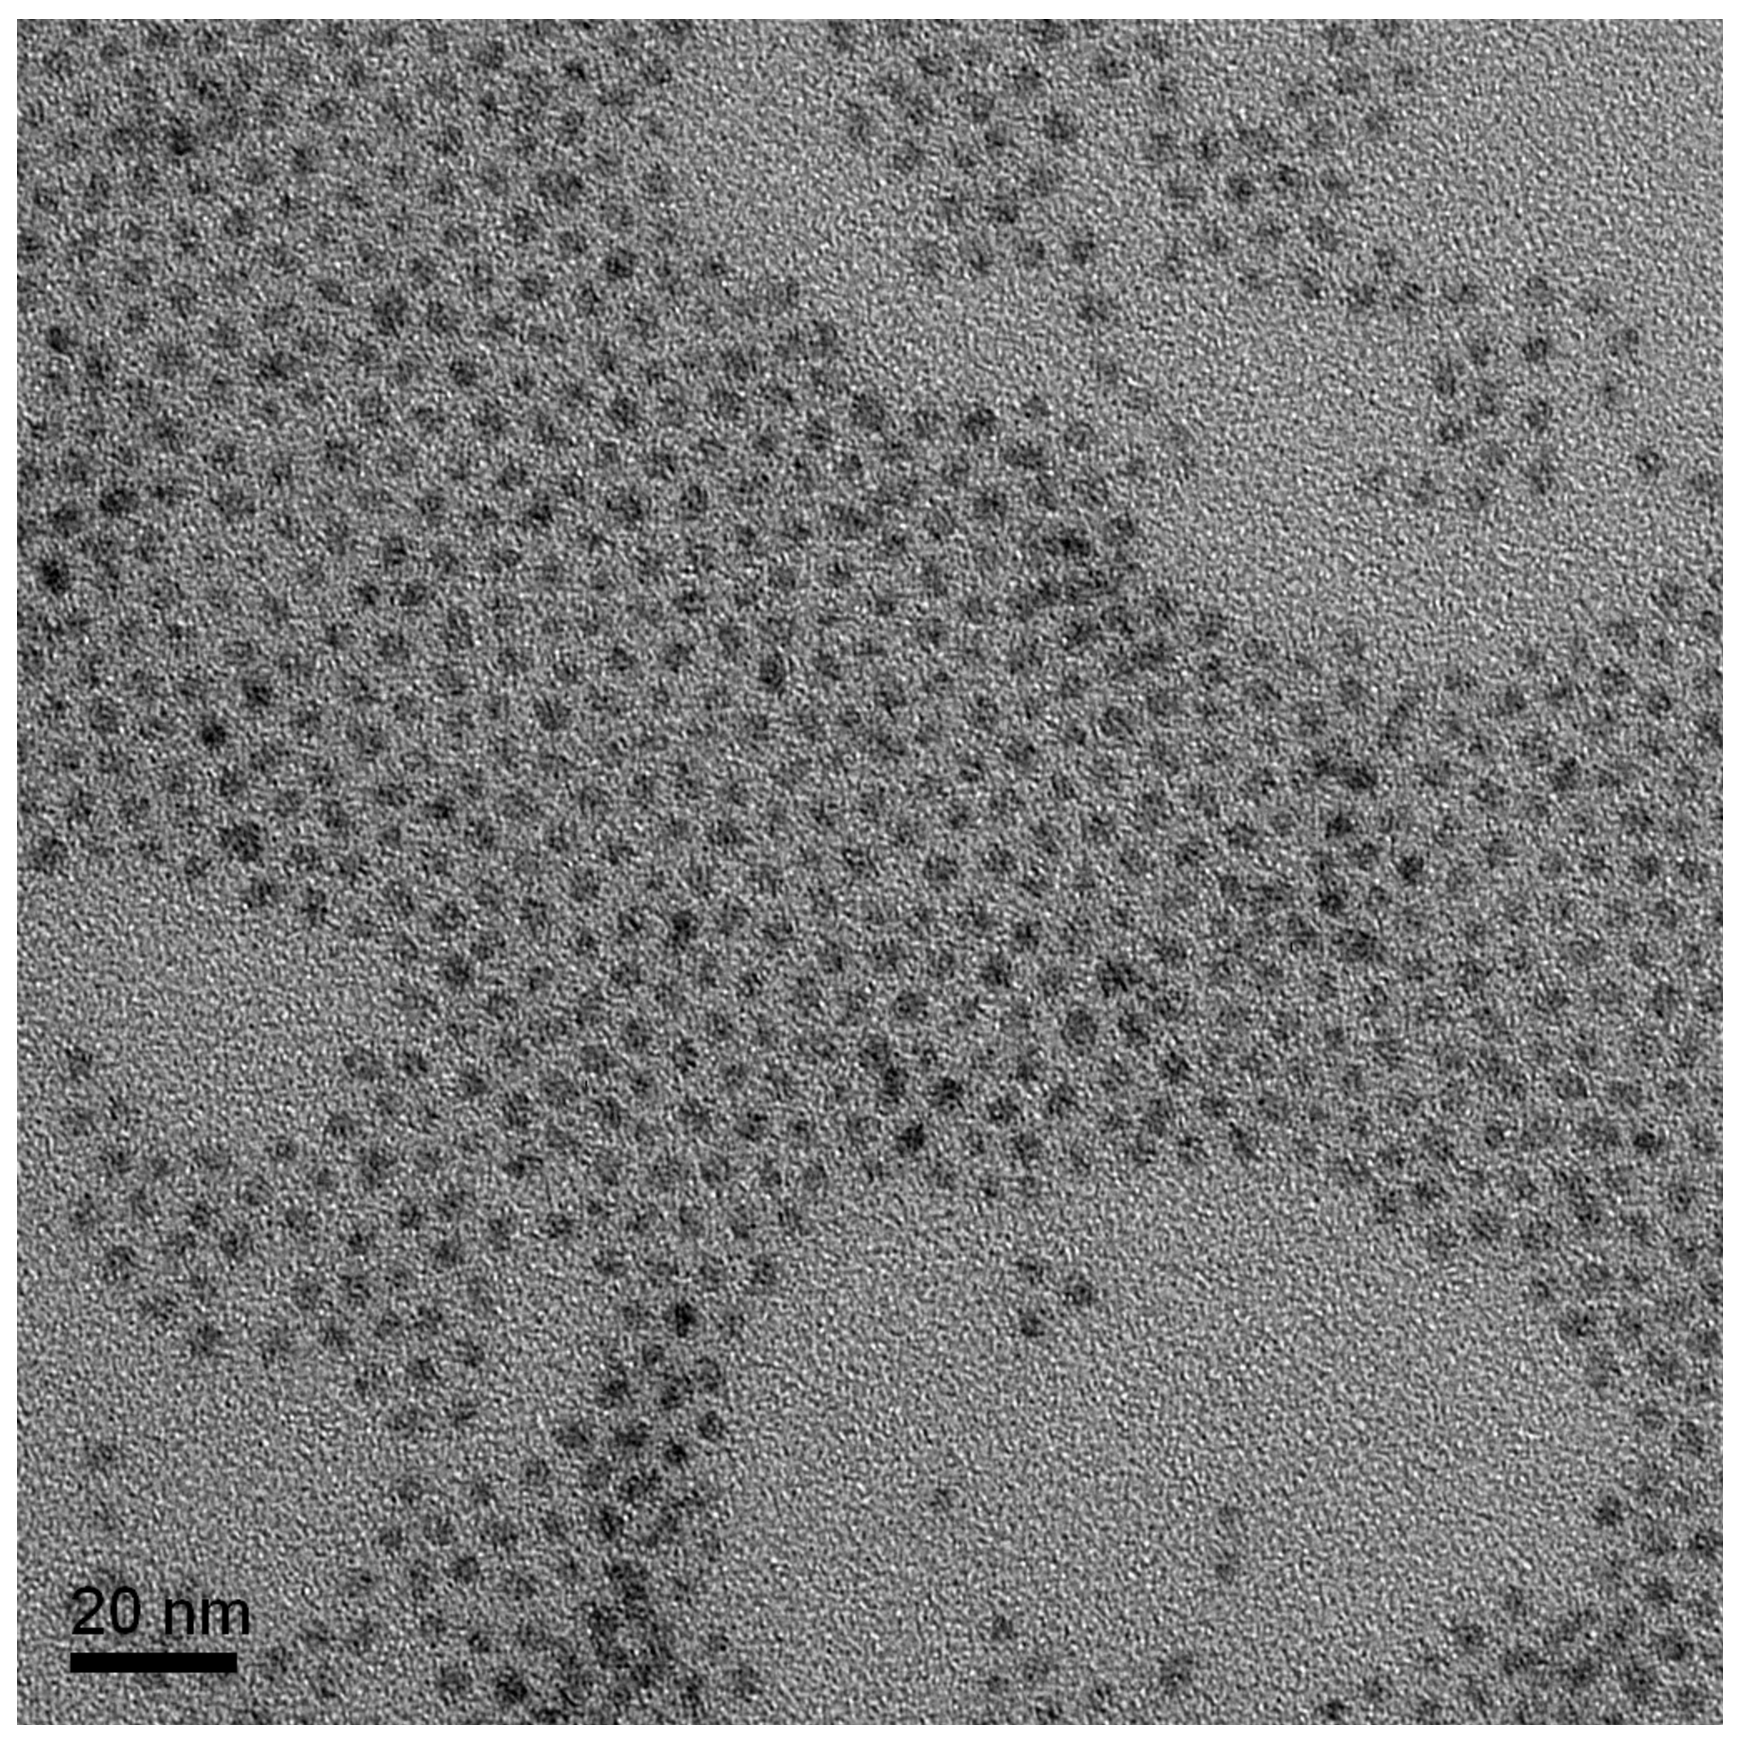
\includegraphics[width=\textwidth]{Fig/Plots/PbS_190_TEM.eps}
			\caption{PbS - 190, \diameter $\sim$ 3.95nm}
		\end{subfigure}
		\hfill   
		\begin{subfigure}{0.23\textwidth}
			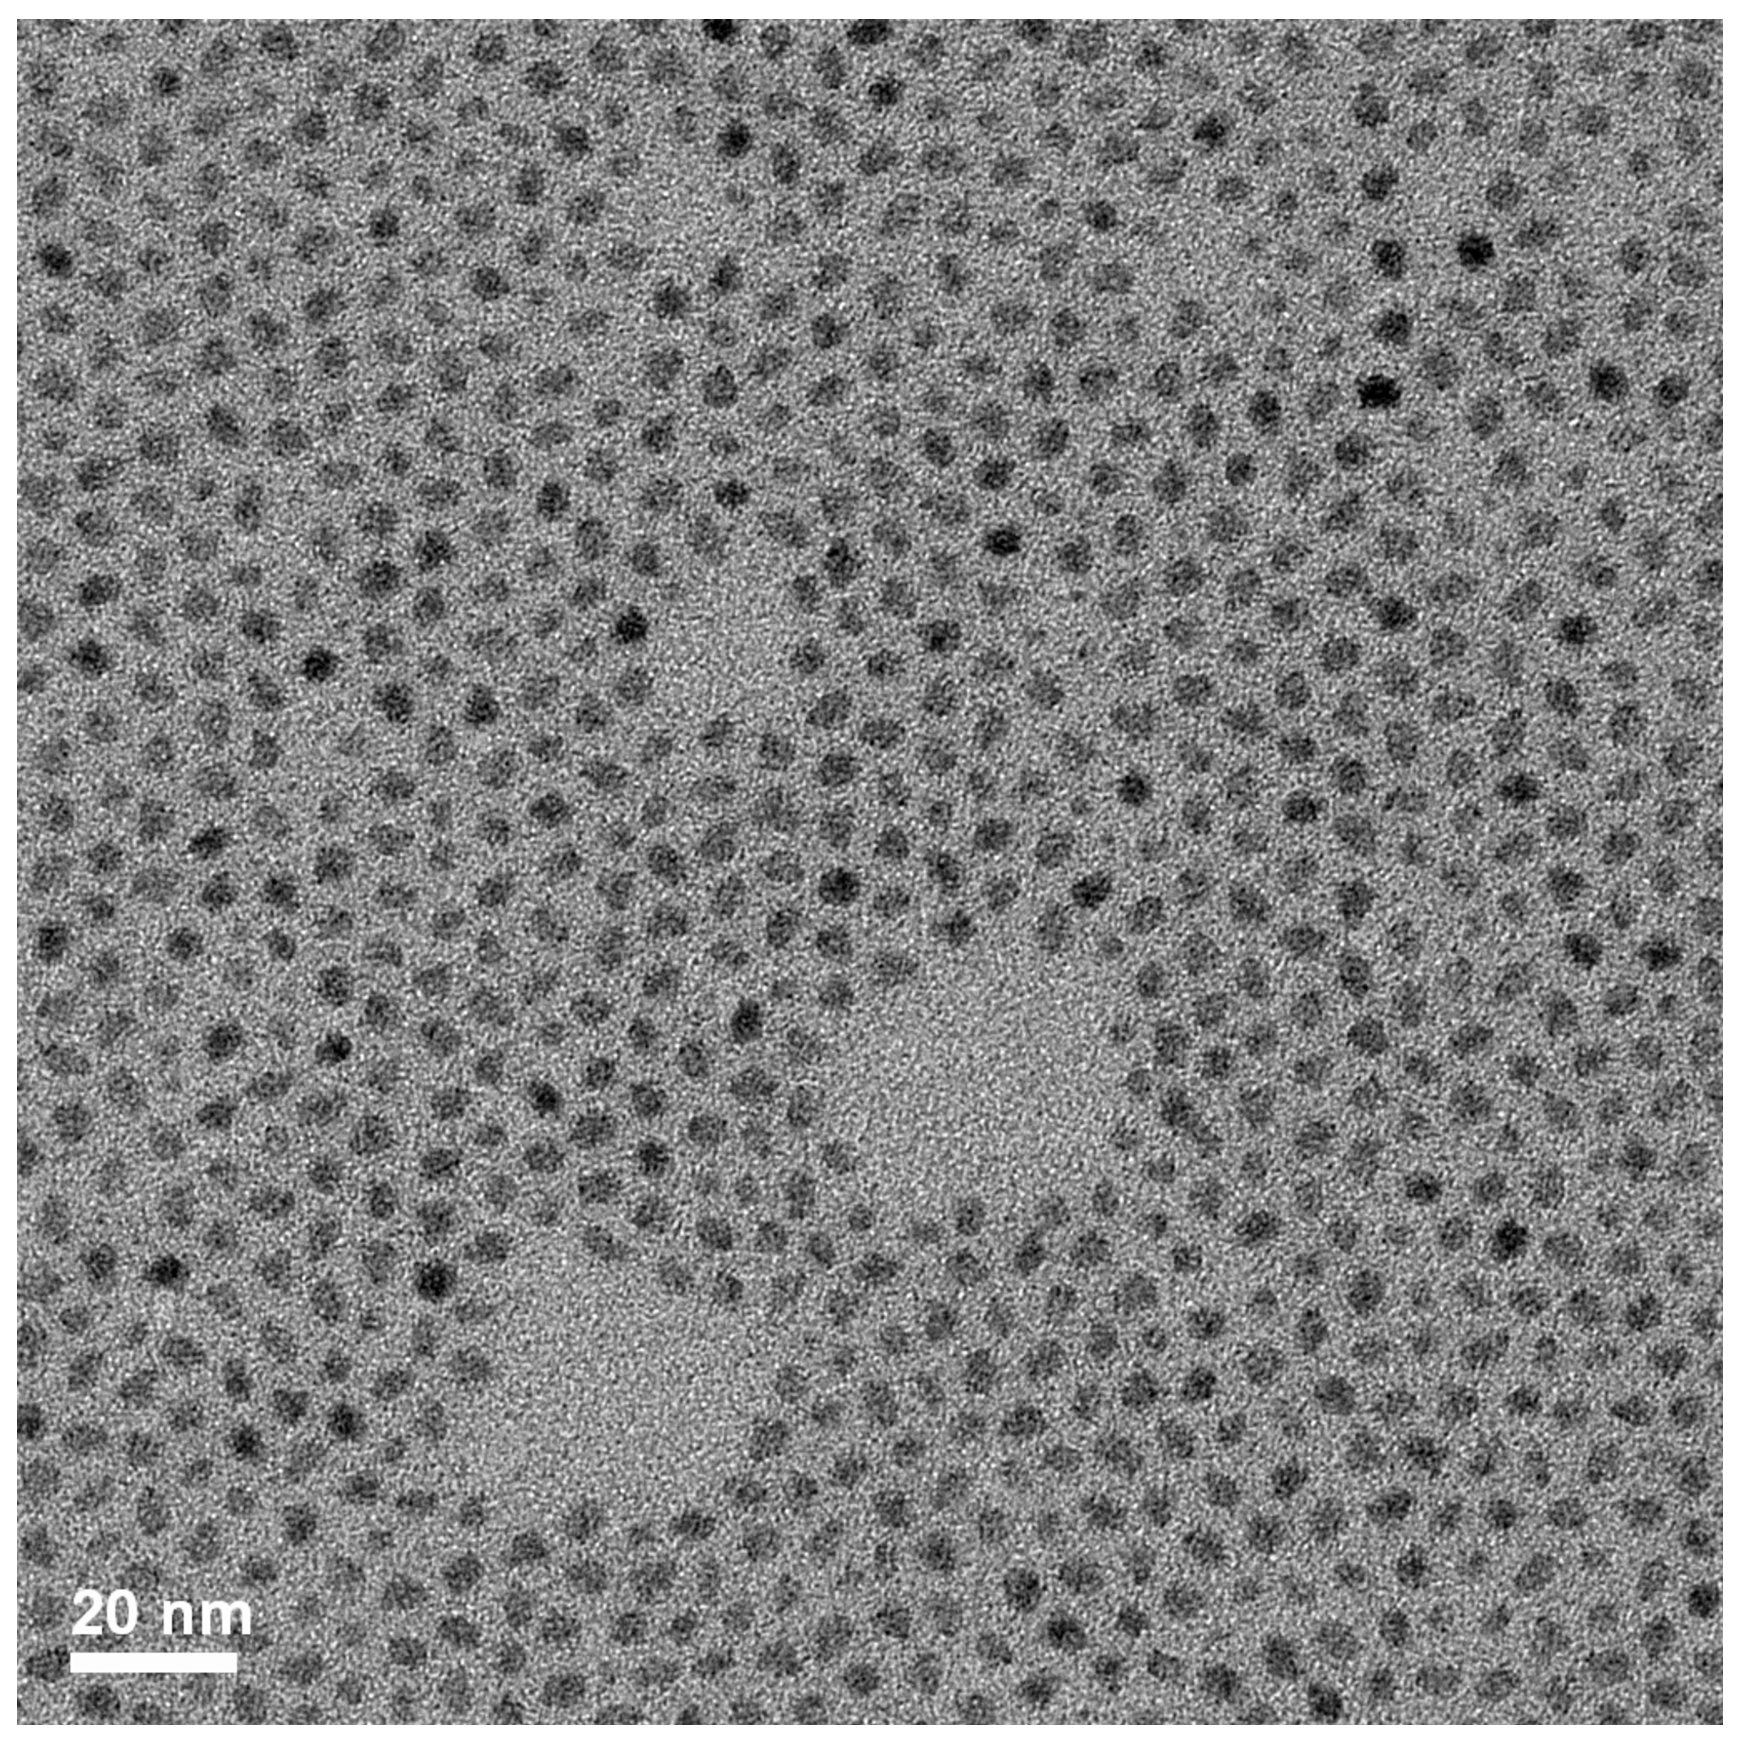
\includegraphics[width=\textwidth]{Fig/Plots/PbS_220_TEM.eps}
			\caption{PbS - 220, \diameter $\sim$ 4.97nm}
		\end{subfigure}
		\hfill
		\begin{subfigure}{0.23\textwidth}
			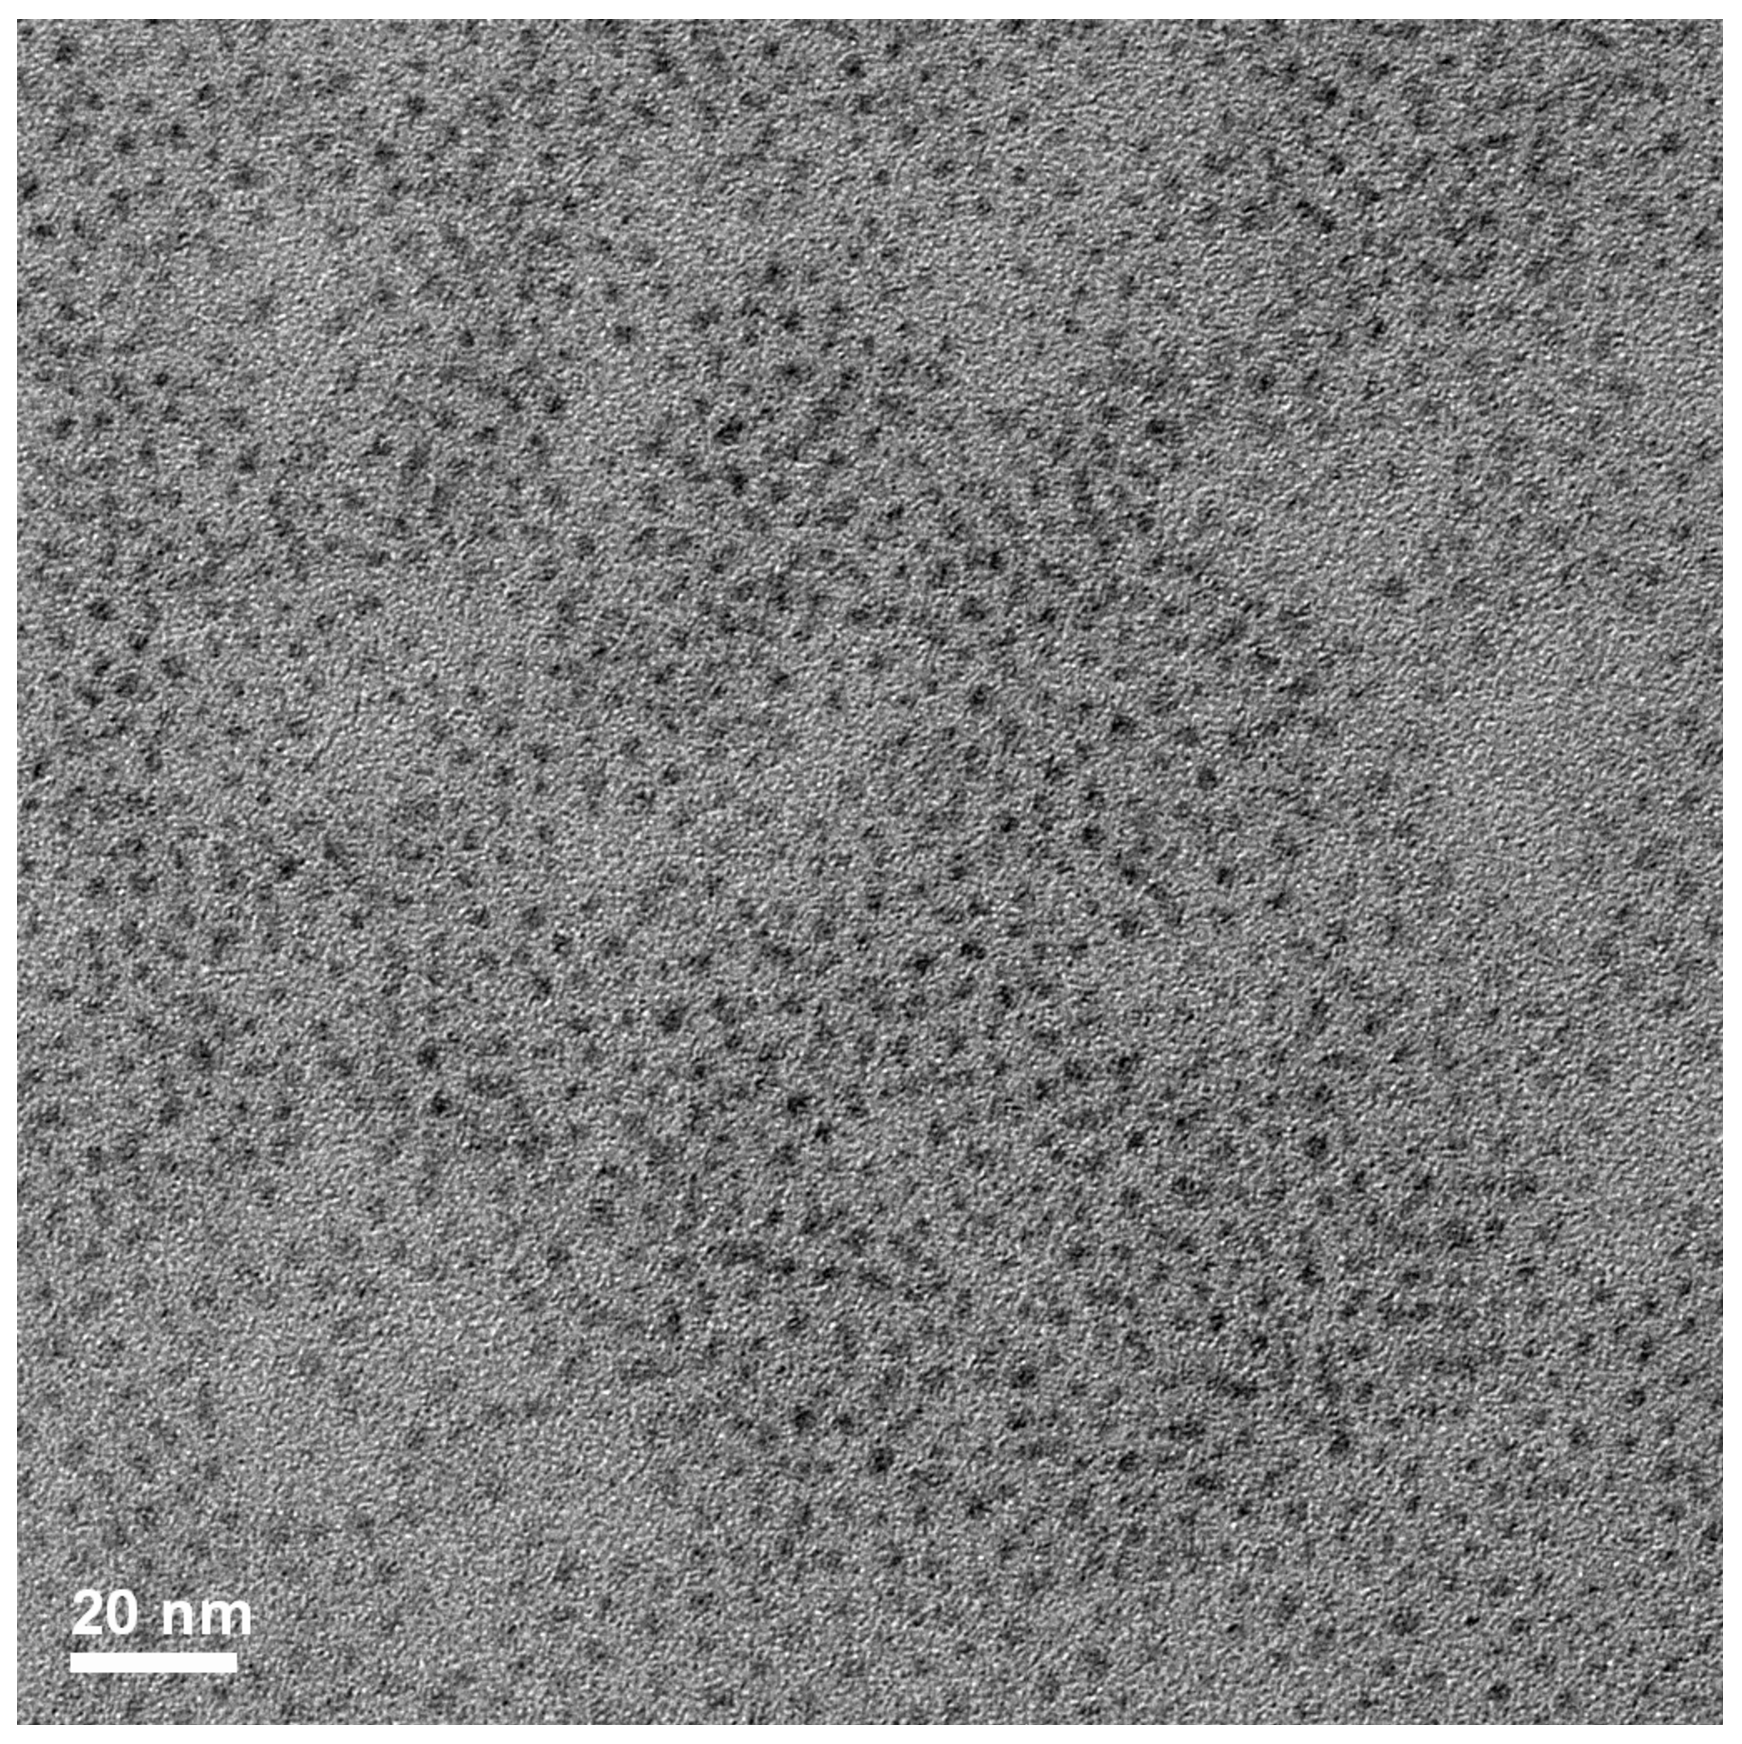
\includegraphics[width=\textwidth]{Fig/Plots/PbS_261_TEM.eps}
			\caption{PbS - 261, \diameter $\sim$ 2.97nm}
		\end{subfigure}
		\hfill
		\begin{subfigure}{0.23\textwidth}
			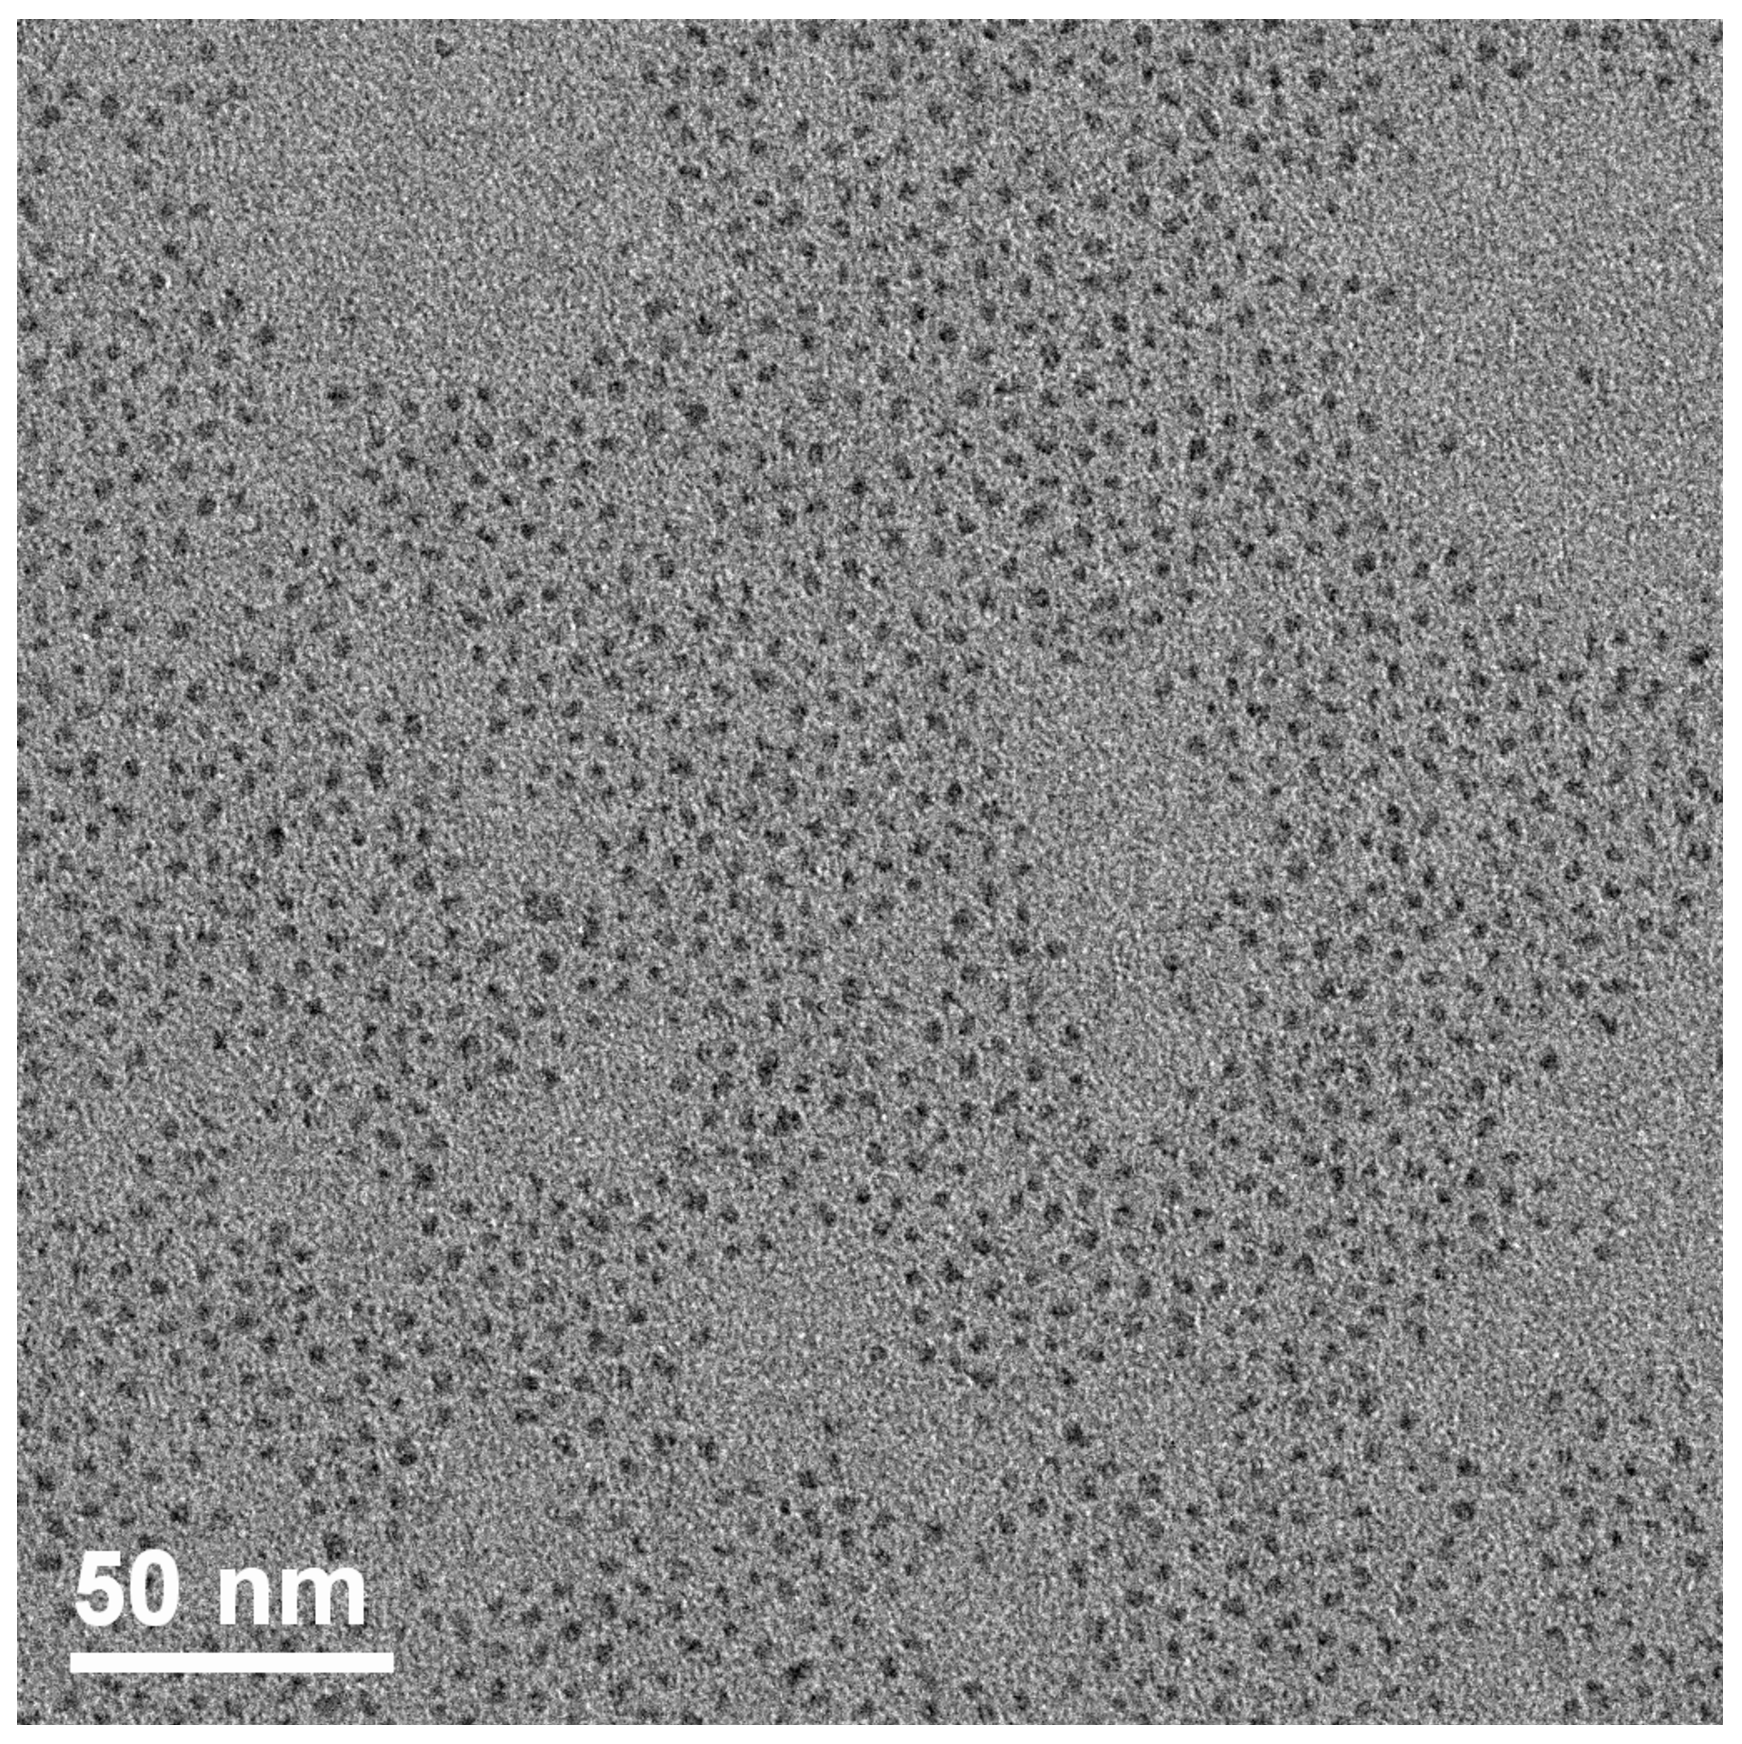
\includegraphics[width=\textwidth]{Fig/Plots/PbS_61_TEM.eps}
			\caption{PbS - 61, \diameter $\sim$ 3.21nm}
		\end{subfigure}
		\caption{\gls{TEM} images of PbS \glspl{QD}}
		\label{fig:PbS_TEM}	
	\end{figure}

	\begin{figure}[htpb]
		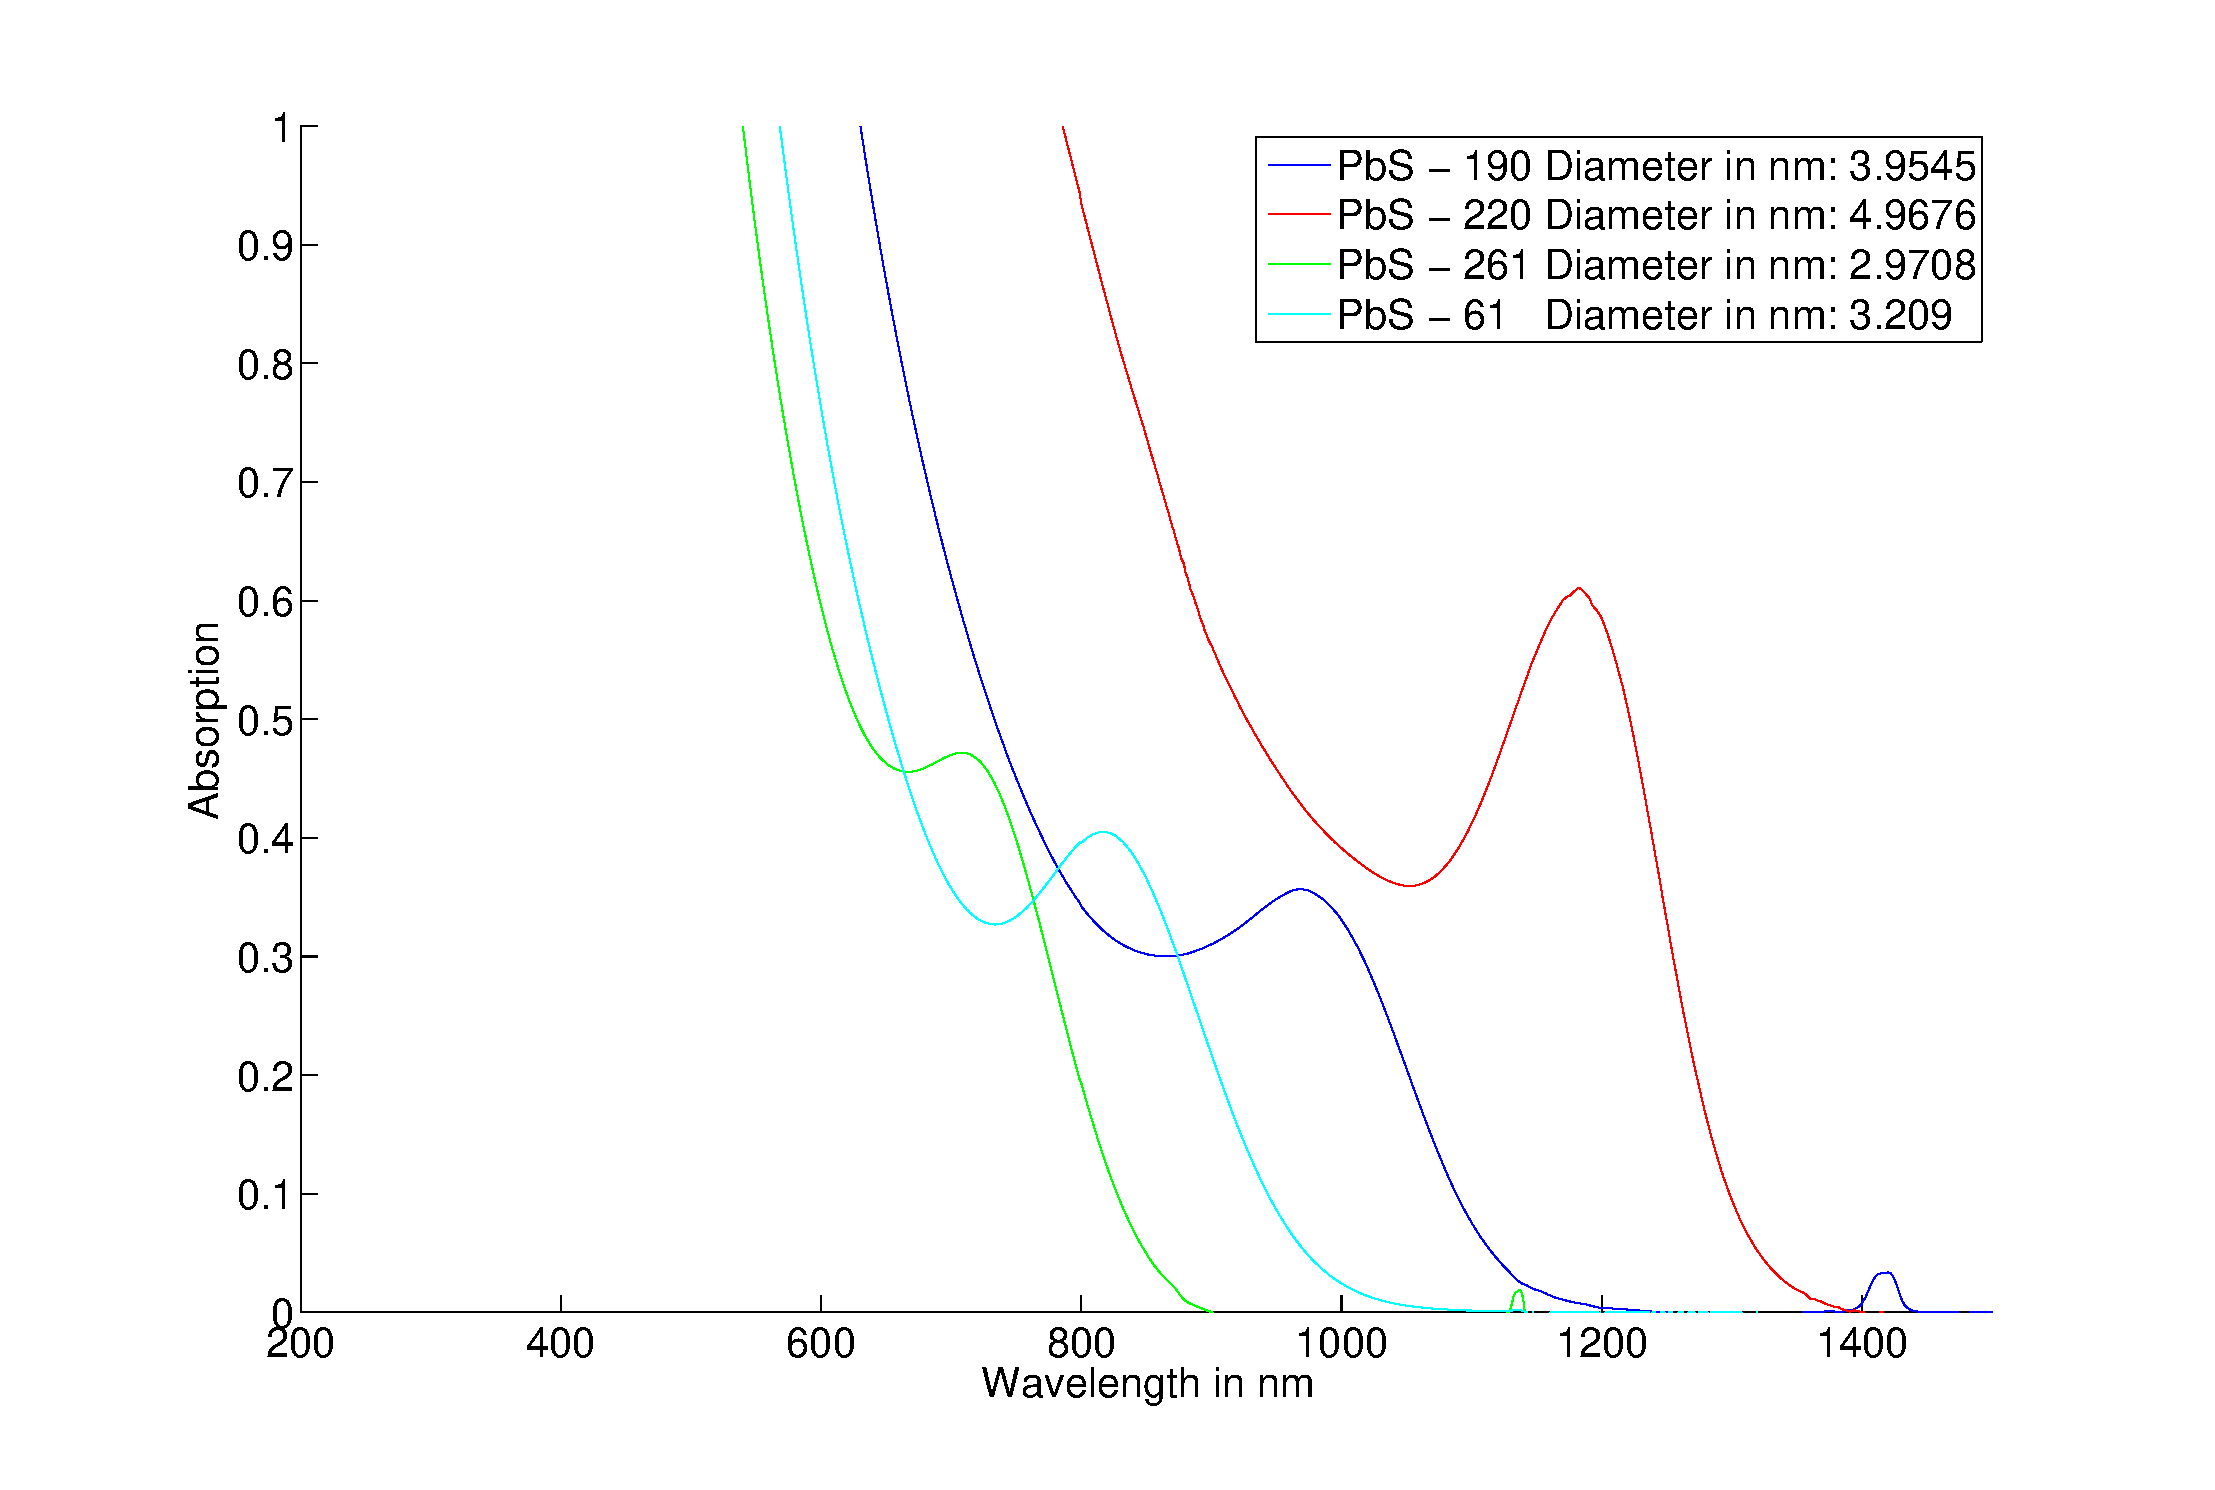
\includegraphics[width=\textwidth]{Fig/Plots/Abs_PbS.eps}
		\caption{Experimentally determined absorption, plotted against wavelength in nm for 4 synthesized PbS \glspl{QD}.}
		\label{fig:Abs_PbS}
	\end{figure}
	
	\begin{figure}
		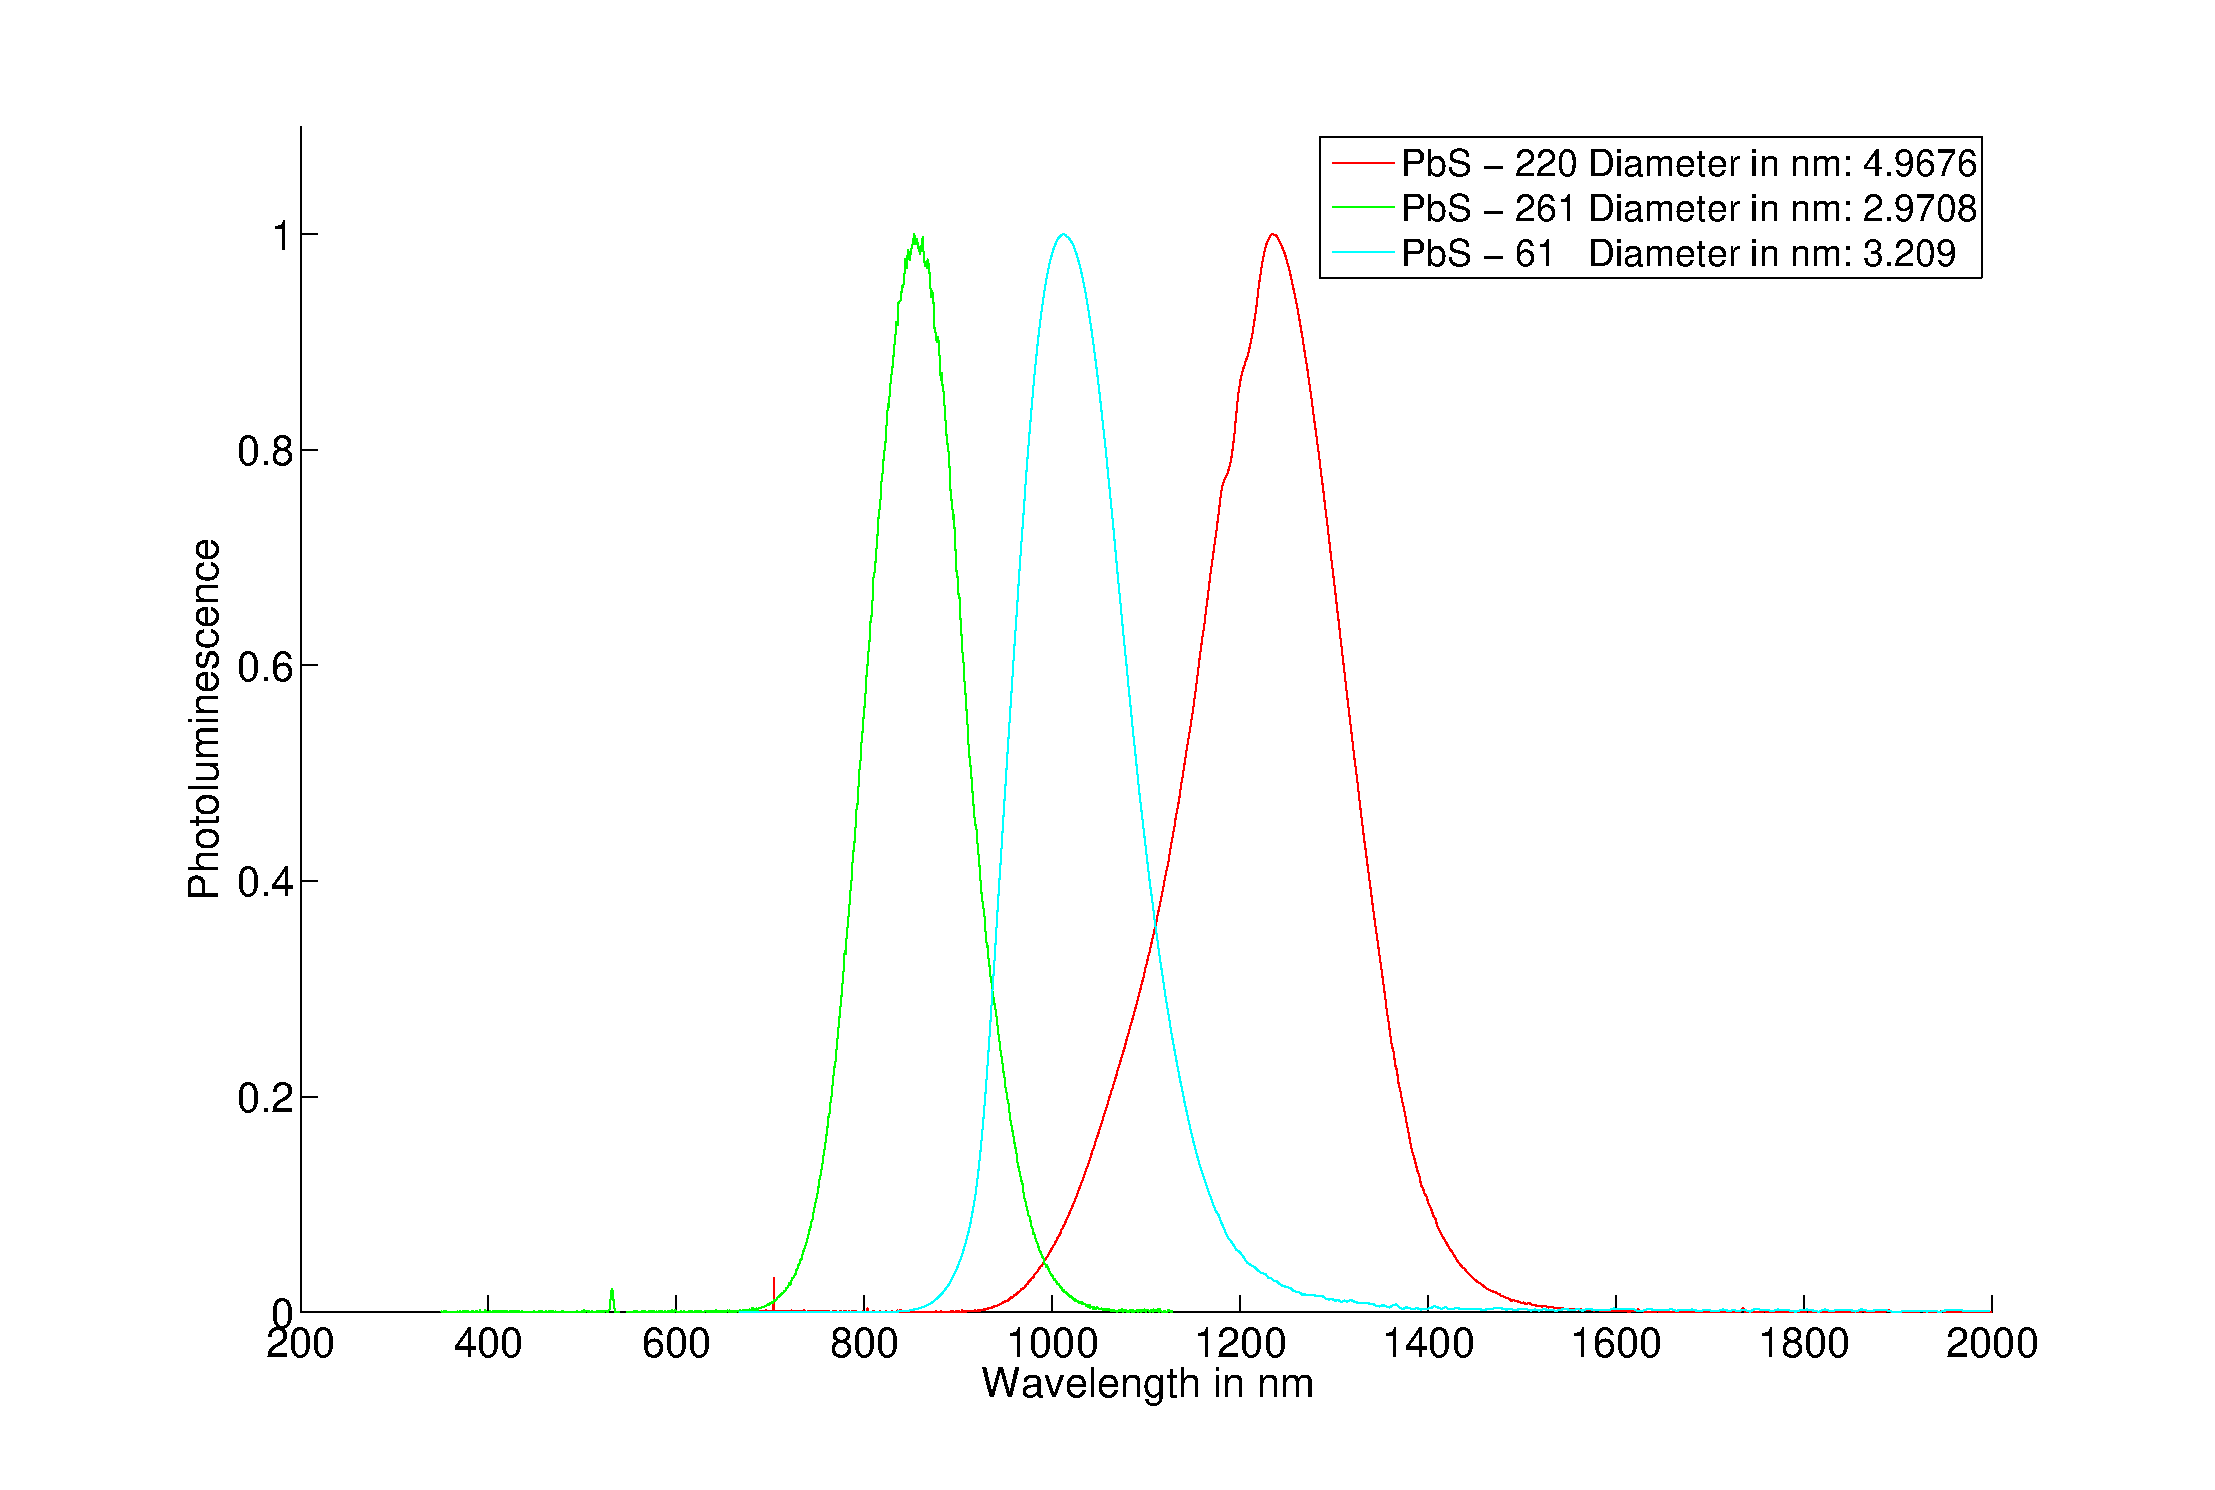
\includegraphics[width=\textwidth]{Fig/Plots/PL_PbS.eps}
		\caption{Experimentally determined \gls{PL} plotted against wavelength in nm for 3 synthesized PbS \glspl{QD}.}
		\label{fig:PL_PbS}
	\end{figure}
		
	\begin{REMARK}
		All experimental data used in this section were provided by the \gls{LNE} at ETH Zurich.
	\end{REMARK}

\newpage
\subsection{Band gap of QDs with an applied voltage}
	In figure \ref{fig:EnergyLevels_Volt} we can see, that with increasing voltage the band gaps approach a zero value. Interestingly, this does not happen linearly, 
	for every constant voltage increment. By visualizing this effect for constant radii (figure \ref{fig:BandGap_Volt}), we recognize that the energy gap drops
	in a	parabolic way until it completely reaches the zero value. Furthermore, we recognize in figure \ref{fig:EnergyLevels_Volt} a shift of all energy 
	levels towards each other.
	\begin{figure}
		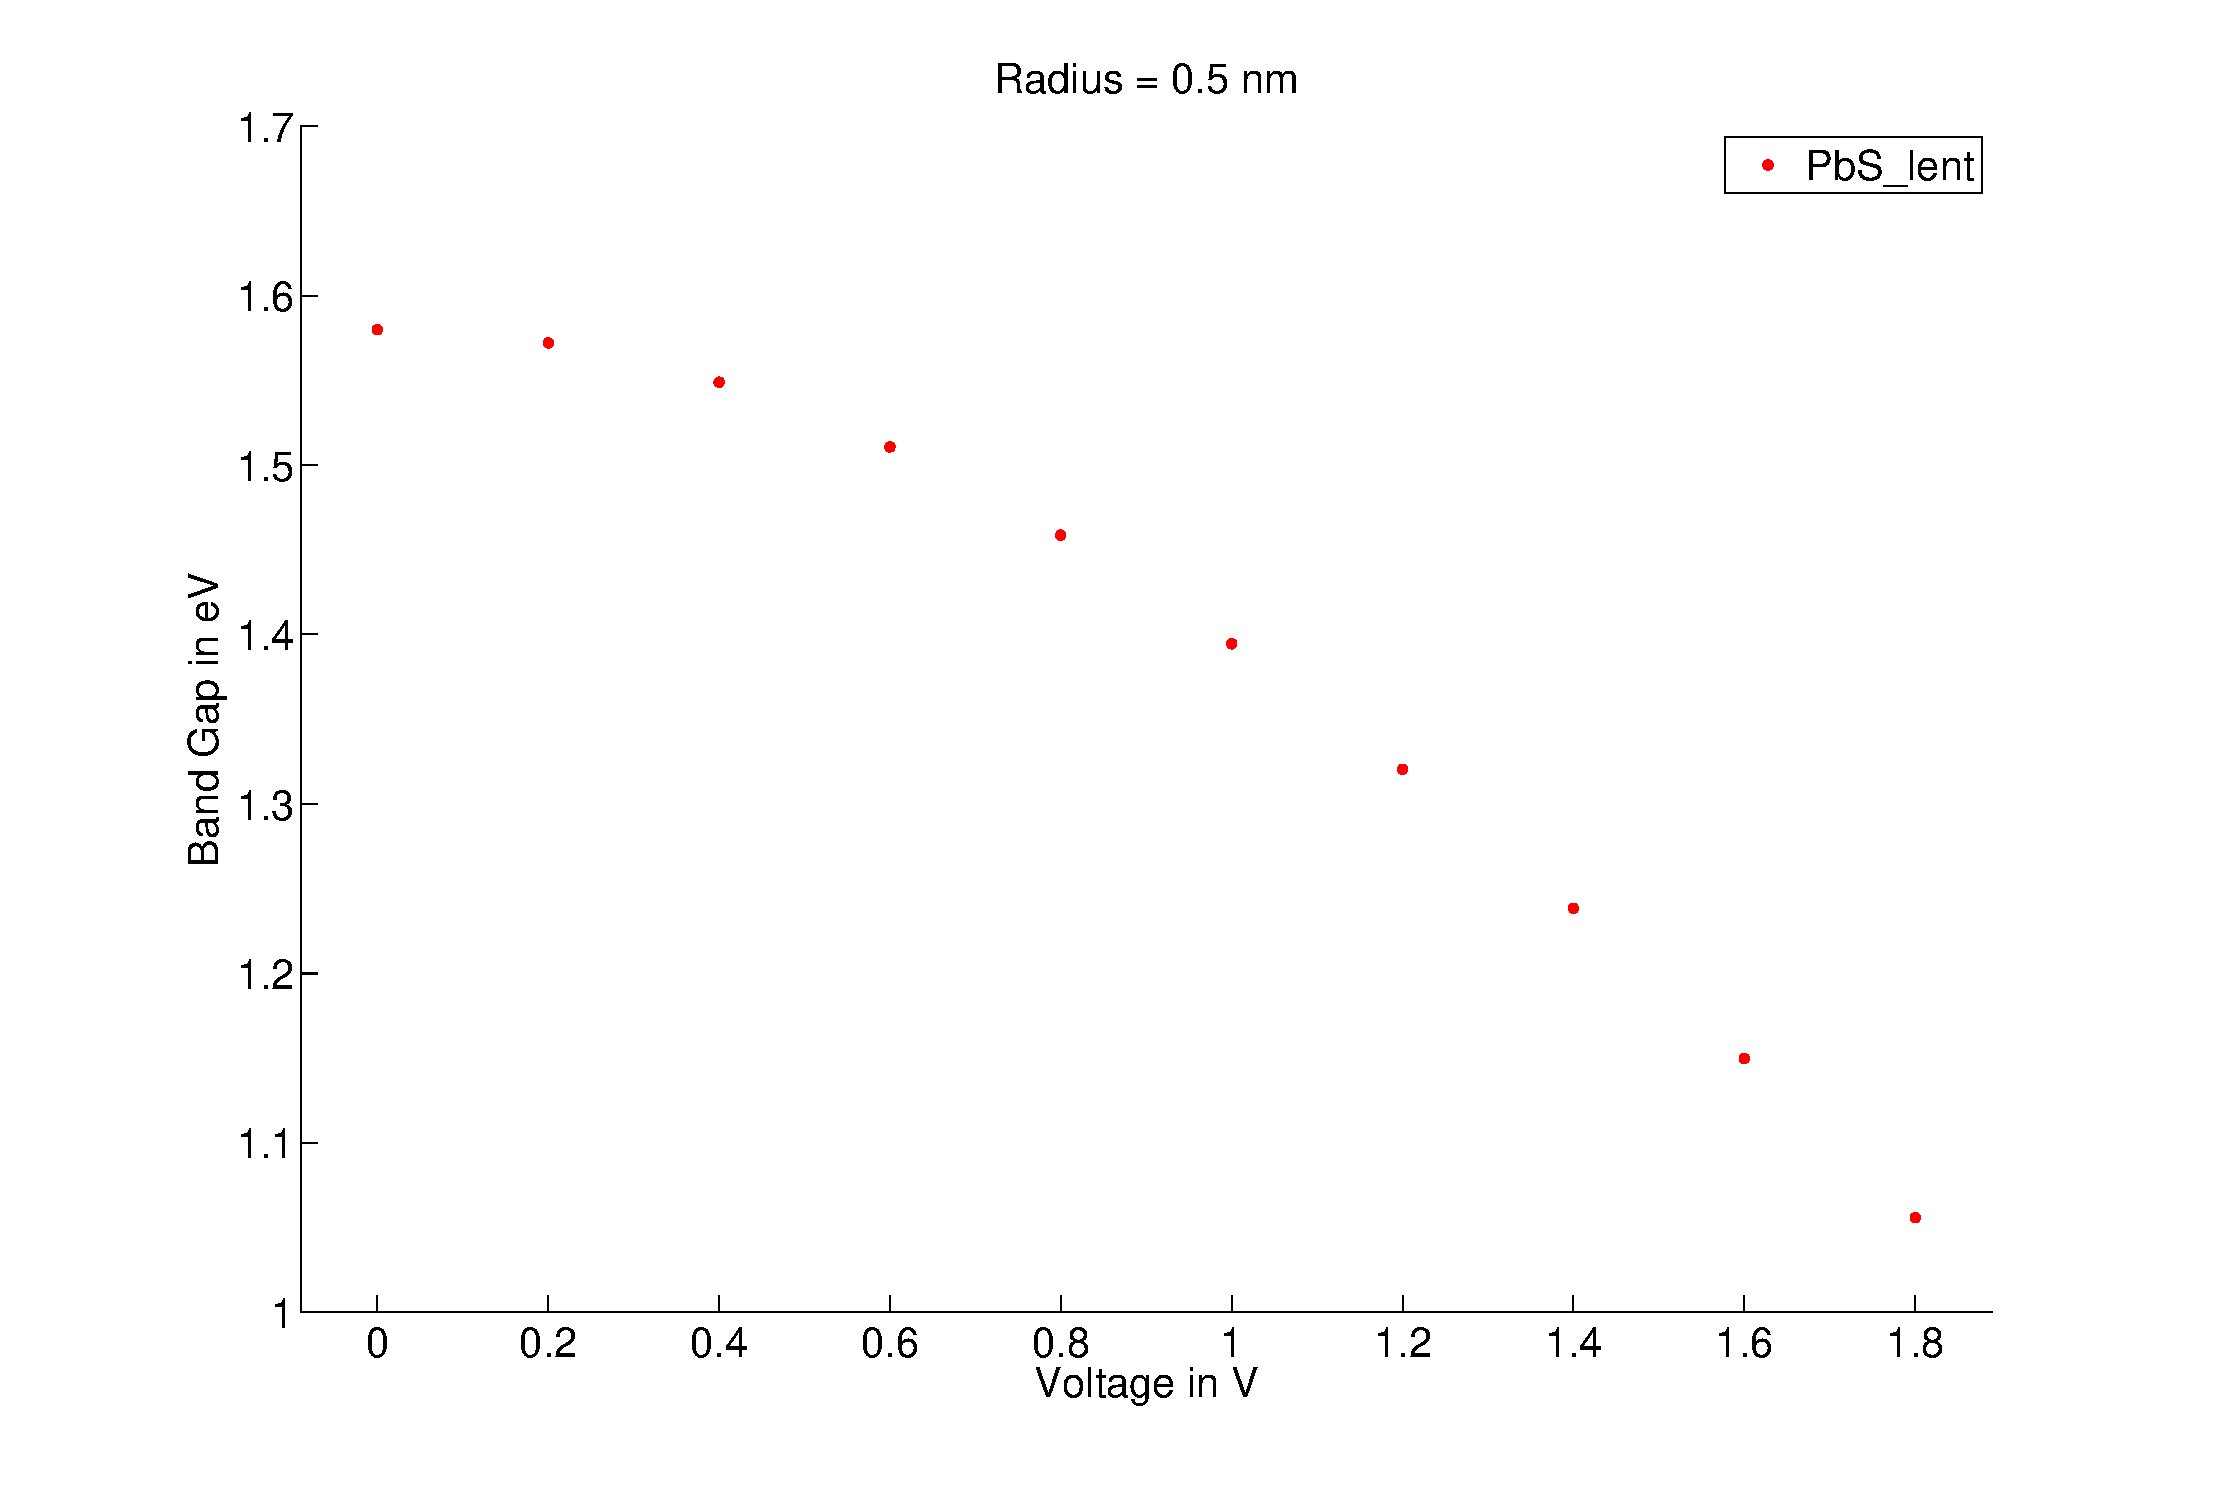
\includegraphics[width=\textwidth]{Fig/Plots/BandGap_Volt.eps}
		\caption{PbS band gaps plotted against voltage with constant radius 0.5nm.}
		\label{fig:BandGap_Volt}
	\end{figure}
	\begin{figure}
		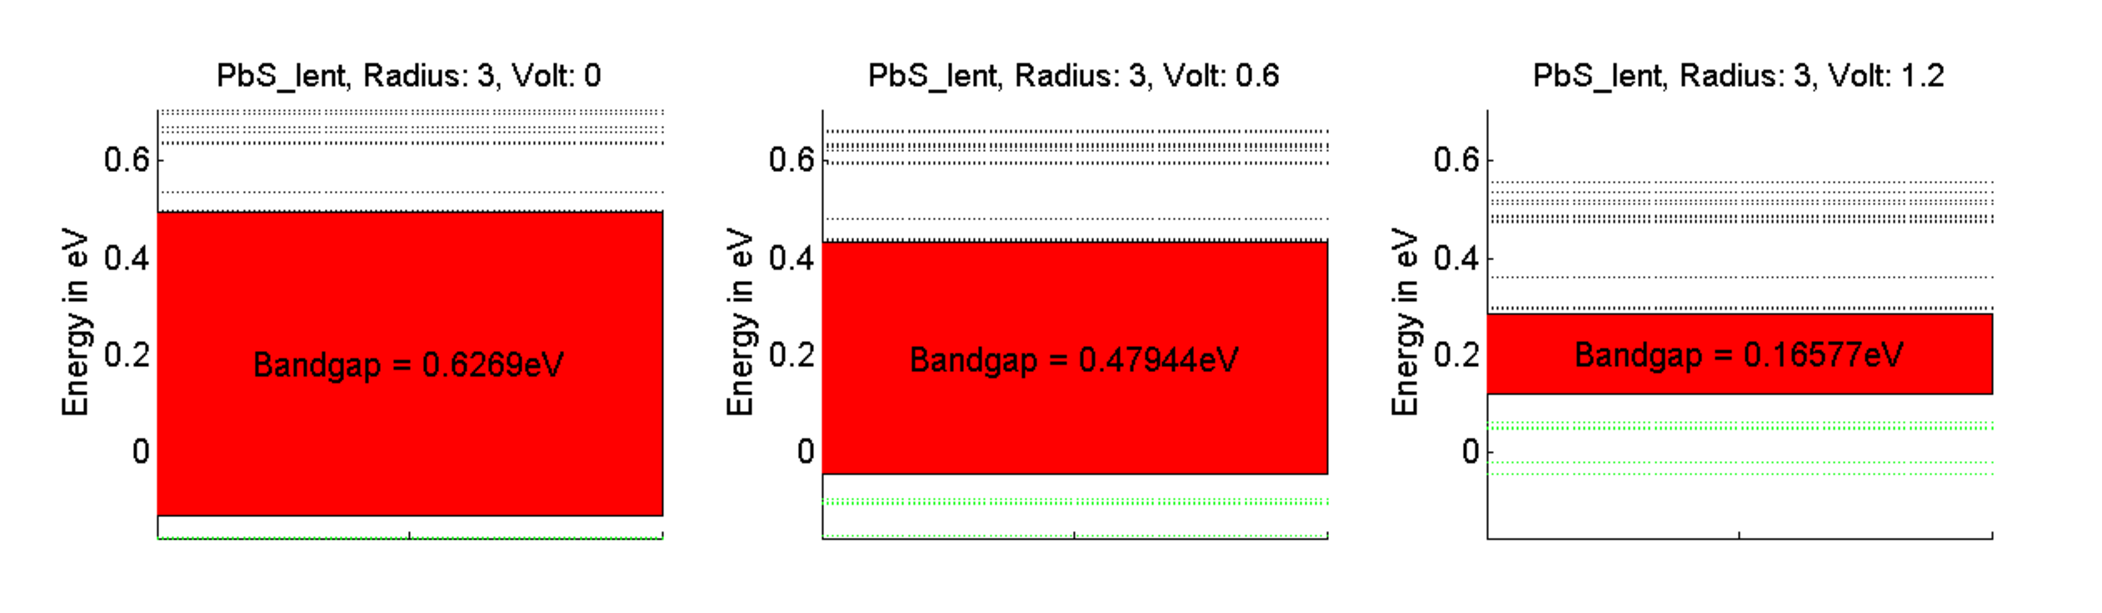
\includegraphics[width=\textwidth]{Fig/Plots/EnergyLevels.eps}
		\caption{PbS energy levels for different voltages with constant radius 3nm.}
		\label{fig:EnergyLevels_Volt}
	\end{figure}
	
\section{Wave functions}
% WAVE FUNCTIONS 

\subsection{Shape of the wave functions}

\subsubsection{QDs bigger than 3nm} 

% FIGURES
\begin{figure}[htbp]
	\centering
	\includegraphics[width=200px]{Fig/Plots/r4CBMod6}
	\caption{Probability density for an energy state in the lower conduction band of an 8nm QD. Locations of very high probability are shown in red, those of medium to high probability in yellow, such that the sum of the probabilities of all yellow and red locations is 50\%. Note that in following figures, different probability values may be used, for better visibility.}
	\label{fig:sphericalWaveFn}
\end{figure}
%
\begin{figure}[htbp]
	\centering
	\begin{subfigure}{150px}
		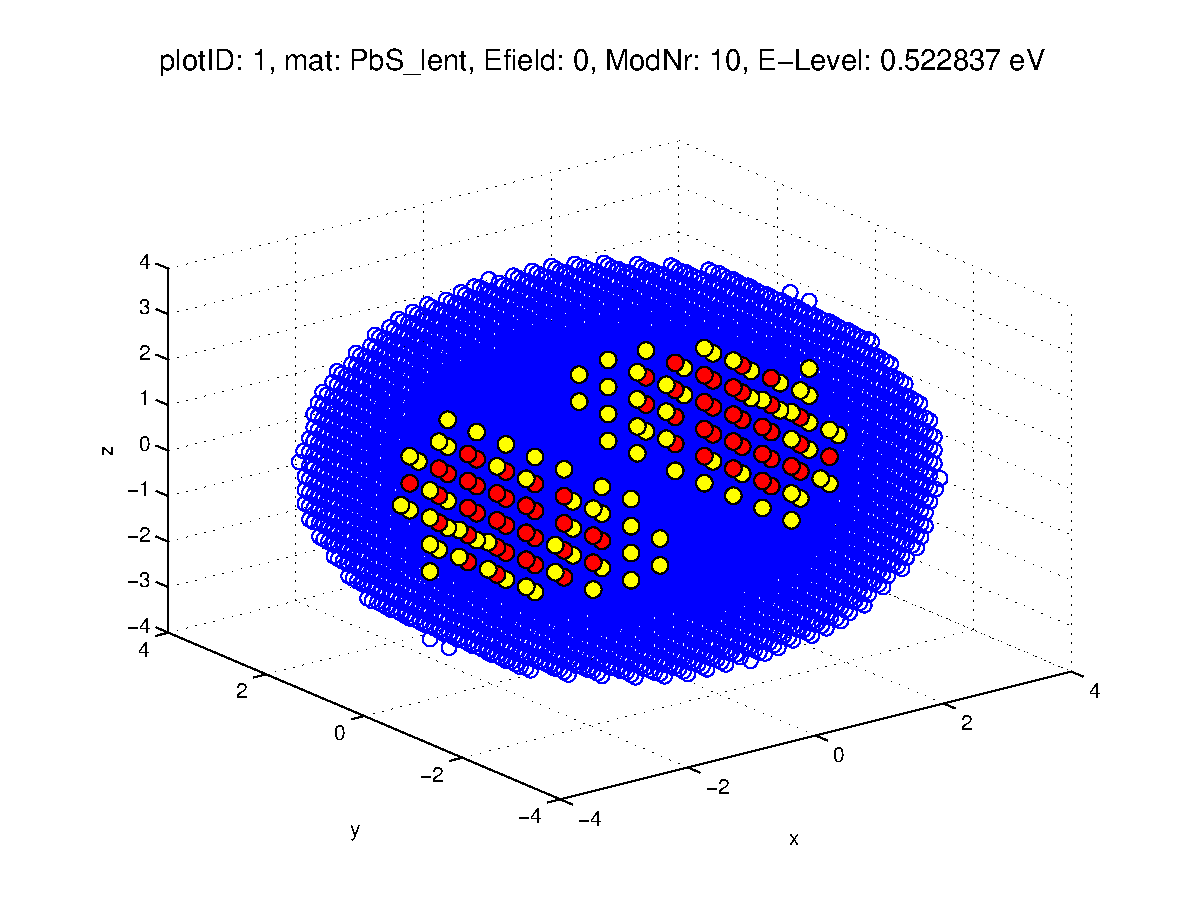
\includegraphics[width=150px]{Fig/Plots/r4CBmod10}
		\caption{}
	\end{subfigure}
	\begin{subfigure}{150px}
		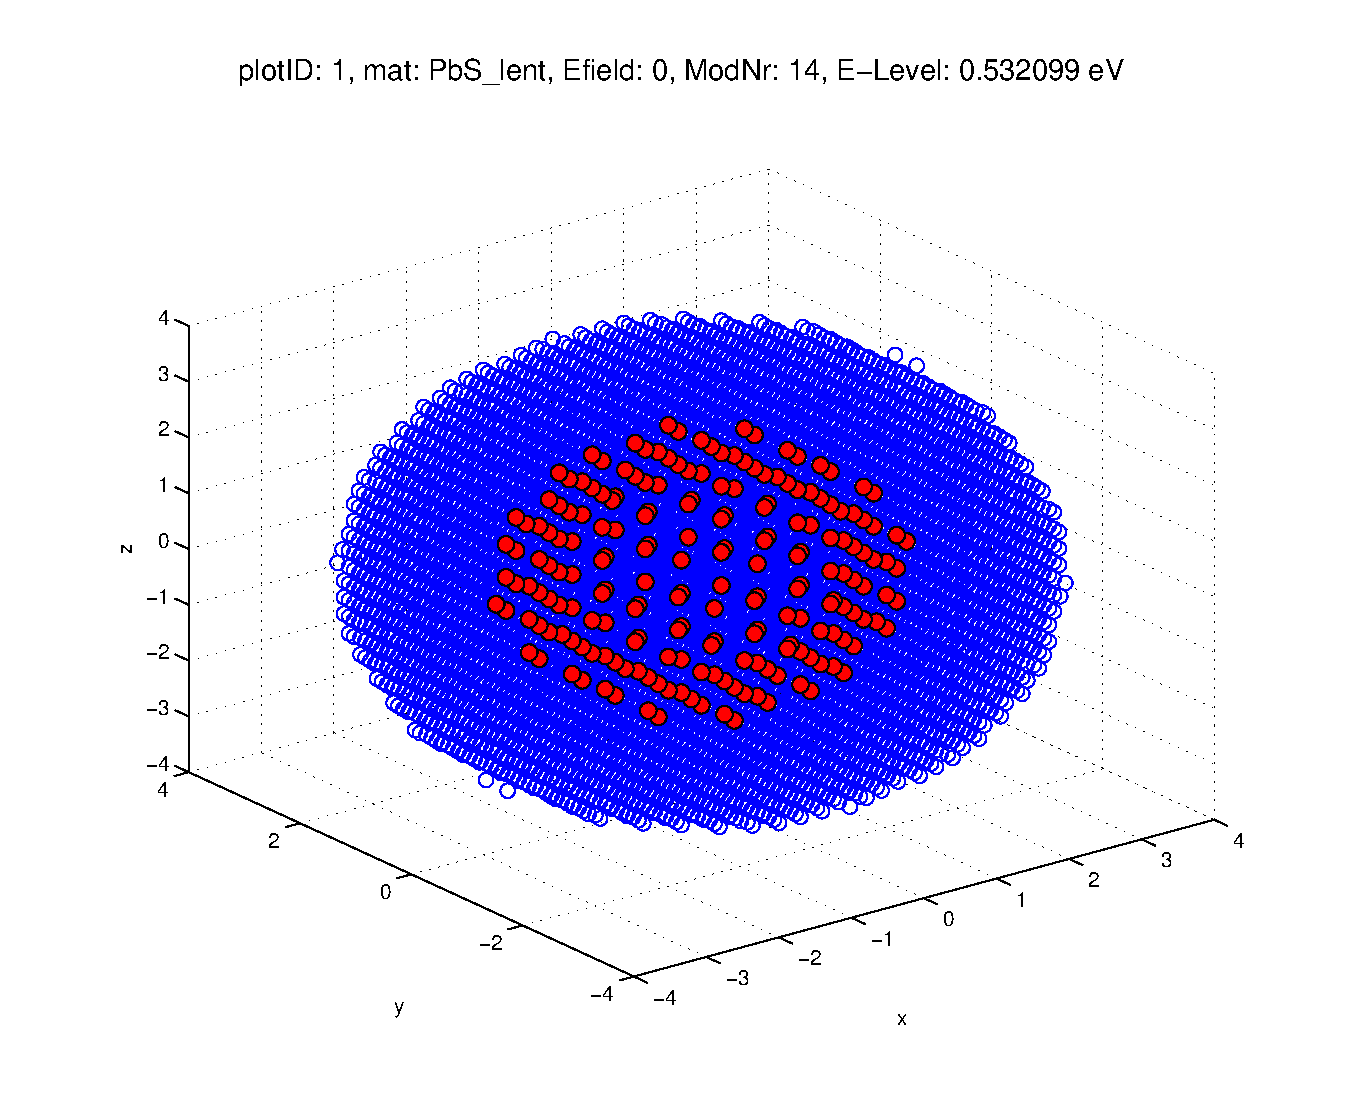
\includegraphics[width=150px]{Fig/Plots/r4CBmod14}
		\caption{}
	\end{subfigure}
	\begin{subfigure}{150px}
		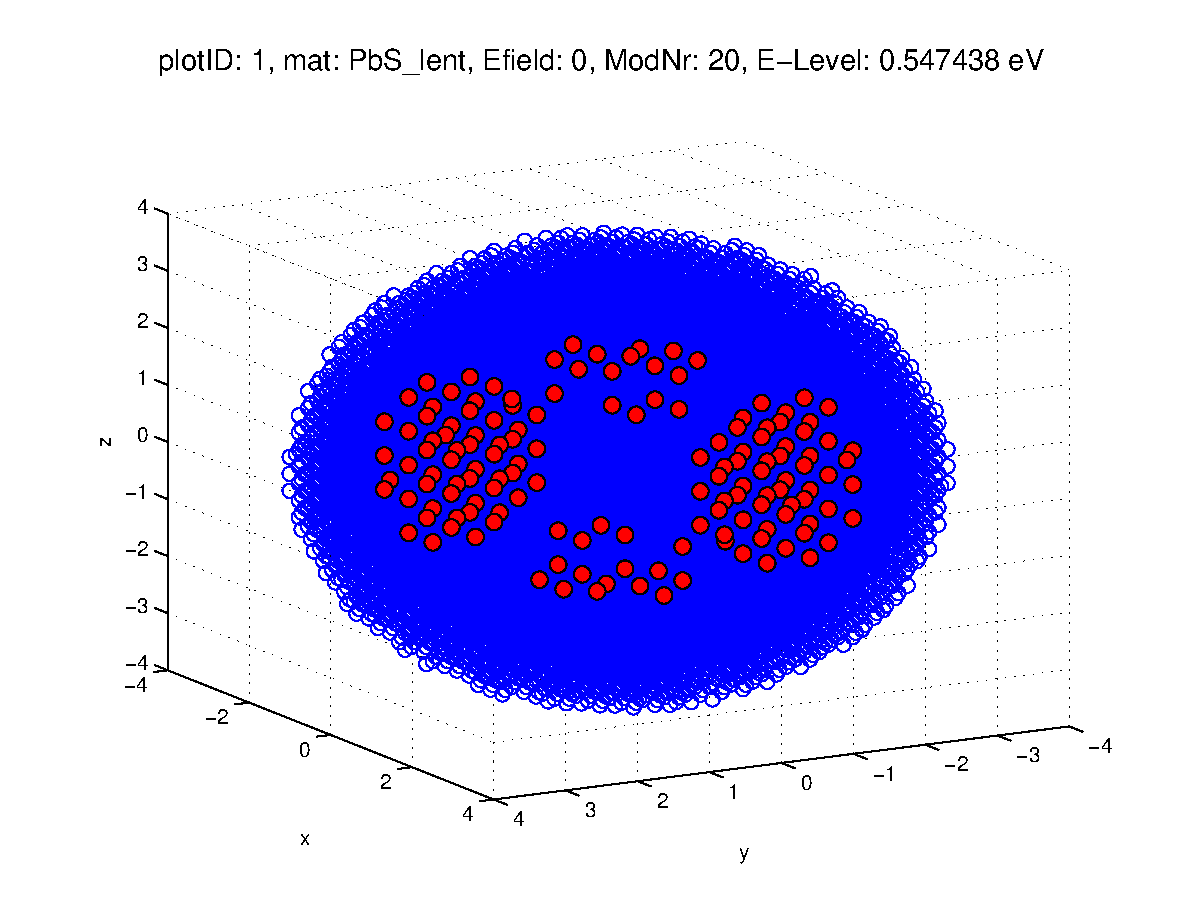
\includegraphics[width=150px]{Fig/Plots/r4CBmod20}
		\caption{}
	\end{subfigure}
	\caption{Probability density for higher energy states in an 8nm QD: barbell-shape (a), spherical shell-shape (b), crossed barbell-shape (c). In plots (b) and (c) the locations of medium high probability (yellow points) are not shown for clarity.}
	\label{fig:HigherModWaveFn}
\end{figure}
%

% TEXT
\begin{REMARK}
Although the term \textit{wave function} appears a lot in this section, the term is rather meant in the sense of \textit{probability density}, since the plots, on which the analysis is based, are more easily interpreted if they show probabilities instead of complex numbers.
\end{REMARK}

Sometimes, the wave functions of QDs are described in analogy to atomic orbitals, labeled S, P, D and so on, with subscript e or h, denoting electron-like (conduction band) states or hole-like (valence band) states respectively. We will see how well this picture corresponds to the simulation.

The 8 energy states (`modes') closest to the band edge (for conduction and valence band respectively) have wave functions with spherical symmetry, where the highest probability density is in the center (figure~\ref{fig:sphericalWaveFn}). This is in agreement with the 8 predicted $1S_{e,h}$ orbitals for PbS \cite[p.410]{Talapin}.
	
The higher energy states show wave functions with more complex shapes. For example, a 8nm QD shows the following wave function shapes: After the 8 spherical conduction band states follow 4 (degenerate) states with barbell shape, in different orientations. Then 2 states with spherical shell shape. After that, 2 states with a shape similar to two crossed barbells. Then again 2 spherical shell-like states, followed by 2 ring-shaped wave functions, and so on (figure~\ref{fig:HigherModWaveFn}). For the valence band states, the shapes are similar, although they do not occur in the same order (the same is true for QDs of different sizes).

\subsubsection{QDs smaller than 3nm}	

%FIGURES
\begin{figure}[htbp]
	\centering
	\begin{subfigure}{200px}
		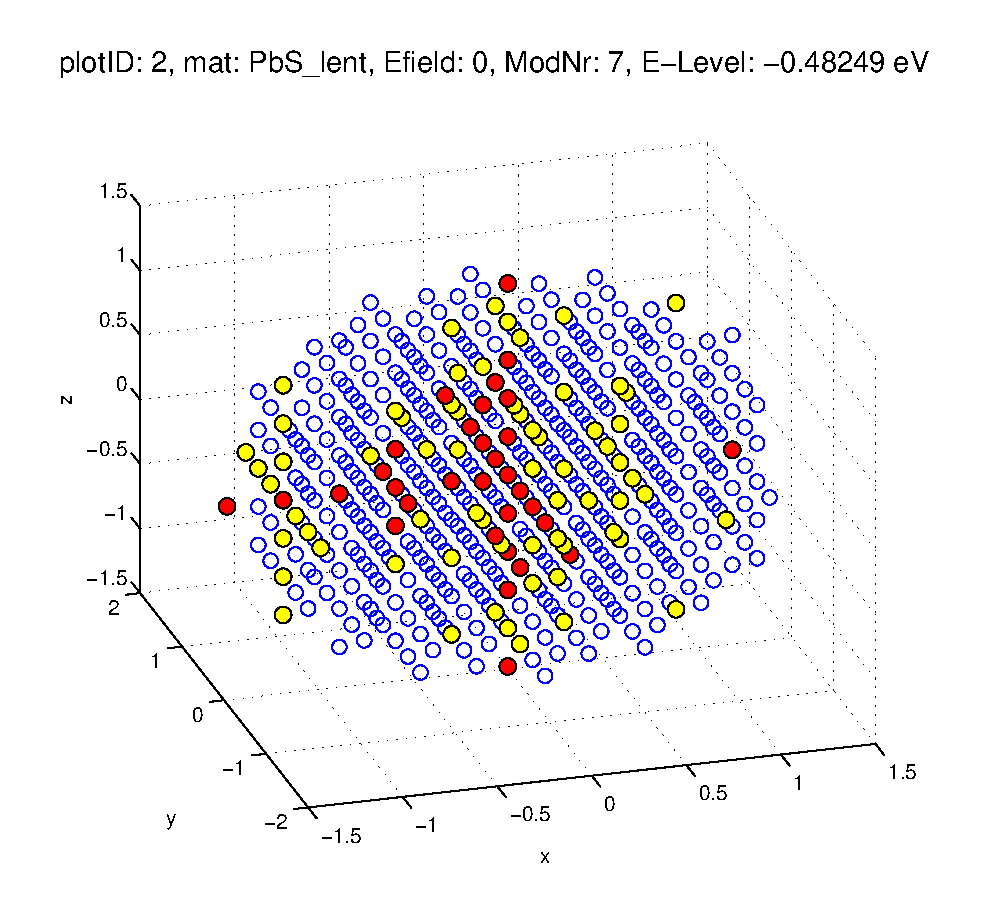
\includegraphics[width=200px]{Fig/Plots/r15VBmod7}
		\caption{3nm QD. 7th valence band state.}
	\end{subfigure}
	\begin{subfigure}{200px}
		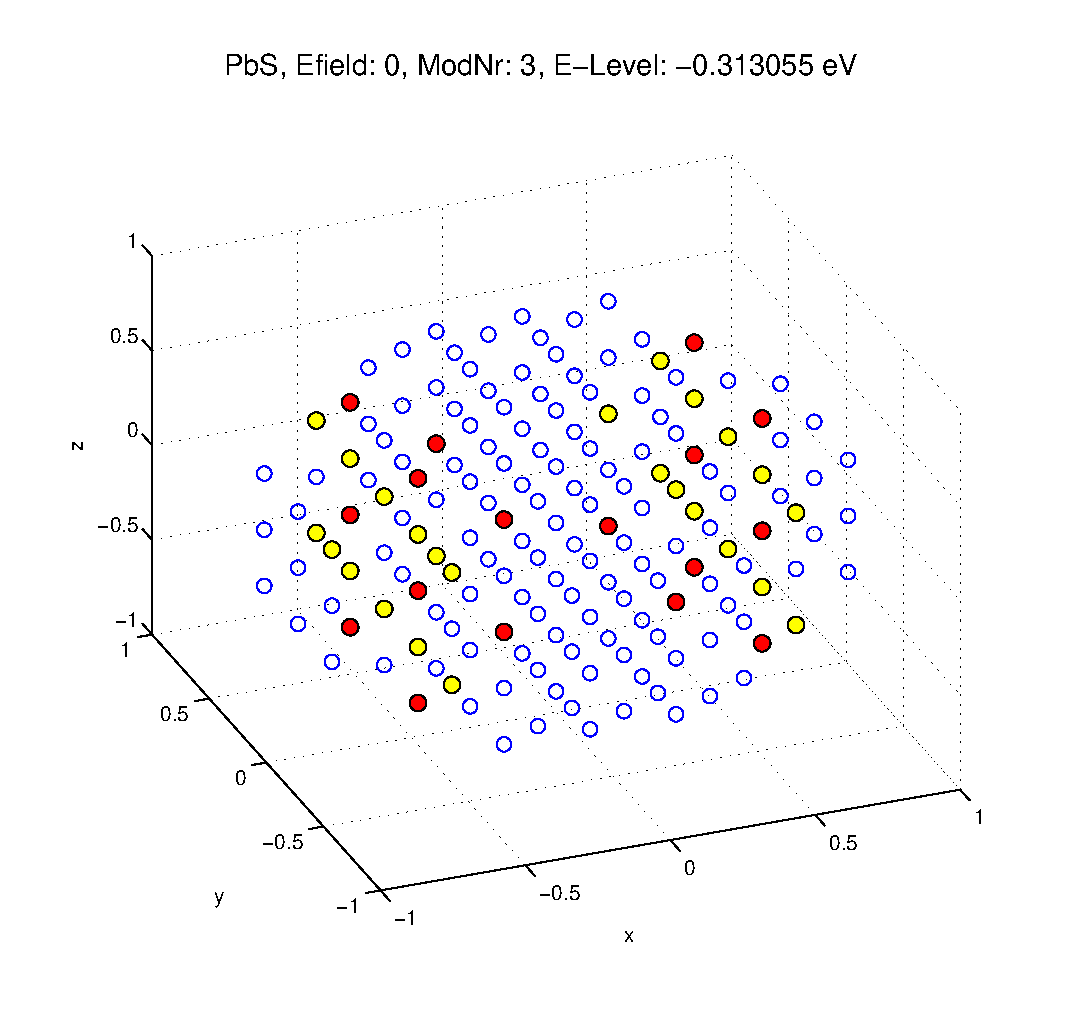
\includegraphics[width=200px]{Fig/Plots/r1VBmod3}
		\caption{2nm QD. 3rd valence band state.}
	\end{subfigure}
	\caption{Probability density for valence band states. The shape starts to deviate from the previously spherical shapes.}
	\label{fig:asymWaveFn}
\end{figure}


%TEXT
For QDs smaller than 3nm, the problem is that it is more difficult to see the shape of the wave function (too few atoms). Furthermore it is not clear how well this models a real QD, since the surface (and thus passivation of the surface) begins to have an even bigger influence.
	
For 2 and 3nm QDs, the 8 lowest conduction band states still remain more or less spherical. Whereas the valence band states start to lose spherical symmetry. For a 3nm QD, mode 7 and 8 are already slightly asymmetric (figure~\ref{fig:asymWaveFn} (a)), and for the 2nm QD, even the modes 1 to 4 are clearly not spherical, but the wave function is rather localized at two sides (figure~\ref{fig:asymWaveFn} (b)).
	
\FloatBarrier
\subsection{Influence of an electric field}

%FIGURES
\begin{figure}[htbp]
	\centering
	\begin{subfigure}{200px}
		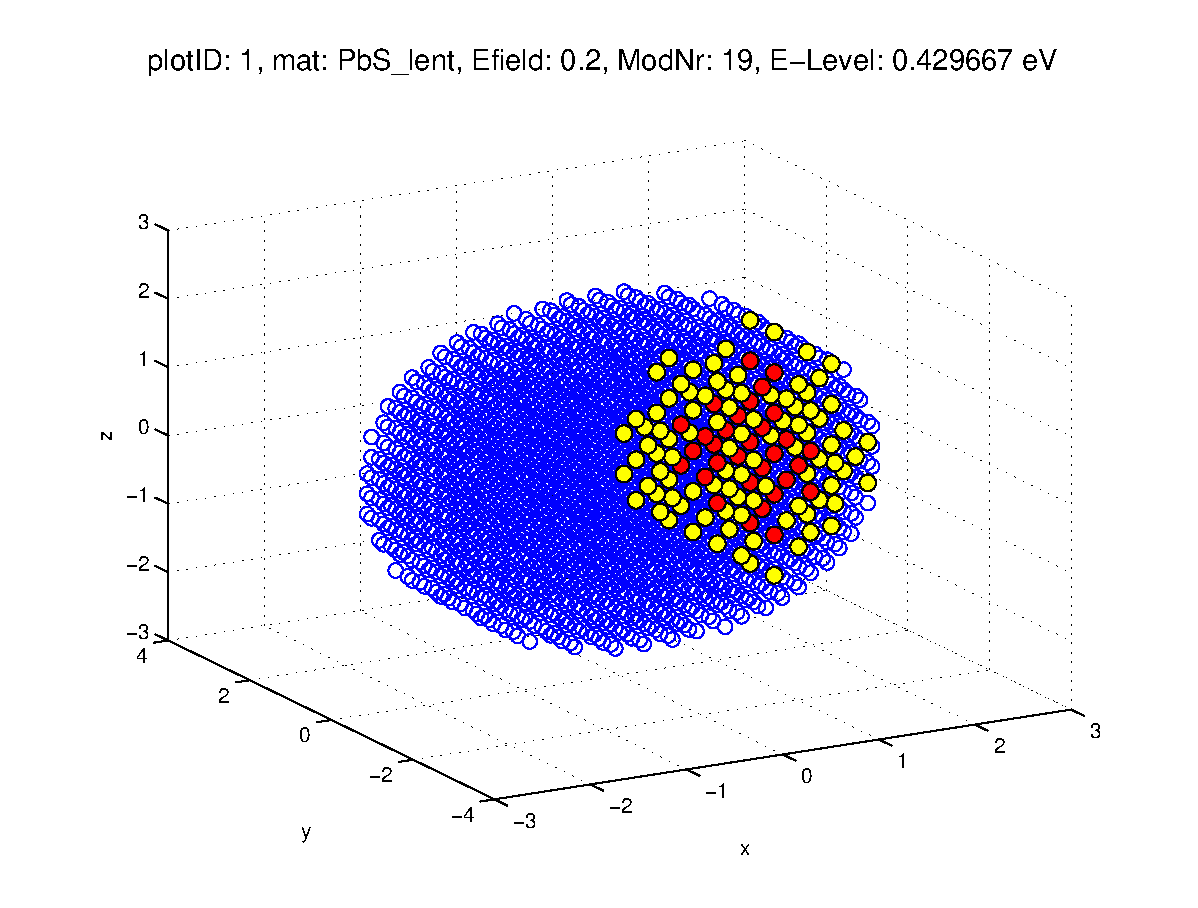
\includegraphics[width=200px]{Fig/Plots/r25v02CB}
		\caption{Conduction band state}
	\end{subfigure}
	\begin{subfigure}{200px}
		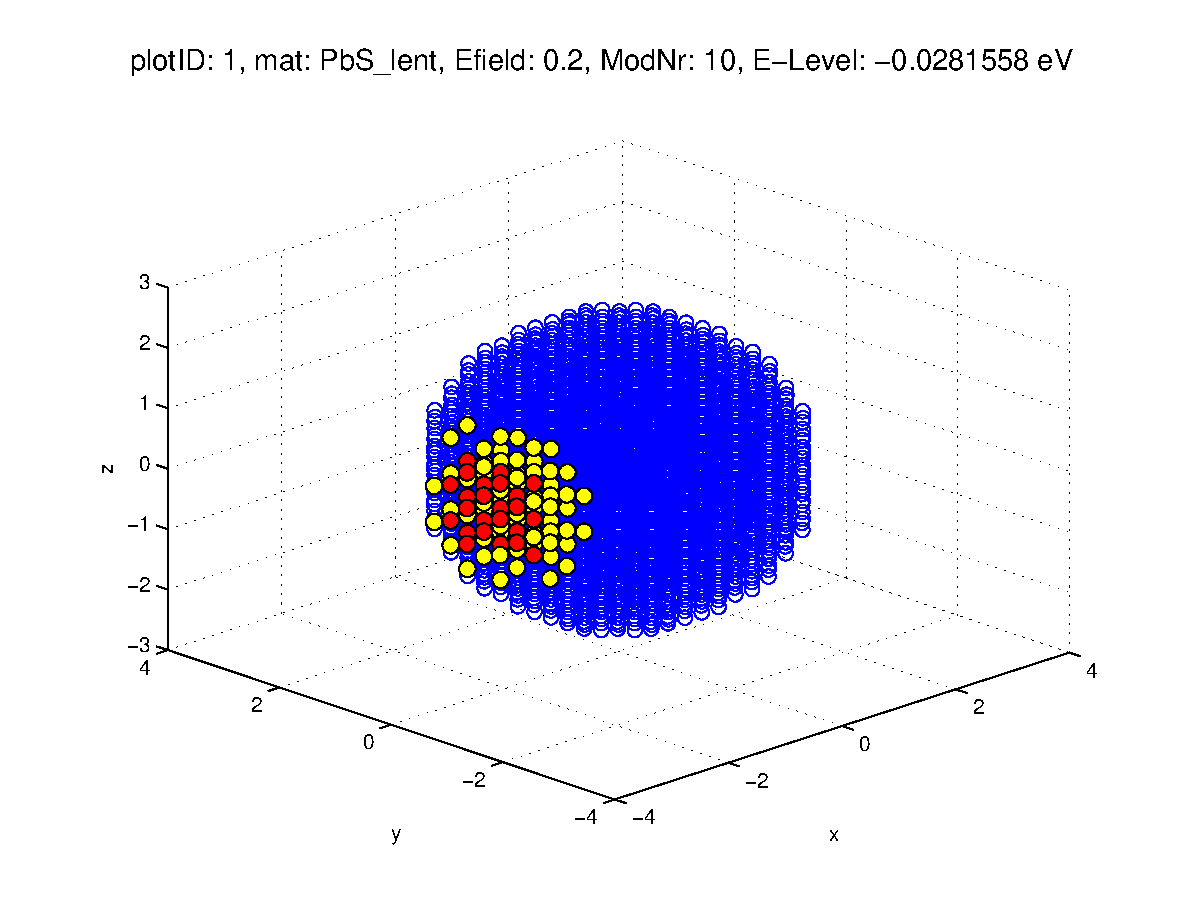
\includegraphics[width=200px]{Fig/Plots/r25v02VB}
		\caption{Valence band state}
	\end{subfigure}	
	\caption{Probability densities for a 5nm QD in an electric field of 0.2V/nm.}
	\label{fig:EfieldWaveFn}
\end{figure}
%
\begin{figure}[htbp]
	\centering
	\begin{subfigure}{150px}
		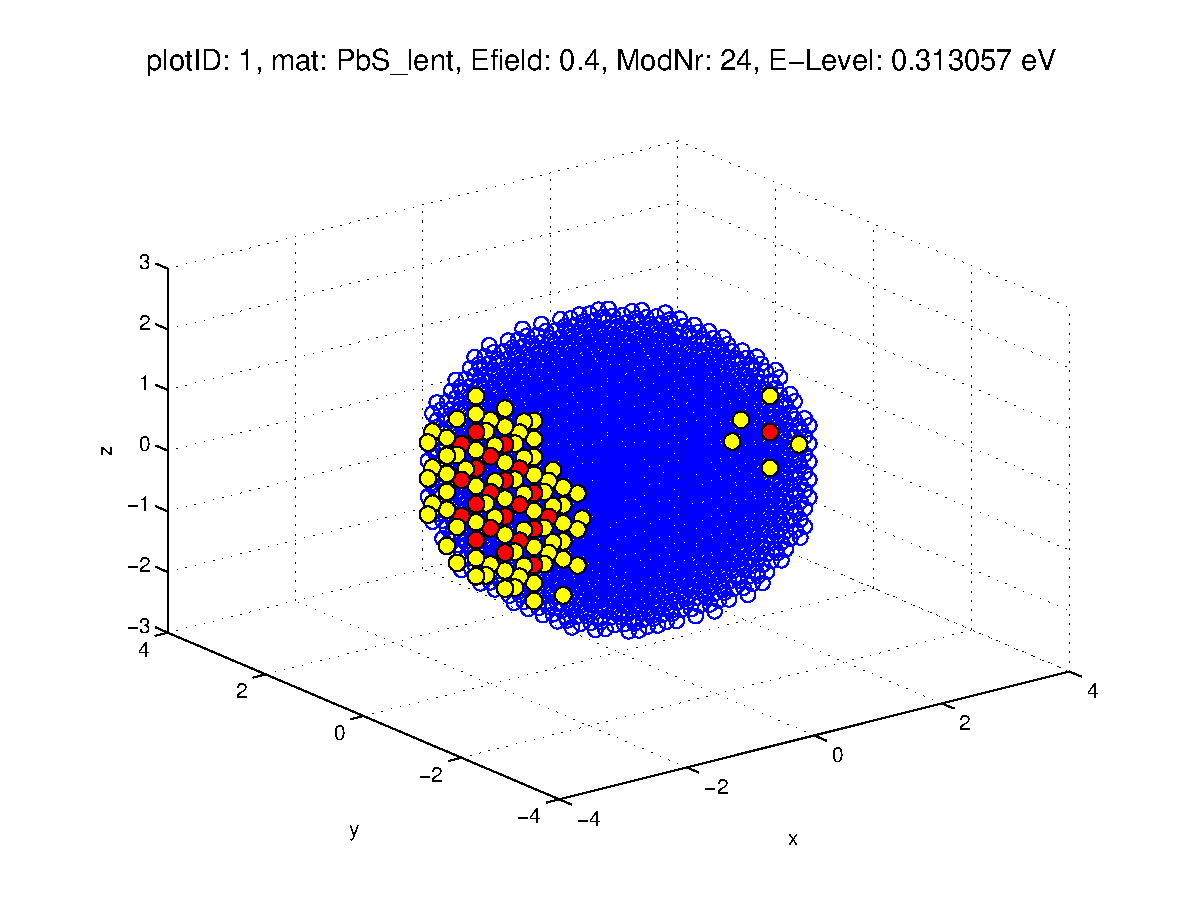
\includegraphics[width=150px]{Fig/Plots/r25v04Mod24}
		\caption{Eigenstate at 0.313057eV}
	\end{subfigure}
	\begin{subfigure}{150px}
		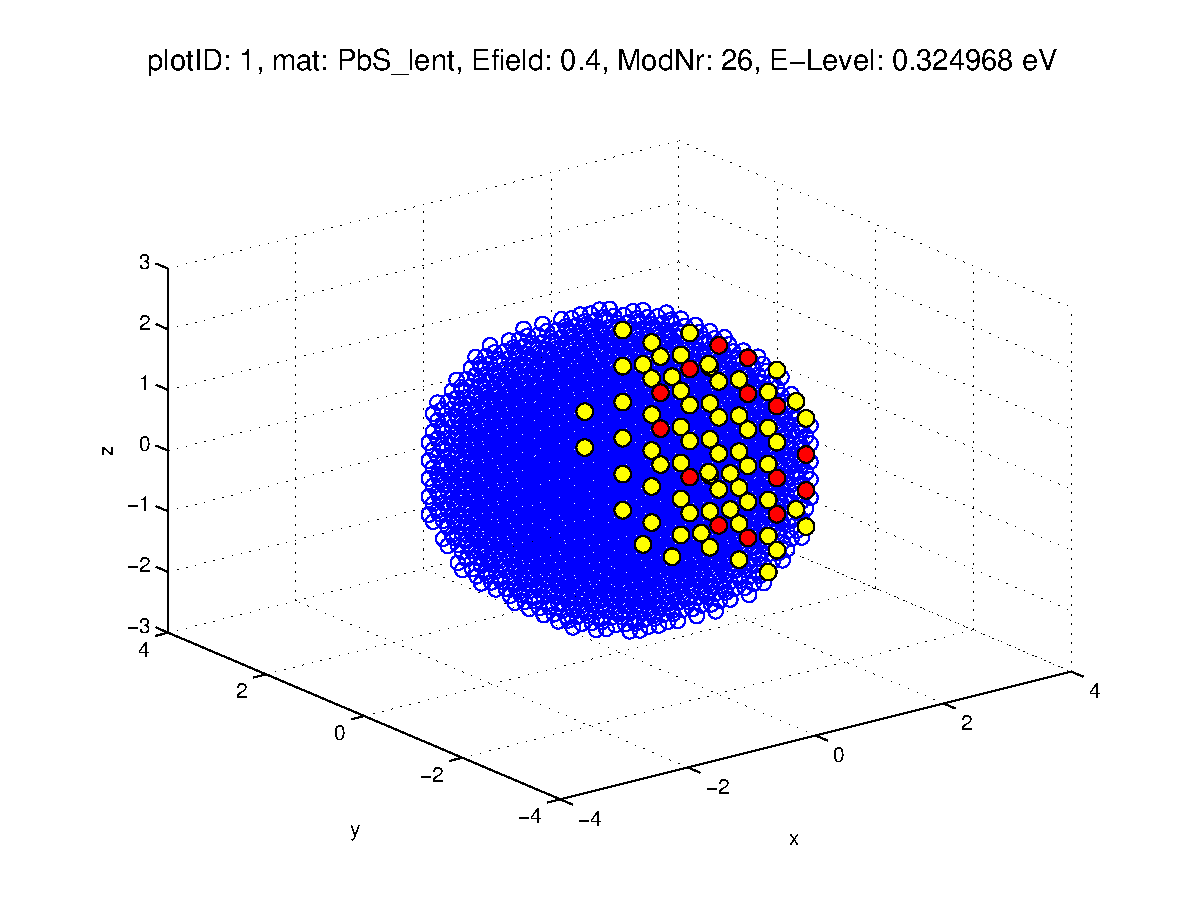
\includegraphics[width=150px]{Fig/Plots/r25v04Mod26}
		\caption{Eigenstate at 0.324968eV}
	\end{subfigure}
	\begin{subfigure}{150px}
		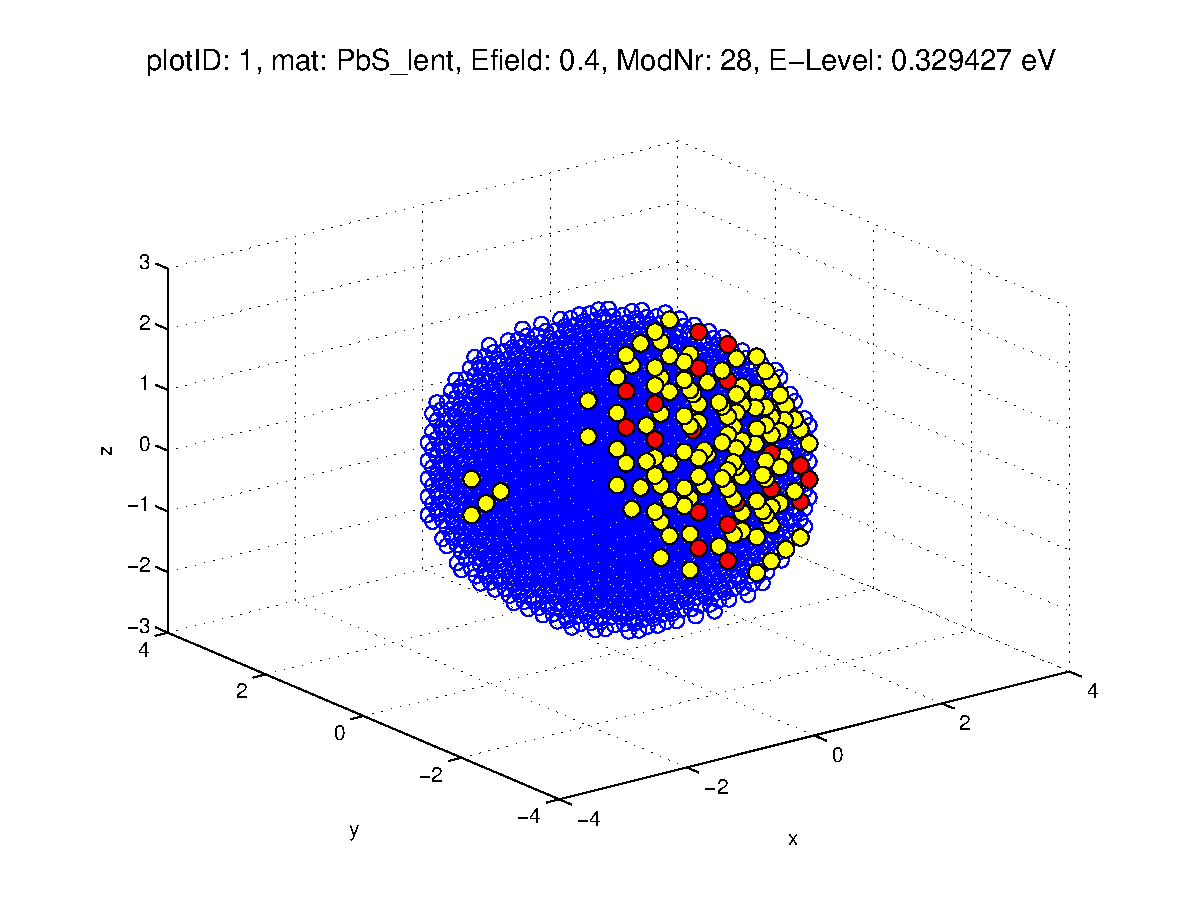
\includegraphics[width=150px]{Fig/Plots/r25v04Mod28}
		\caption{Eigenstate at  0.329427eV}
	\end{subfigure}
	\begin{subfigure}{150px}
		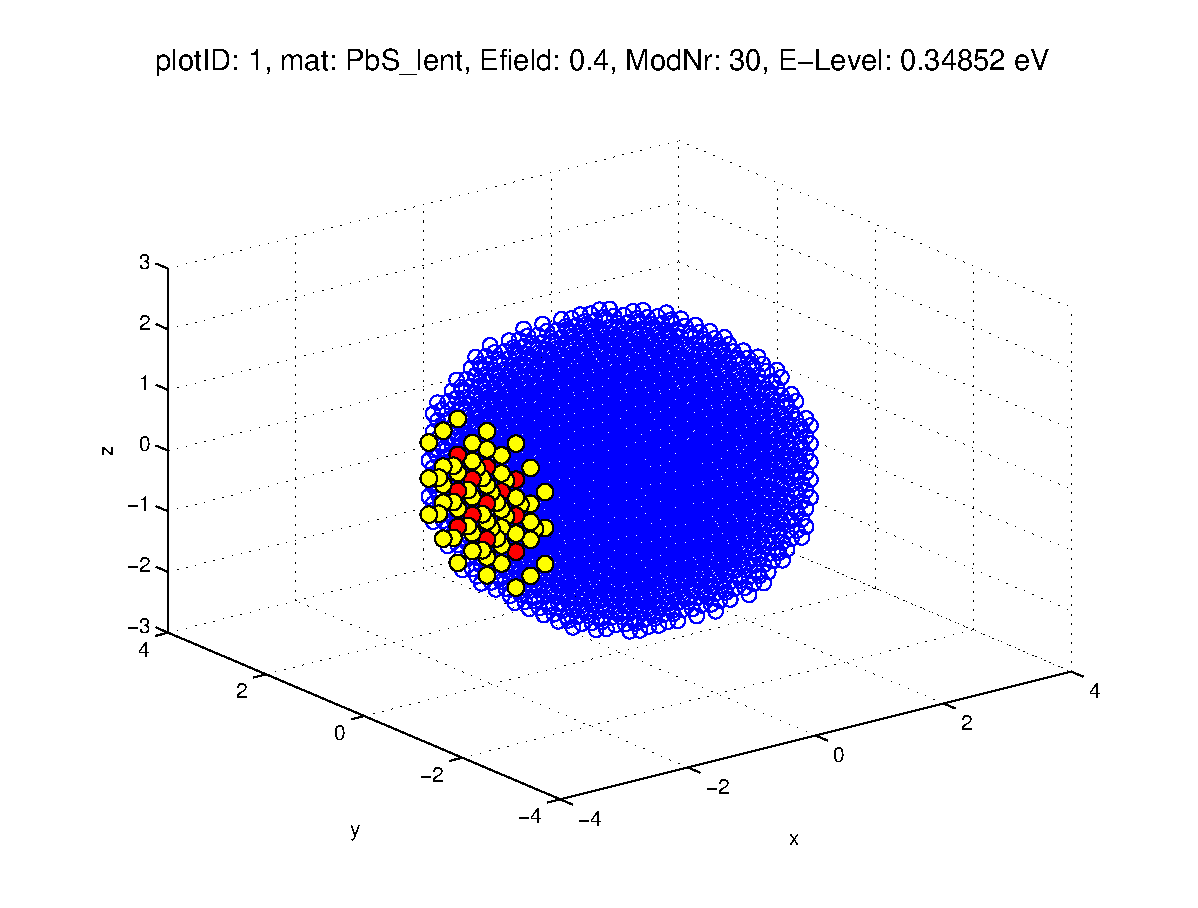
\includegraphics[width=150px]{Fig/Plots/r25v04Mod30}
		\caption{Eigenstate at 0.34852eV}
	\end{subfigure}
	\begin{subfigure}{150px}
		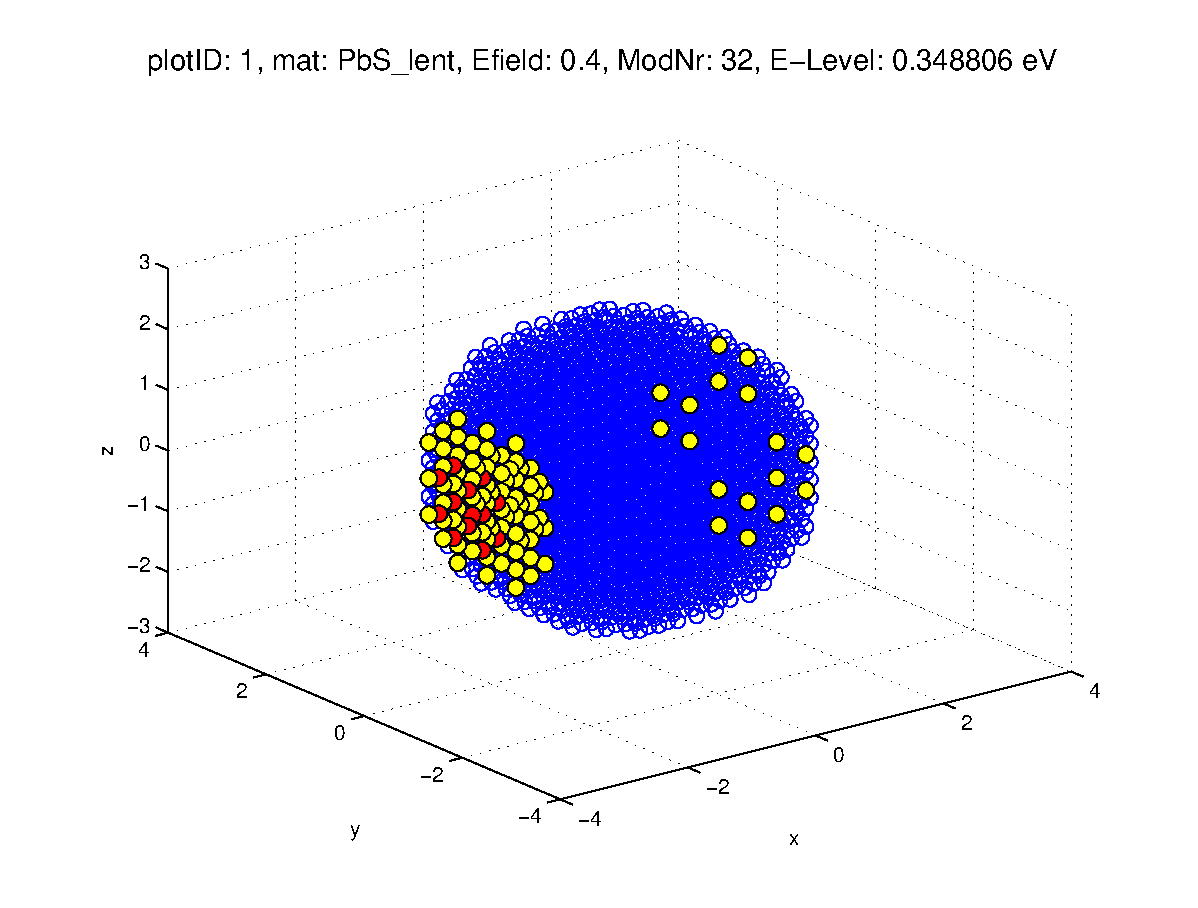
\includegraphics[width=150px]{Fig/Plots/r25v04Mod32}
		\caption{Eigenstate at 0.348806eV}
	\end{subfigure}
	\begin{subfigure}{150px}
		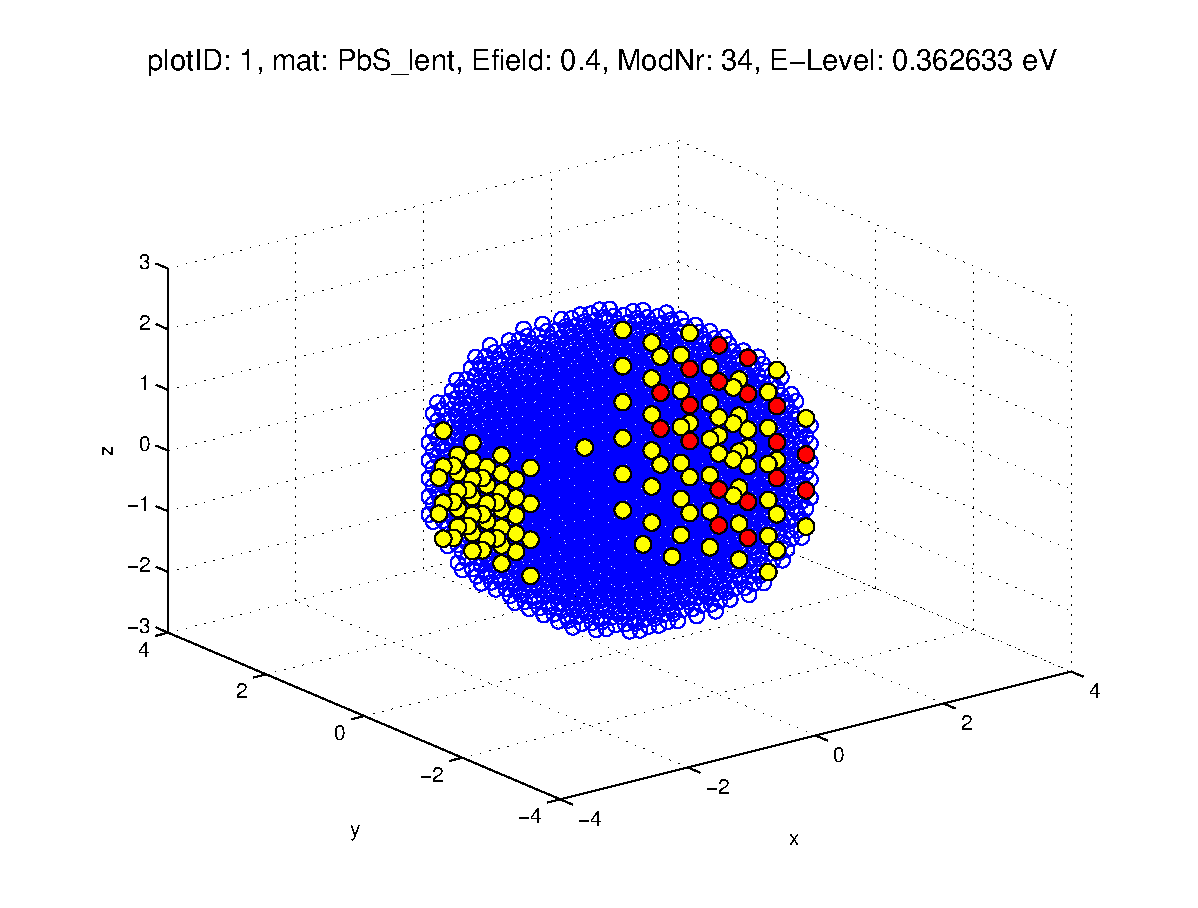
\includegraphics[width=150px]{Fig/Plots/r25v04Mod34}
		\caption{Eigenstate at 0.362633eV}
	\end{subfigure}
	\caption{Probability densities in the presence of a high electric field (0.4V/nm). Increasing energy from (a) to (f). Hole-like states (a),(d),(e) become mixed with electron-like states (b),(c),(f).}
	\label{fig:HighEfieldWaveFn}
\end{figure}


%TEXT
The presence of an electric field results in a shift of the wave function, i.e.~the maximum of the probability density is not in the center anymore and the spherical symmetry of the 8 first states is broken (for conduction and valence band respectively). Furthermore, one can see that the valence band states really behave differently than conduction band states: The wave function is shifted in the opposite direction (figure~\ref{fig:EfieldWaveFn}). This confirms that the valence band states are hole-like, similar to bulk semiconductor band theory. 
	
For larger electric fields the band gap gets smaller, until it finally disappears, i.e. conduction and valence band states are not separated anymore. For example, for a 5nm  QD, the band gap disappears for electric fields larger than 0.35 V/nm (figure~\ref{fig:EvsVolt}). The states close to the (former) band gap cannot be separated in conduction and valence band: as energy increases, some hole-like states are followed by electron-like (i.e.~conduction band-like) states, which in turn are followed by hole-like states and later again electron-like states (figure~\ref{fig:HighEfieldWaveFn}).
	
Additionally, with higher electric fields, the wave functions seem not only to be shifted, but change shape: Some now look more like asymmetric barbells or even stranger, ring-like shapes (figure~\ref{fig:HighEfieldWaveFn} (a) and (f)).

\FloatBarrier

\section{Conclusions}

We have seen that larger PbS QDs have eightfold degenerate energy states at the band edges, whose wave functions have spherical symmetry. Higher energy states show more complex wave functions. For QDs smaller than 3nm, the eightfold degeneracy is lost more and more, as well as the spherical symmetry of these wave functions. However, it is questionable how close to reality the simulations of very small structures below 2nm are.
Under the influence of an electric field, the wave functions shift, according to their being hole- or electron-like, in opposite directions.

Furthermore we noticed, that the band gap is depending on size and the applied voltage. Increasing the voltage, energy levels get closer and
cause a narrowing of the band gap.
	\chapter{Simulations with \software}

	\software was programmed to simulate spherical nanocrystals and to visualize the results of the simulations.
	Though we focused on spherical structures, the code is hold abstract and slim to make extending to other
	structures, such as nanowires, fairly easy.
	The main aim of \software is to offer \omen users a toolbox, which includes the following 3 main tasks:
	\begin{enumerate}
		\itemsep 0pt
		\item Automatization of the \omen simulation process \\
					When it comes to simulating quantum dots with different parameters users do not want to spend a lot
					of time on writing command files for OMEN by themselves and start each OMEN task via the shell, but 
					rather enter the main parameters into a \gls{GUI} and let \software do the rest (see section \ref{sec:RunSim}).
					This makes overnight simulations for large parameter sets possible.
		\item Overview of all simulations done in the past	\\
					All information respectively parameters of past simulations can be displayed in a \gls{GUI}. Exporting selected
					simulations and visualizing them is possible as well (see section \ref{sec:guiDB})
		\item Visualization of simulation data	\\
					All different kinds of plots are available within the toolbox, such as visualizing band gaps, wave functions or
					quantum dot structures (see section \ref{sec:Visualization}).
	\end{enumerate}

	\section{Installing the Software}
		*********************** \\
		****** TO DO !!! ****** \\
		*********************** \\
	
	\section{Using \software}
		\subsection{Running a simulation} \label{sec:RunSim}
			Type gui\_simulate \index{gui\_simulate} in the \matlab command window and hit enter. The window as in figure \ref{fig:gui_simulate} will open.
			\begin{figure}[htbp]
				\centering
				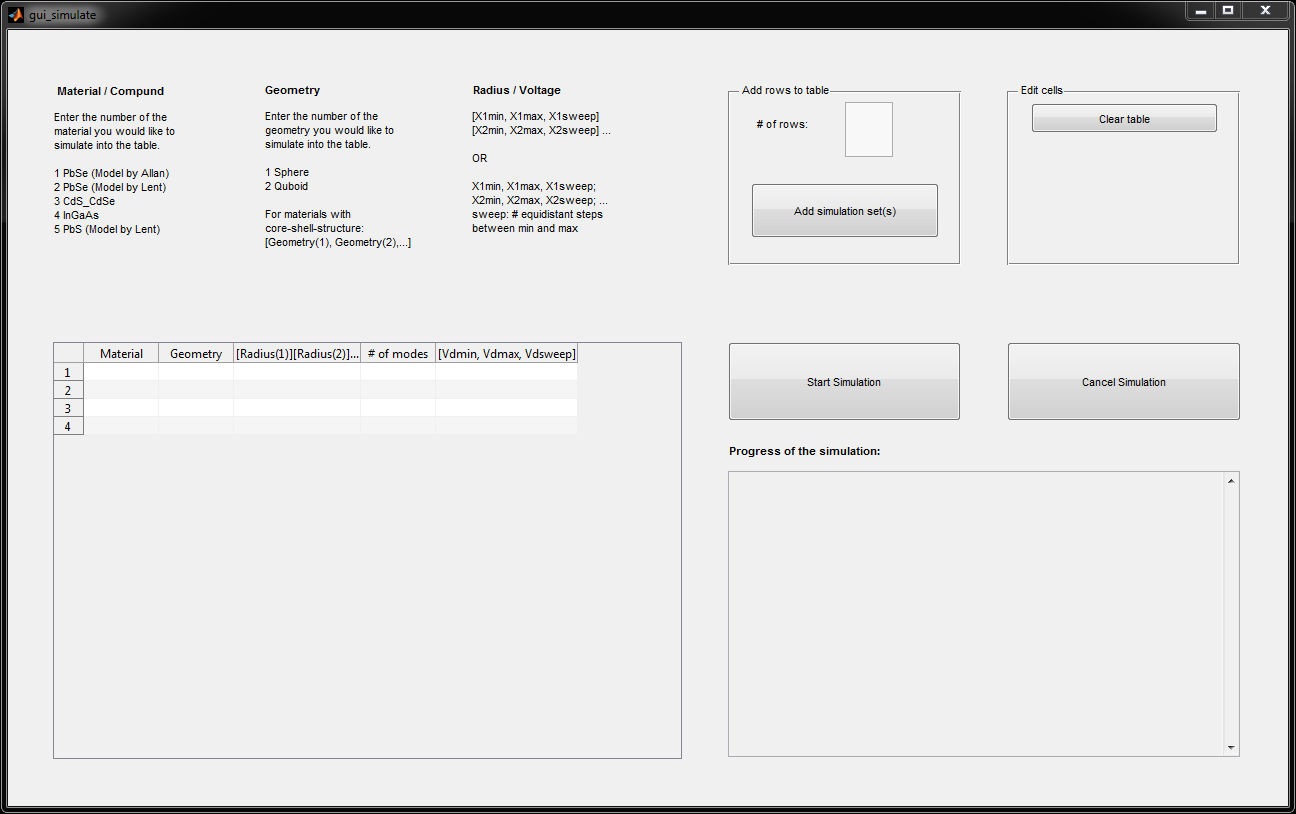
\includegraphics[width=0.6\textwidth]{Fig/Scrn_gui_simulate.png}
				\caption{The gui\_simualte window}
				\label{fig:gui_simulate}
			\end{figure}
			A simulation set is defined as one row of the table, i.e one material with all kinds of sweeps. You can add more simulation sets
			by using the {\it Add rows to the table} panel.
			It is possible to copy and paste single cells of the table using the appropriate short cuts of your \matlab default keyboard setup
			(\verb|CTRL+C & CTRL+V| Windows setting, \verb|ALT+W & CTRL+Y| Emacs setting).
			The columns are filled as follows:
			\begin{enumerate}
				\item Material		\\
							Enter the number for the material you would like to simulate, according to the {\it Material / Compound} list.
				\item Geometry		\\
							Enter the number of the geometry given in the {\it Geometry} list. Very important in the case of materials with
							shells is, that you have to enter the geometry type of the core and the shell. The geometry types are separated	
							with a comma.
							\begin{EXAMPLE}
								For a spherical CdS-CdSe quantum dot the cell would look like this: 1, 1
							\end{EXAMPLE}
				\item Radius			\\
							The radius has to be entered in a specific way. The syntax is: \\
							\verb|[Rmin(1), Rmax(1), Rsweep(1)][Rmin(2), Rmax(2), Rsweep(2)]...| \\
							\newline
							\begin{tabular}{@{}ll}
								\verb|Rmin(i)|		& smallest radius of the i\textsuperscript{th} material to be simulated				\\
								\verb|Rmax(i)|		& largest radius of the i\textsuperscript{th} material to be simulated				\\
								\verb|Rsweep(i)|	& number of equidistant points between \verb|Rmin(i)| \& \verb|Rmax(i)|		\\
							\end{tabular}
							
							\begin{EXAMPLE}
								Simulation a single spherical PbS quantum dot with radius 3.5 nm you would enter: [3.5,3.5,1]
							\end{EXAMPLE}
							
							\begin{EXAMPLE}
								For a spherical CdS-CdSe quantum dot the cell would look like this: [1,4,4][5,6,2]
								Looking at the radius parameters, \software will do all the permutations and generate therefore 8 quantum dots: \\
								\newline
								\begin{tabular}{@{}lcccccccc}
									Quantum dot					&	1	&	2	&	3	&	4 &	5	&	6	& 7	&	8	\\
									Core radius	in nm		&	1	& 1 & 2 & 2 & 3	& 3 & 4 & 4	\\
									Shell radius in nm	& 5	& 6 & 5 & 6 & 5 & 6 & 5 & 6	\\
								\end{tabular}
							\end{EXAMPLE}
				\item \# of modes	\\
							Enter a number of modes you would like to calculate.
				\item Voltage			\\
							The Voltage sweep is entered in the same way as the radius. You find more information under the following remark.
			\end{enumerate}
			
			\begin{REMARK}[Vectors \& Matrices] \index{Vector}
				As the \matlab \gls{GUI}s do not accept vectors or matrices as it is known from the command window, the parameters
				have to be entered as a string and are converted to matrices later on.
				
				There are different ways how to enter the parameters. Use the one, that is the most clear for you.
				\begin{verbatim}
               a,b,c,...,d                 or
              [a,b,c,...,d]                becomes a double vector

              V = [ a b c ... d]


              [a,b,c][d,e,f]...[g,h,j]     or
               a,b,c; d,e,f;...;g,h,j      or
              [a,b,c; d,e,f;...;g,h,j]     becomes a double matrix

              M = [ a b c
                    d e f
                    . . .
                    g h j ]

              where a,b,...,j are doubles as strings.
   			\end{verbatim}
   			These input styles can be applied to column {\it Geometry}, {\it Radius} and {\it Voltage}.	\\
   			You can use as many spaces as you want in between. The first and the last brace are not necessary if only a vector is entered or if
   			rows are separated by semicolons.
			\end{REMARK}
			
			After entering all the necessary parameters proceed by clicking \verb|Start Simulation|. The {\it Progress of the simulation} panel will
			keep you informed about the warnings, wrong entered parameters and the current status of the simulation.



		\subsection{Display simulation information} \label{sec:guiDB}
			There are two ways of displaying simulation information, either you can see the whole database \index{Database} (all simulations
			that are stored in the Simulations folder) or only specific data, for example only PbS simulation data.
			
			\begin{REMARK}
				\software uses objects (called {\it qdotObj}) to store all important data of simulations such as the simulation parameters, date of simulation etc.
				(futher information section \ref{sec:SoftwareStructure}). All operations are done using these objects. If you would like to display only
				certain simulation data, you would need an {\it qdotObj} array. How to create such an array please read section \ref{sec:addTools}.
			\end{REMARK}
			
			Displaying the whole database can be done by typing \verb|gui_db| \index{gui\_db} into the \matlab command window. A window as in figure \ref{fig:gui_database} will appear
			showing all parameters and technical information of each simulation. Please note, that according to the size of the database, it might take some seconds
			to load all data.
			If you only want to display a set of simulation data, you can also call \verb|gui_db(qdotObj_ARRAY)|, where \verb|qdotObj_ARRAY| is an array of qdotQbj objects.
			
			\begin{figure}[htbp]
				\centering
				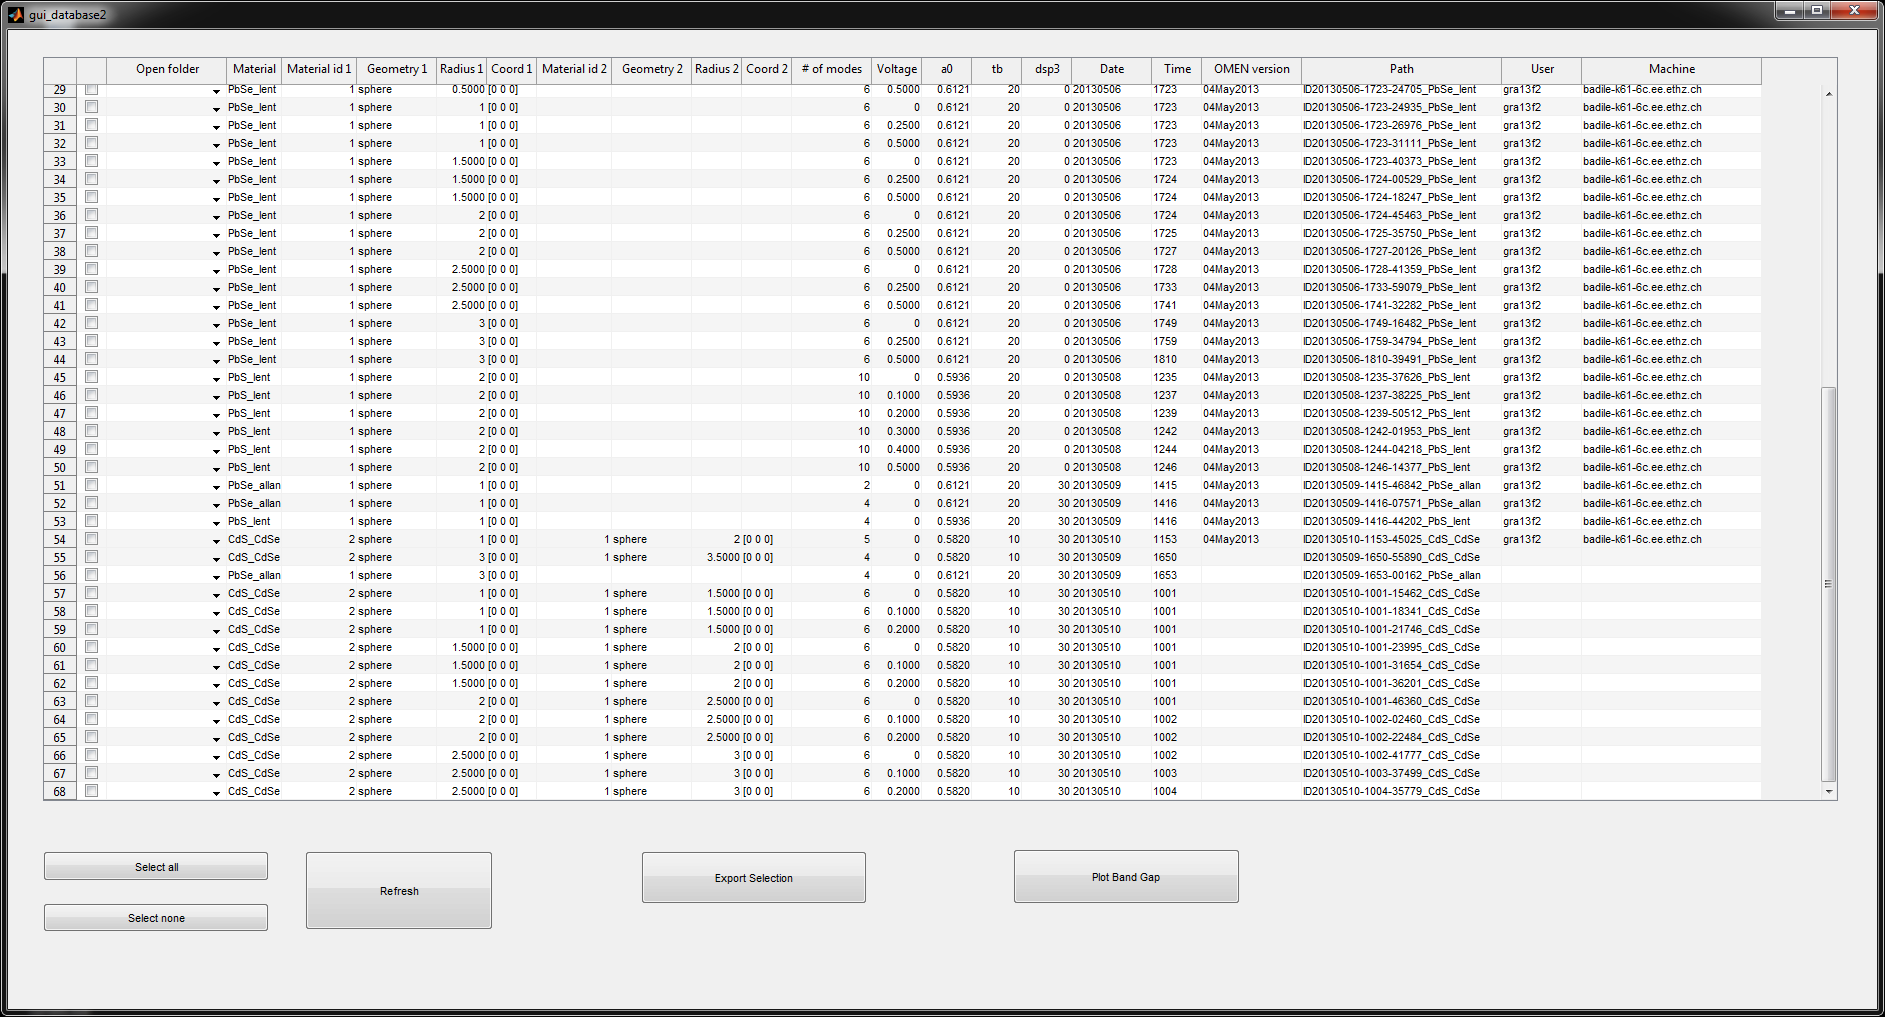
\includegraphics[width=\textwidth]{Fig/Scrn_gui_database.png}
				\caption{The gui\_database window}
				\label{fig:gui_database}
			\end{figure}
			
			Within the \gls{GUI} you can sort the simulations with the column header, select simulations and let plot them, open the directory of a simulation or 
			even export a selection, which is available as an qdotObj array in the main workspace entitled {\it ExportedDB}.


		\subsection{Visualization} \label{sec:Visualization}
			As explained in the previous section, simulation data can be visualized \index{Visualization} through the {\it gui\_database} window, but also manually.
			In this section the plotting \index{Plotting} functions are explained.
			
			\begin{lstlisting}
				plotBandGap(DB)
			\end{lstlisting}
		
		
		\subsection{Additional tools} \label{sec:addTools}
			
	
	\section{Maintaining \software}
		\subsection{General Structure} \label{sec:SoftwareStructure}
		
			\begin{figure}[htbp]
				\begin{minipage}[b]{0.59\textwidth}
				% Creates a directory structure figure
				\dirtree{%
				.1 /root.
					.2 MATLAB.
						.3 Classes.
						.3 Functions.
						.3 GUI.
						.3 System.
					.2 OMEN executable.
					.2 Simulations.
						.3 ID*.
						.3 \vdots.
						.3 log.
				}
				\caption{The \software structure by default}
				\label{dir:ToolboxTree}
			\end{minipage}
			\hfill
			\begin{minipage}[b]{0.39\textwidth}
			\dirtree{%
			.1 ID*.
				.2 CB\_E\_0\_0.dat.
				.2 CB\_V\_0\_0.dat.
				.2 H\_0.dat.
				.2 Layer\_Matrix.dat.
				.2 qdot\_cmd.
				.2 qdotObj.mat.
				.2 simlog\_{\it yyyymmdd\_hhmm\_ssfff}.
				.2 VB\_E\_0\_0.dat.
				.2 VB\_E\_0\_0.dat.
			}
			\caption{Structure of a simulation set}
			\label{dir:SimSetTree}
			\end{minipage}
			\end{figure}
			
			\begin{lstlisting}[frame=single]
				IDyyyymmdd-hhmm-ssfff_MATNAME
			\end{lstlisting}
				
			\begin{lstlisting}[frame=single]
			struct global config {
				config.root        = '';
				config.system      = '';
				config.log         = '';
				config.user        = '';
				config.machine     = '';
				config.OMEN        = '';
				config.simulations = '';
				config.vOMEN       = '';
				config.cancelSim   = '';
			}
			\end{lstlisting}
			
%	\subsection{Installing and setting up \software}
%		\subsection{\acl{GUI}}
%			\subsubsection{Starting a new Simulation}
%			
%			\subsubsection{}
%		
%		\subsection{OMEN Procedures}
%		
%		\subsection{Visualization}
	%\documentclass[10pt,a4paper]{book}

\usepackage[left=2.5cm, right=2cm, top=2cm, bottom=2cm]{geometry}
\usepackage[latin1]{inputenc}
\usepackage[T1]{fontenc}

\usepackage{graphicx}
\usepackage{color}
\usepackage{tikz}
	\usetikzlibrary{shapes,arrows}
\usepackage{dirtree}

\usepackage{amsmath}
\usepackage{amsfonts}
\usepackage{amssymb}
\usepackage{listings}
\usepackage{blindtext}

\usepackage{color}

\definecolor{mygreen}{rgb}{0,0.6,0}
\definecolor{mygray}{rgb}{0.5,0.5,0.5}
\definecolor{mymauve}{rgb}{0.58,0,0.82}

\lstset{ %
  backgroundcolor=\color{white},   % choose the background color; you must add \usepackage{color} or \usepackage{xcolor}
  %basicstyle=\footnotesize,        % the size of the fonts that are used for the code
  basicstyle=\ttfamily,%\footnotesize,
  breakatwhitespace=false,         % sets if automatic breaks should only happen at whitespace
  breaklines=true,                 % sets automatic line breaking
  captionpos=b,                    % sets the caption-position to bottom
  columns=fixed,
  commentstyle=\color{mygreen},    % comment style
  deletekeywords={...},            % if you want to delete keywords from the given language
  escapeinside={\%*}{*)},          % if you want to add LaTeX within your code
  extendedchars=true,              % lets you use non-ASCII characters; for 8-bits encodings only, does not work with UTF-8
  %frame=single,                    % adds a frame around the code
  keepspaces=true,                 % keeps spaces in text, useful for keeping indentation of code (possibly needs columns=flexible)
  keywordstyle=\color{blue},       % keyword style
  language=Matlab,                 % the language of the code
  morekeywords={*,...},            % if you want to add more keywords to the set
  %numbers=left,                    % where to put the line-numbers; possible values are (none, left, right)
  numbers=none,
  %numbersep=5pt,                   % how far the line-numbers are from the code
  numberstyle=\tiny\color{mygray}, % the style that is used for the line-numbers
  rulecolor=\color{black},         % if not set, the frame-color may be changed on line-breaks within not-black text (e.g. comments (green here))
  showspaces=false,                % show spaces everywhere adding particular underscores; it overrides 'showstringspaces'
  showstringspaces=false,          % underline spaces within strings only
  showtabs=false,                  % show tabs within strings adding particular underscores
  %stepnumber=2,                    % the step between two line-numbers. If it's 1, each line will be numbered
  stringstyle=\color{mymauve},     % string literal style
  tabsize=3,                       % sets default tabsize to 2 spaces
  title=\lstname                   % show the filename of files included with \lstinputlisting; also try caption instead of title
}


\begin{document}
\tikzstyle{decision} = [diamond, draw, fill={blue!25!black}, text=white,
    text width=2cm, text badly centered, node distance=3cm, inner sep=0pt]
\tikzstyle{block} = [rectangle, draw, fill=blue, text=white,
    minimum width=4cm, height=2cm]
\tikzstyle{box} = [rectangle, draw, text=black,
    width=12cm, height=18cm, node distance=8cm]
\tikzstyle{line} = [draw, -latex']
\tikzstyle{cloud} = [draw, ellipse,fill=red!20, node distance=3cm,
    minimum height=2cm]


\begin{figure}
	\centering
	\begin{tikzpicture}
		\node [box] (gui) {
		\begin{tikzpicture}[node distance = 1.5cm, auto]
    	\node [block] (guiSimulate) {function gui\_simulate};
    	\node [block, below of=guiSimulate] (simProcedure) {function simProcedure()};
			\node [block, below of=simProcedure] (writeQdot) {writeQdot()};
			\end{tikzpicture}
		};
		\node [box, below of=gui] (boxsimAll) {
			simAll                                                              \hfill \newline \\
		\begin{tikzpicture}[node distance = 1.5cm, auto]
			\node [block] (sweep) {function sweep};
			\node [block, below of=sweep] (writeCmd) {write Cmd file};
			\node [block, below of=writeCmd] (OMEN) {OMEN};
			\node [block, below of=OMEN] (logfile) {log file};
			\node [block, below of=logfile] (globallog) {global log file};
			\node [cloud, right of=OMEN] (counter) {for length of QDOA};
	    \path [line] (sweep) -- node[midway,right] {QDOA} (writeCmd);
	    \path [line] (writeCmd) -- (OMEN);
	    \path [line] (OMEN) -- (logfile);
	    \path [line] (logfile) -- (globallog);
	    \path [line] (logfile) -| (counter);
	    \path [line] (counter) |- (writeCmd);
		\end{tikzpicture}
		};
		\node [cloud, right of=gui] (setcounter) {for \# Simulation sets};
		\path [line] (boxsimAll) -- (setcounter);
		\path [line] (setcounter) |- (gui);
		\path [line] (gui) -- node[midway,right] {QDOG} (boxsimAll);
	\end{tikzpicture}
	\caption{Function calls during simulation procedure}
\end{figure}

\end{document}
	\chapter{MATLAB}
%CHAPTER MATLAB
\section{Install}
\section{User}
\section{Maintainer}
%MAINTAINER
\subsection{Basic concepts}
	%BASIC CONCEPTS
	Parameters for the simulation are stored and passed as arguments to functions as objects of the class \textit{Qdot}, further refered to as QDO. 
	The class provides properties for all parameters neccessarry for the simulation, as well as properties for administrative purposes, such as the 
	specific simulation folder. Parameters relating to the geometry are stored in an object of subclass \textit{Geometry}. Since more than one material 
	is possible, the geometry property is often an array of objects of class Geometry. 
	To instantiate a QDO, one can call the constructor with no arguments, which will create an empty QDO. Alternatively, a string with the material 
	name can be passed as an argument, in which case the new QDO will be constructed based on parameters defined in an external file, located 
	in the folder \textit{Classes}.
	The class Qdot provides some methods for basic displaying of some selected parameters, such as \textit{getSelParams}.\\\\
	\begin{EXAMPLE}
		Creating a \textit{Qdot} object based on default parameters and set the radius to 4
		\begin{lstlisting}[frame=none]
			myQdot = Qdot('CdS_CdSe');
			myQdot.geometry(2).radius = 4;
		\end{lstlisting}
	\end{EXAMPLE}
\subsection{GUI}
%GUI
\subsection{Simulation}
	%SIMULATION
	The simulation parameters from the GUI are passed to the functions which will then start the simulation with OMEN.
	The parameters are stored in QDOs. Since it is often desirable to simulate over a range of parameters, some parameters 
	(i.e. the radii and e-field) are at this stage not scalars, but a vectors, containing starting value, end value and number of steps in between. 
	Such a generic QDO,  is further refered to as QDOG.
	\\\\
	The QDOG is passed to the function \textit{simAll.m}, which will simulate all desired parameter combinations, by performing the following steps:
	\begin{itemize}
		\item An array of QDOs (QDOA) with all combinations of the parameter is created in the function \textit{sweep.m} from QDOG. 
		Supported sweep parameters are radius and electric field. This could easily be extended to other parameters by modifying the function \textit{sweep.m}.
		\item The elements in the QDOA are then simulated one after the other, and all data saved in seperate folders, called ID\textit{timestamp\_material}: 
		\item The OMEN command-file \textit{qdot\_cmd} is written, using the function \textit{writeCmdFile.m}.
		\item The OMEN simulation will be started using the MATLAB function \textit{unix}, which calls the operating system to execute the specified command.
		\item A logfile is written, recording the duration and the success of the simulation as well as the console output of OMEN. The success of the simulation
		is checked by inspecting whether the desired files were created.
	\end{itemize}
	After the simulation of all elements in the QDOA, an additional logfile is written, and saved in the folder \textit{log}. It gives information about the 
	success of all simulations, and thus provides an easy way to check if and which simulations failed.
	\\\\
	Returned to the calling function is the QDOA as well as a vector indicating the success of every simulation.
	\\\\
	Note that it is not strictly necessary to start the simulations using the GUI. The QDOG containing the desired parameters can also be created with 
	standard MATLAB syntax, and passed subsequently to the function \textit{simAll.m}, as is shown in the following example.\\
	\\
	\begin{EXAMPLE} Simulate PbS  quantum dots with radii 1.5, 2, 2.5, 3nm. 
		\begin{lstlisting}[frame = none]
			myQdot = Qdot('PbS_lent');
			myQdot.geometry.radius = [1.5 3 4]; 
			simAll(myQdot);\end{lstlisting}
	\end{EXAMPLE}
	
	
\subsection{Database}
	%DATABASE
	In order to know which parameter sets already have been simulated, there are some useful tools, which can be found in the folder \textit{Functions/
	QdotUtils}. The basic principle is to get all all parameters which were simulated, which can then be displayed in the GUI, filtered, deleted and so on.
	
	\subsubsection{Getting the parameters from all simulations}
		\lstinline{function getQDOA()}\\\\
		This is done by loading the QDOs of all performed simulations from their folders, and storing them in a QDOA. 
	\subsubsection{Filtering}
		%FILTERING
		\lstinline{function filtered = filterQDOA(QDOA, propertyName, value, mode, tol)}\\\\
		The filtering can be applied to any QDOA, and returns a subset of this array, matching specified criteria. The argument \textit{propertyName} 
		specifies the \textit{Qdot} property which is compared to \textit{value}. The filter criteria are specified by selecting a mode of filtering. 
		The following filtering modes are available:\\
		\begin{itemize}
			\item the property exactly matches \textit{value}.
			\item the property lies within a range of values, specified by a vector: \textit{value} = [min max]
			\item the property approximately matches \textit{value}. For numeric properties this is specified using a tolerance. For string properties the \textit{value} 
			should be a substring of the property.
			\item filter for a constant difference between two properties. The property names are specified in a cell array: \textit{propertyName} 
			= \{\textit{propertyName1, propertyName2}\}
			\item filter for a constant ratio between two properties.
		\end{itemize}
		The last two modes are especially interesting for selecting QDOs with two or more materials, to find the objects with a specified shell-thickness.\\
		\\
		\begin{EXAMPLE}
			Filter for QDOs with different properties
			\begin{itemize}
			\item[-] radius = 3.5nm
			\item[-] constant difference of 0.7nm (with a tolerance of +/- 10\%) between radius of material 1 and radius of material 2.
			\item[-] material containing Pb.
			\end{itemize}
			\begin{lstlisting}[frame = none]
			myQDOA = getQDOA;
			selection1=filterQDOA(myQDOA,'geometry(1).radius',3.5,1,0);
			selection2=filterQDOA(myQDOA, {'geometry(1).radius','geometry(2).radius'},0.7,4,0.1);
			selection3=filterQDOA(myQDOA,'mat_name','Pb',2,0); \end{lstlisting}
		\end{EXAMPLE}
\subsection{Plotting}
	%PLOTTING
	Here follows a short description of functions which can be used for basic visualisation of the data obtained by the OMEN simulation. 
	For a more detailed description, please refer to the code.
	\textit{Note:}
	These functions are based on the directory structure created by the simulation function \textit{simAll.m}, i.e. to work properly, the simulation data, 
	as well as the corresponding QDO must be located in their own folder, with the folder name specified in Qdot.path property.
	\subsubsection{Plotting the eigenenergies}
		%PLOTTING ENERGY LEVELS
	\subsubsection{Plotting the wavefunction}
		%PLOTTING WAVEFUNCTIONS
		These functions all take an array of \textit{Qdot} objects (QDOA) as an input. Additionally, the number of eigenmodes to be displayed has to be specified, 
		as well as the band (conduction or valence band). The visualisation will then be done for every one these objects, and for all specified eigenmodes.\\\\
		\lstinline{function plotEV3D(QDOA, band, NMod) }\\\\
		Plot the atoms of the quantum dot, their color indicating the probability density of an electron or hole. Red corresponds to high, blue to low probability.\\\\
		\lstinline{function plotEV3DcrossSection(QDOA, NMod) }\\\\
		This function produces similar plots to the above, but it plots two cross sections of the quantum dot, for valence and conduction band respectively, 
		in one window.\\\\
		\lstinline{function plotEV3Dmax(QDOA, band, probLim, NMod)}\\\\
		Again very similar to the \textit{plotEV3D}, but the color code is simplified. The atoms with very high probability densities are red, the ones with high 
		probability yellow, the rest transparent. The color is determined in the following way: The sum of the probabilities of all red atoms is smaller than a 
		probability value specified in \textit{probLim}. An analogous argument is applied for the yellow marked atoms.\\
		This function makes it a lot easier to see how the wavefunction roughly looks like and changes from one mode to the next.\\\\
		\lstinline{function plotEVAlongAxis(QDOA, propertyName, startPoint, direction, plotGrid,                            tolerance, NMod, band)}\\\\
		Plot the probability density along an arbitrary axis through the crystal. The data for all elements of QDOA is plotted in the same plot, thus making it easier
		 to compare quantum dots with different parameters. The axis is specified through \textit{startPoint} and \textit{direction}, including a tolerance, which is 
		 the maximum distance which an atom can deviate from the specified line. Depending on the direction, the tolerance has to be adjusted to include 
		 a sufficient number of atoms. To check this, it is useful to specify the input argument gridPlot, which will plot the atoms, the chosen axis, and highlight 
		 the atoms on the line in red. However, this function is probably only suitable for large quantum dots. Furthermore an averaging over neighbouring atoms 
		 would be recommendable.\\\\
		\lstinline{function compareEV(QDOA, band, NMod, tol, propertyName, showGrid)}\\\\
		Plots the same as \textit{plotEVAlongAxis}, but for three different directions (x,y,z axis), and arranges them in subplots in one figure.

	\chapter{Simulations}

	\section{Technical Aspects}
		Our simulation results are based on OMEN which uses tight binding parameters by Lent et. al \cite{Lent1986}
	

	\begin{appendix}
		\chapter{Q \& A}

\paragraph{Why is opening gui\_db is not possible?} It might be that there are failed simulations in the
database. Please delete the according folders and try again.

\paragraph{How can I stop the simulation?} \matlab is blocked during
the time it has send a command to the shell. You might have to abort the process by pushing \verb|CTRL+C|
a couple of times.

\paragraph{Why does the simulation not start?}
	\begin{itemize}
		\item You might have to make to set up the right for \omen to execute: Tick 'Run as ' after right clicking
					the \omen executable and selecting properties.
	\end{itemize}
	\end{appendix}
		
%	%%%%%%%%%%%%%%%%%%%%%%%%%%%% Glossary - Begin %%%%%%%%%%%%%%%%%%%%%%%%%%%%%%
%	
	\newglossaryentry{ccqd}{name={Colloidal Quantum Dots}, description={The Fermi level also known as the Fermi Energy
						is the Energy at which the probability of finding an Electron/Hole is equal to 50\%. \newline
						At equilibrium the Fermi Level must be flat throughout the entire structure.}}
%		
%	
%	%%%%%%%%%%%%%%%%%%%%%%%%%%%  Glossary - End %%%%%%%%%%%%%%%%%%%%%%%%%%%%%%%%

	\clearpage
	\phantomsection
	\addcontentsline{toc}{chapter}{Glossary}
	\printglossaries
	\printglossary[type=\acronymtype]
	\printglossary[type=main]
	
	\clearpage
	\phantomsection
	\addcontentsline{toc}{chapter}{\indexname}
	\printindex
	
	\clearpage
	\phantomsection
	\addcontentsline{toc}{chapter}{References}
		\nocite{Klimov}
		\nocite{DLTS_paper}
		\nocite{Hines2003}
		\nocite{Ip2012}
		\nocite{Tang2011}
		\nocite{Cademartiri2006}
		\nocite{Efros2000}
		\nocite{Lent1986}
		\nocite{OMENmanual}
		%\nocite{MS_Micheal
	
	\bibliography{Bibliography}	
	\bibliographystyle{plain}

	\clearpage
	\phantomsection
	\addcontentsline{toc}{chapter}{List of Tables}
	\listoftables
	
	
	\backmatter
		
	\chapter{Declaration of Originality}

	We hereby declare that the written work we have submitted entitled
	
	\vspace{0.5cm}
	
	{\bf \hspace{0.5cm} \trtitle}
	
	\vspace{0.5cm}
	
	is original work which we alone have authored and which is written in our own words.
	
	\vspace{1cm}
	
	\hspace{0.5cm} 
	\begin{tabular}{lll}
		{\bf Authors}				&											&									\\
		{\sc Last name}			&	{\sc First name}		&									\\
		Dittberner					& Matthias						&									\\
		Funck								&	Christian						&									\\
		\\
		\\
		{\bf Supervisors}		&											&									\\
		{\sc Last name}			&	{\sc First name}		& {\sc Degree}		\\
		Luisier							&	Mathieu							& Professor				\\
		Wood								&	Vanessa							& Professor
	\end{tabular}
	
	\vspace{1cm}
	
	With the signature we declare that we have been informed regarding normal academic
	citation rules and that we have read and understood the information on {\it Citation etiquette}
	(\url{http://www.ethz.ch/students/exams/plagiarism_s_en.pdf}). The citation conventions
	usual to the discipline in question	here have been respected.
	The above written work may be tested electronically for plagiarism.
	\footnote{Based on the official Declaration of ETH Zurich:
	\url{http://www.ethz.ch/faculty/exams/plagiarism/confirmation_en.pdf}}
	
	\vspace{3.5cm}
	
	\begin{tabular*}{\textwidth}{@{\extracolsep{\fill}} lclcrcr}
		Place and date & \hspace{0.5cm} & Christian Funck	& \hspace{2.5cm} &	Place and date	& \hspace{0.5cm} & Matthias Dittberner	
	\end{tabular*}

	
\end{document}